\documentclass[12pt,a4paper,titlepage]{report}
\special{papersize=210mm,297mm}
\usepackage[italian]{babel}
\usepackage{amsmath, amsfonts, amssymb, mathrsfs, dsfont}
\usepackage[utf8]{inputenc}
\usepackage{fancyhdr}
\usepackage{fullpage}
\usepackage{color}
\usepackage{graphicx}
\pagestyle{fancy}
\begin{document}
\begin{titlepage}
\title{Riassunto di rivelatori di particelle}
\author{Simone Bologna\\Universit\`a degli studi di Milano-Bicocca\\Corso di laurea magistrale in Fisica}
\date{}
\end{titlepage}
\pagestyle{plain}
\maketitle
\setcounter{page}{2}
\tableofcontents
\part{Introduzione e manipolazione dei segnali}
\chapter{Interazione radiazione-materia}
\section{Interazione tra particelle cariche pesanti e materia}
L'interazione delle particelle cariche pesanti con la materia avviene attraverso una cessione graduale di energia agli elettroni,
Questo comporta una eccitazione o ionizzazione di atomi; un parametro di particolare importanza \`e la \textbf{ionizzazione specifica}:
essa indica la quantit\`a di ionizzazione prodotta per unit\`a di lunghezza.
Nota l'energia media necessaria per produrre ionizzazione in un materiale e la ionizzazione media per unit\`a di lunghezza, \`e possibile legare questo parametro al \textbf{potere frenante}:
\begin{equation*}
S = \left \langle \frac{dE}{dx}\right \rangle
\end{equation*}
Viene, inoltre, definito il \textbf{raggio} (\textit{range}) come il tratto di materiale attraversato fino all'arresto e il
\textbf{raggio medio} come il \textit{range} attraversato dalla met\`a delle particelle ad una data energia.
Per via delle fluttuazioni nella cessione dell'energia alcune particelle percorrono un percorso pi\`u lungo di altre, per questo
si parla di \textbf{raggio estrapolato} come il raggio ottenuto estrapolando il percorso dalla pendenza della curva di \textit{range}
nel punto di raggio medio.
La differenza tra i due raggi viene definita \textbf{\textit{straggling}}.\\
\subsection{La formula di Bethe-Bloch}
La perdita di energia delle particelle cariche pesanti nella materia pu\`o essere descritta dalla \textbf{formula di Bethe-Bloch}:
\begin{equation*}
\frac{S_{\text{coll}}}{\rho} = 4 \, \pi \, r_e^2 \, mc^2 \, N_A \, \frac{Z_m}{A} \, \frac{Z^2}{\beta^2}\left \{ \text{log} \left[ \frac{2 mc^2 \, \beta^2}{I(1-\beta^2)} \right] - \beta^2 \right\}
\end{equation*}
In particolare la formula descrive il \textbf{potere frenante massico}: $\rho$ indica la densit\`a, $r_e$ \`e il \textbf{raggio classico dell'elettrone}, $Z_m$ lo Z del materiale, $Z$ il numero atomico del proiettile e $I$ l'energia media di ionizzazione.
Si pu\`o notare che la formula presenta una debole dipendenza dal materiale, in quanto il rapporto tra Z e A vale circa $0.5$ per molti materiali.
\`E fondamentale notare la presenza di un minimo, ad energia relativistica, una particella con un energia dello stesso ordine del minimo viene detta \textbf{particella a minimo di ionizzazione}
(\textit{minimum ionizing particle} (M.I.P.)).
Ad alte energie si osserva un aumento dell'energia persa, questo \`e dovuto all'emissione di bremsstrahlung.
\section{Interazione tra elettroni e materia}
A differenza delle particelle pesanti, per gli elettroni ha poco senso parlare di cammino medio, in quanto essendo leggeri vengono
fortemente deviati dalle loro interazioni, subendo a volte del \textit{backscattering}.
Per questo motivo parla piuttosto di una distanza di penetrazione media, detta \textbf{percorso pratico o estrapolato}:
\begin{figure}[htbp]
\begin{center}
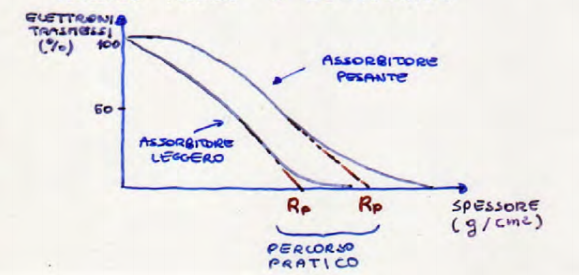
\includegraphics[scale=1]{./Immagini/RangeElettroni.png}
\caption{Percorso pratico degli elettroni}
\end{center}
\end{figure}
Inoltre \`e utilizzato il parametro $\eta$:
\begin{equation*}
\eta = \frac{\# \text{elettroni retrodiffusi}}{\# \text{elettroni incidenti}}
\end{equation*}
Per via della piccola massa degli elettroni, le interazioni con i nuclei sono fondamentali: possiamo osservare scattering multipli e perdite per irraggiamento.\\
Quest'ultimo diventa predominante a energie relativistiche, in particolare le dipendenze \textit{non relativistiche} sono:
\begin{gather*}
S_{coll} \propto \frac{1}{E_k} \, \frac{Z}{A}\\
S_{irr} \propto \frac{Z^2}{A}
\end{gather*}
mentre ad energie relativistiche diventano:
\begin{gather*}
S_{coll} \propto \frac{Z}{A}\\
S_{irr} \propto \frac{Z^2}{A}\, E_k
\end{gather*}
Si definisce \textbf{energia critica}, il valore dell'energia cinetica per cui le due $S$ si equivalgono, esso vale circa:
\begin{equation*}
E_c = \frac{550}{Z} \text{MeV}
\end{equation*}
da cui si deduce che nei materiali pesanti l'irraggiamento diventa prevalente ad energie pi\`u basse.\\
Un parametro fondamentale \`e la \textbf{lunghezza di radiazione}:
\begin{equation*}
X_0 \approx 170 \frac{A}{Z^2} \frac{\text{g}}{\text{cm}^2}
\end{equation*}
Essa indica la distanza media che un elettrone deve percorrere per osservare l'emissione di un quanto di energia comparabile a quella iniziale:\\
Per quando riguarda lo spettro, in energia esso \`e quasi costante:
\begin{equation*}
E_{\gamma} * \frac{dN_{\gamma}}{dE_{\gamma}} = \text{costante}
\end{equation*}
da cui si deduce che un elettrone emette pi\`u fotoni a minore energia rispetto a quelli a maggiore energia.\\
La distibuzione angolare dei fotoni emessi \`e perpendicolare alla direzione di moto nel caso di elettroni a bassa energia,
mentre nel caso di alta energia l'angolo di emissione tende a diventare 0.

\section{Interazione fotoni-materia}
I fotoni possono interagire con la materia essenzialmente in 3 modi:
\begin{itemize}
\item Effetto fotoelettrico
\item Effetto Compton
\item Produzione di coppie
\end{itemize}
Altri processi importanti (ma che assorbono pochissima energia) sono lo scattering Thomson (ovvero la diffusione di un onda piana da parte di un elettrone) e
lo scattering Rayleigh (diffusione elastica della luce).
Il primo effetto \`e prevalente a basse energie (ma sopra la soglia dell'energia di legame) ed ha una sezione d'urto maggiore per gli elettroni maggiormente legati.
Questo processo \`e spesso seguito da emissioni a cascata o transizioni Auger, queste ultime sono pi\`u frequenti nel caso di shell profonde di atomi pesanti.
La sezione d'urto del fotoelettrico \`e proporzionale a $Z^5$.\\
Il secondo \`e prevalente nelle energie intermedie (ovvero superiori al fotoelettrico, ma minori della produzione di coppie), a differenza degli altri due, che richiedono un atomo per assorbire il rinculo,
pu\`o avvenire su elettroni liberi. 
L'energia rilasciata aumenta all'aumentare dell'angolo di scattering e va come $(1-\text{cos} \theta)$.
La sezione d'urto di questo processo a basse energie va come quella Thomson (che \`e costante), ad alte energie dipende da $\frac{\text{log}\, E}{E}$,
per cui tende a 0. La dipendenza da Z \`e lineare, in quanto ogni elettrone reagisce indipendentemente dall'altro.\\
\section{Interazione neutroni-materia}
I neutroni interagiscono principalmente mediante l'interazione forte con i nuclei, questo significa che il loro raggio di interazione \`e nell'ordine del fm.
Hanno 3 modi di interazione principali:
\begin{itemize}
\item Diffusione elastica e anelastica, in questo caso il neutrone interagisce con il nucleo cedendo parte della propria energia.
Nel secondo caso il nucleo entra in uno stato eccitato.
\item Cattura radiativa e non radiativa, in questo caso il neutrone viene inglobato nel nucleo;
dopo l'assorbimento il nucleo pu\`o trovarsi in uno stato eccitato, in questo caso osserviamo l'emissione di radiazione: nel caso di fotoni si parla di cattura radiativa, 
mentre nel caso di emissione di $\alpha$ e protoni si parla di cattura non radiativa.
\item Fissione dei nuclei, in questo caso dopo la cattura il nucleo si trova in uno stato instabile e si scinde emettendo diversi neutroni e radiazione $\gamma$.
\end{itemize}
\begin{figure}[htbp]
\begin{center}
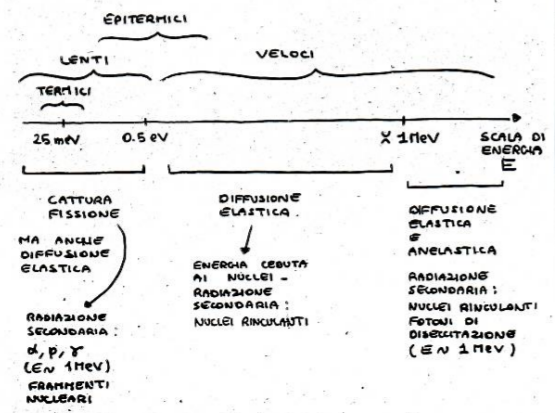
\includegraphics[scale=0.8]{./Immagini/InterazioneNeutroni.png}
\caption{Interazioni dei neutroni}
\end{center}
\end{figure}
Posta $\sigma_D$, $\sigma_C$, $\sigma_F$ la sezione d'urto dei due processi, allora la sezione d'urto totale risulta:
\begin{equation*}
\Sigma = N \, (\sigma_D + \sigma_C + \sigma_F)
\end{equation*}
con $N$ numero di nuclei per unit\`a di volume, per cui un fascio di $n_0$ neutroni seguir\`a la seguente legge:
\begin{equation*}
n(x) = n_0 \, e^{-\Sigma \, x}
\end{equation*}
Infine si definisce il libero cammino medio:
\begin{equation*}
\lambda = \Sigma^{-1}
\end{equation*}
per i neutroni veloci nell'ordine della decina di centimetri, per i lenti \`e nel centimetro.
\chapter{Cenni di statistica}
La statistica \`e fondamentale per verificare il buon funzionamento della strumentazione ed interpretare il significato delle misure sperimentali.
Si ricorda il concetto di media sperimentale e vera (coincidono solo per N elevati) e di residuo e scarto (il residuo \`e lo scarto dei dati sperimentali
dalla media sperimentale).
Inoltra si ricorda la varianza sperimentale:
\begin{equation*}
s^2 = \frac{1}{N} \sum_{i=1}^N (x_i - \bar{x})^2 = \frac{1}{N-1} \sum_{i=1}^N (x_i - \bar{x}_e)^2
\end{equation*}
dove, non conoscendo la media vera, si usa la sperimentale e si sovrastima.
\section{Distribuzioni}
Spesso si costruiscono modelli statistici per i vari processi e li si confonta con i dati sperimentali.
Modelli ricorrenti sono quello di Bernoulli:
\begin{equation*}
P(x) = \frac{n!}{(n-x)!n!} p^x (1-p)^{(n-x)}
\end{equation*}
con $n$ numero di prove, $x$ numero di prove riuscite e $p$ probabilit\`a di un successo.\\
Un altro modello \`e quello di Poisson, un approssimazione di Bernoulli per basse probabilit\`a:
\begin{equation*}
P(x) = \frac{(np)^{x} e^{-np}}{x!}
\end{equation*}
Questa distribuzione non \`e simmetrica, in quanto il valore pi\`u probabile non coincide con il valore medio $np$.\\
Un ultimo modello \`e quello di Gauss, per basse probabilit\`a e alte medie:
\begin{equation*}
P(x) = \frac{1}{\sqrt{2\pi \bar{x}}}\,\text{exp}\left(-\frac{(x-\bar{x})^2}{2\bar{x}}\right)
\end{equation*}
\section{Confronto con i dati sperimentali}
Misurata sperimentalmente $F(x)$, ovvero la distribuzione sperimentale, si pongono $\bar{x}$ e $\sigma$ nel modo definito prima e si confronta
la distribuzione con $P(x)$. 
Un primo approccio \`e grafico, per conoscere qualitativamente l'andamento, successivamente si procede con il test $\chi^2$.
\begin{equation*}
\chi^2 = \sum \frac{(x-\bar{x})^2}{\bar{x}} = (N-1)\frac{s^2}{\bar{x}}
\end{equation*}
per cui:
\begin{equation*}
\frac{\chi^2}{(N-1)} = \frac{s^2}{\bar{x}}
\end{equation*}
detto anche chi-quadro ridotto.
Se la distribuzione \`e poissoniana, esso deve essere circa 1 in quanto la varianza corrisponde alla media, o comunque tra 0.5 e 1.5; un $\chi^2$ troppo alto vuol dire che la serie di dati non \`e compatibile in quanto le
fluttuazioni sperimentali sono troppo elevate rispetto al modello, nel caso sia piccolo vuol dire che si hanno fluttuazioni troppo piccole.
\section{Singola misura}
Supponendo di poter prendere la una singola misura statistica (ad esempio un conteggio), quello che si pu\`o dire \`e che la gaussiana della distribuzione \`e centrata
su quella misura con varianza pari al valore della misura stessa. 
Ci\`o ci permetter\`a di dire che al 68\% il valore medio sar\`a tra $x-\sqrt{x}$ e $x+\sqrt{x}$.
Inoltre l'errore \% sar\`a:
\begin{equation*}
\sigma_{\%} = \frac{\sigma}{x} = \frac{1}{\sqrt{x}}
\end{equation*}
per cui l'errore diminuisce all'aumentare della statistica.
\section{Ottimizzazione dei conteggi}
Supponiamo di voler eseguire un operazione di misura di rate: abbiamo un rate $S$ dovuto alla sorgente ed un rate $B$ dovuto al fondo.
Noi siamo in grado di misurare il rate del fondo e il rate sorgente+fondo, supponendo di avere un tempo $T$ da suddividere in tempo per la
misura del fondo $T_B$ e tempo per la misura del fondo+sorgente $T_{S+B}$, come devo suddividere il mio tempo per ottenere una misura
pi\`u precisa possibile di $S$?\\
Inanzitutto:
\begin{equation*}
B = \frac{N_B}{T_B}
\end{equation*}
mentre:
\begin{equation*}
S+B = \frac{N_{S+B}}{T_{S+B}}
\end{equation*}
di conseguenza:
\begin{equation*}
S = \frac{N_{S+B}}{T_{S+B}} - \frac{N_B}{T_B}
\end{equation*}
e:
\begin{equation*}
\sigma^2_S = \left(\frac{\sigma_{N_{S+B}}}{T_{S+B}}\right)^2 + \left(\frac{\sigma_{N_B}}{T_B}\right)^2= \frac{N_{S+B}}{T^2_{S+B}} + \frac{N_B}{T_B^2}
= \frac{S+B}{T_{S+B}} + \frac{B}{T_B}
\end{equation*}
A questo punto differenziando la relazione si ha:
\begin{equation*}
2 \sigma_S d\sigma_S = - \frac{S+B}{T^2_{S+B}} dT_{S+B} - \frac{B}{T_B^2} dT_B
\end{equation*}
ponendo $d\sigma = 0$ e tenendo conto che $dT_{S+B} + dT_B=0$ quindi $\frac{dT_{S+B}{dT_{B}}} = -1$ si arriva a dire:
\begin{equation*}
\frac{T_{S+B}}{T_B}  = \sqrt{\frac{S+B}{B}}
\end{equation*}
In particolare si nota che per fondi molto intensi si ha $T_{S+B}=T_B$.
Suddividendo i tempi come trovato, ponendo $\epsilon_{\%}$ l'errore relativo su S si ha che per S intensi rispetto al fondo:
\begin{equation*}
\epsilon_{\%} = \frac{1}{ST}
\end{equation*}
per cui \`e importante avere $S$ elevati, magari migliorando l'efficienza.
Per S deboli e fondi intensi:
\begin{equation*}
\epsilon_{\%} = \frac{4B}{S^2 T}
\end{equation*}
in questo caso \`e importante ridurre il fondo, magari ottimizzando la configurazione di misura.
\section{Limiti di rivelabilit\`a}
Supponiamo di voler rivelare la presenza di una contaminazione dovuta ad un campione in un luogo.
Prima effettueremo una misura di solo fondo, poi una misura in presenza del campione, vogliamo determinare dei livelli che indichino la presenza
di un contaminante riducendo il rischio di falsi negativi e falsi positivi per fluttuazioni statistiche.
Poniamo $N_B$ la misura di tasso effettuata con solo fondo, $N_T$ la misura di tasso effettuata con il campione (quindi fondo+sorgente) e
poniamo $N_S$ il tasso dovuto unicamente alla sorgente.\\
Analizziamo il caso in cui non sia presente contaminazione: chiaramente $N_S = N_T - N_B$ con $\sigma_{S} = \sqrt{\sigma_{T}^2 + \sigma_{B}^2} = \sqrt{N_{T} + N_{B}}$.
Se non \`e presente contaminazione $\bar{N}_B = \bar{N}_T$  e $\sigma_{S}=\sqrt{2} \sqrt{N_B}$; se $N_S<0$ chiaramente non \`e presente
contaminazione, mentre se $N_S>0$ \`e necessario porre un livello di confidenza per determinare la probabilit\`a di avere un falso positivo per fluttuazioni statistiche.
In particolare se si prende un C.L. al 90\%, il 5\% dei casi sar\`a con $N_S$ negativo e il 5\% con $N_S$ positivo, per cui la probabilit\`a
di falsi negativi sar\`a del 5\%.
A un C.L. del 90\% corrisponde $1.645\sigma_S = 2.326\sigma_B$ per discriminare l'assenza di un contaminante, con un limite sui falsi positivi del 5\%.\\
Con $N_S>2.326\sigma_B$ non si pu\`o affermare che sia presente un contaminante:
per esempio se $\bar{N}_S=2.326\sigma_B$ il 50\% dei casi darebbe un falso negativo, per questo vogliamo stabilire una soglia per ridurre al di sotto del 5\% la probabilit\`a di falso negativo.
In presenza di sole fluttuazioni statistiche e $N_S<<N_B$, poniamo $N_D$ il valore minimo di $N_S$ per poter determinare la presenza di un contaminante:
$\sigma_D = \sqrt{2 N_B+N_D} \approx \sqrt{2 N_B}$, in questo caso $N_D$ potr\`a essere minore del C.L. (dando esito negativo) oppure maggiore.
Se si pone $N_D = L_C + 1.645\sigma_D \approx 4.653 \sqrt{N_B}$ avr\`o il 5\% di probabilit\`a di avere falsi negativi, in quanto
il 5\% delle fluttuazioni si pone al di sotto di $L_C$. 
Un calcolo meno approssimato porta a dire:
\begin{equation*}
N_D = 4.653 \sqrt{N_B} + 2.706
\end{equation*}
A questo punto \`e possibile definire un'attivit\`a minima della sorgente per essere individuata:
\begin{equation*}
\alpha = \frac{N_D } {\epsilon_{abs} f T}
\end{equation*}
con $\epsilon_{abs}$ efficienza assoluta del rivelatore, $f$ quantit\`a di radiazione prodotta per disintegrazione e $T$ tempo di misura.
\section{Distribuzione degli intervalli di tempo}
La poissoniana determina le probabilit\`a nei processi con rate:
\begin{equation*}
P(n) = \frac{(rt)^n e^{-rt}}{n!}
\end{equation*}
la distribuzione dei tempi tra 2 eventi successivi si calcola come la probabilit\`a di avere 0 eventi fino a $t$ ed averne uno tra $t$ e $t+dt$:
\begin{equation*}
P(0) rdt= re^{-rt}dt
\end{equation*}
La probabilit\`a che un intervallo $t$ contenga $N$ eventi si calcola come:
\begin{equation*}
P(N-1)rdt=\frac{(rt)^{N-1}e^{-rt}}{(N-1)!}rdt
\end{equation*}
\chapter{Trattamento dei segnali elettrici}
\section{Impedenze}
Tipicamente uno strumento possiede un alta impedenza di ingresso, per non perturbare il segnale e una bassa impedenza in uscita,
per minimizzare la perdita di segnale.\\
L'unica eccezione \`e data dai segnali veloci, dove problemi legati alla riflessione del segnale richiedono l'uso di impedenze adattate,
in questo caso si avr\`a attenuazione del segnale per non avere deformazioni nell'impulso.
\section{Effetto pelle}
L'effetto pelle \`e l'effetto per cui una corrente elettrica alternata tende a scorrere maggiormente lungo la superficie di un conduttore rispetto
alle regioni interne.
Il motivo di questo effetto \`e legato ai campi magnetici interni variabili (per via della corrente alternata) e quindi a correnti
indotte che impediscono il fluire della corrente all'interno del cavo.\\
Il risultato di questo fenomeno \`e un aumento della resistenza del conduttore al crescere della frequenza del segnale elettrico,
in quanto una parte del conduttore non viene utilizzata.
\section{I cavi coassiali}
Sono cavi schermati da una maglia di rame, essa funge da schermo per le interferenze a bassa e altissima frequenza (sopra i 100 kHz).
Non \`e un ottimo schermo per le frequenze intermedie (\textbf{approfondire}): in questo caso si usano cavi a doppia schermatura,
oppure si fanno passare i cavi dentro un tubo di materiale conduttore.\\
La velocit\`a di trasmissione del segnale nel cavo tipica \`e circa il 66\% di $c$, tuttavia esistono speciali cavi ritardanti dove
la velocit\`a pu\`o arrivare al 1\%; la velocit\`a \`e proporzionale a $Z = \sqrt{\frac{L}{C}}$.\\
In un cavo le \textbf{caratteristiche fondamentali} sono l'impedenza, l'induttanza e la capacit\`a per unit\`a di lunghezza.
Se il cavo deve trasportare l'alta tensione, allora \`e importante la massima tensione trasportabile.\\
\subsection{Disturbi nei coassiali}
Ogni cavo \`e soggetto a perdite dissipative legate alla resistenza del conduttore, esse sono trascurabili per lunghezze fino a qualche
decina di metri, salvo per impulsi con tempi di salita molto brevi.
Ad esempio un segnale con fronte di salita di 1 ns subisce evidenti distorsioni anche solo con cavi lunghi 3 m, per via di effetti di
riflessione dell'impulso.\\
La schermatura viene anche utilizzata serve per fare da riferimento di massa comune tra i vari dispositivi e viene connesso allo
chassis del dispositivo, ovvero l'involucro metallico dell'apparecchio.\\
Un effetto che \`e importante evitare \`e il \textbf{ground loop} (\textbf{approfondire}):
se il riferimento di massa fa una forma chiusa, per garantire un potenziale comune pu\`o circolare una corrente continua.
Questa corrente pu\`o subire fluttuazioni che generano correnti spurie nel mio segnale, disturbandolo.
Per evitare questo effetto, \`e importante che ogni strumento abbia un riferimento interno di massa, che l'alimentazione venga fornita
a stella da un unico distributore, che la massa degli strumenti coincida con quella dell'alimentatore e che la corrente venga prelevata
da una sola presa con un circuito dedicato.\\
Segnali di transiente di accensione/spegnimento di un dispositivo possono indurre correnti nella schermatura del coassiale,
provocando disturbi. 
Ad esempio i monitor dei computer introducono importanti disturbi ad alta frequenza.\\
\subsection{Metodi di abbattimento del rumore}
Per abbattere il rumore si pu\`o utilizzare un amplificatore operazionale in configurazione differenziale:
il cavo che trasporta il segnale viene intrecciato con un cavo non connesso al dispositivo, il secondo cavo serve per sondare i disturbi
ambientali a cui \`e soggetto il primo, in questo modo il preamplificatore pu\`o eliminare i disturbi comuni e pulire il segnale in gran parte (\textbf{approfondire}).
\subsection{Impedenza caratteristica e riflessione del segnale}
Nella trasmissione di segnali ci si riferisce a due casi limite:
\begin{itemize}
\item Segnali lenti o a bassa frequenza
\item Segnali veloci o ad alta frequenza
\end{itemize}
Tipicamente in un coassiale la velocit\`a di trasmissione di un segnale e 5 ns/m, se il \textit{risetime} del segnale \`e maggiore del tempo
di salita si parla di segnali \textbf{lenti}, altrimenti parliamo di segnali veloci (ad esempio succede nei segnali provenienti dagli scintillatori plastici.
\textbf{Su cavi lunghi centinaia di metri i segnali provenienti da rivelatori sono veloci.}
\subsubsection{Segnali lenti o a bassa frequenza}
Per i segnali lenti la resistenza serie del cavo \`e trascurabile, purch\'e la lunghezza del cavo non superi le centinaia di metri.\\
La capacit\`a verso massa \`e 50-100 pf/m, questa capacit\`a deve essere la pi\`u piccola possibile, in quanto si somma a quella del rivelatore;
l'ampiezza del segnale misurato \`e inversamente proporzionale a C, per quest\`o \`e importante avere cavi corti.
\subsubsection{Segnali veloci o ad alta frequenza}
\`E fondamentale considerare l'\textbf{impedenza caratteristica}: essa \`e dipendente dal dielettrico e dal diametro del conduttore centrale
e dello schermo, mentre non \`e dipendente dalla lunghezza (essa dipende dal rapporto tra induttanza e capacit\`a per unit\`a di lunghezza del cavo).
L'impedenza caratteristica \`e pari all'impedenza con la quale bisogna chiudere il cavo per poter trasmettere impulsi di tensione senza
avere effetti di riflessione del segnale.\\
Tipicamente se si chiude il cavo con un impedenza infinita si osserva riflessione totale di segnale senza sfasamenti,
mentre se si chiude il cavo con un impedenza nulla si osserva una riflessione totale, ma di verso opposto.
Quando si attacca la strumentazione il cavo vede come resistenza di terminazione la resistenza di ingresso dello strumento.
Tenendo conto che gli strumenti hanno, in generale, una resistenza di ingresso alta si deduce che in presenza di segnali veloci si osservano effetti
di riflessione (l'impedenza tipica di un cavo coassiale \`e 50 $\Omega$.
Per questo motivo quando si lavora in queste condizioni si termina il cavo con una resistenza di shunt di valore pari alla resistenza caratteristica.
Il cavo vede questa resistenza in parallelo con quella di ingresso del dispositivo: essendo quest'ultima molto maggiore dell'impedenza caratteristica
la resistenza vista diventa pari alla resistenza di shunt.\\
\`E importante tenere conto del fatto che spesso i dispositivi studiati per lavorare appositamente con segnali veloci hanno gi\`a una resistenza di ingresso di 50 $\Omega$,
per cui \`e importante verificare questo fatto.
\section{Attenuatori di segnali}
Talvolta i segnali elettrici sono troppo intensi, per questo diventa necessario ricorrere a degli attenuatori di segnale.\\
L'attenuatore pi\`u semplice che si possa pensare \`e un \textbf{partitore di tensione}, tuttavia questa tecnica porta ad avere problemi
di disturbi con segnali ad alta frequenza.\\
Un altro attenuatore utilizzato \`e l'attenuatore a T (figura~\ref{fig:attenuatoreT}), in questo attenuatore la resistenza di uscita $R_0$
pu\`o essere accoppiata con l'impedenza del cavo e ponendo $\alpha=V_i/V_o$  con le resistenze:
\begin{equation*}
R_1 = R_o \frac{\alpha - 1}{\alpha + 1}
\end{equation*}
e
\begin{equation*}
R_2 = R_o \frac{2 \alpha}{\alpha^2 - 1}
\end{equation*}
si ha l'attenuazione desiderata.
\begin{figure}[htbp]
\begin{center}
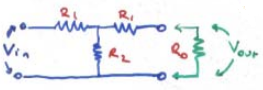
\includegraphics[scale=1]{./Immagini/AttenutatoreT.png}
\caption{Un attenuatore a T}
\label{fig:attenuatoreT}
\end{center}
\end{figure}
\section{Sdoppiamento del segnale}
Per sdoppiare i segnali lenti \`e possibile usare una T semplice, per i segnali ad alta frequenza \`e necessario prendere qualche accorgimento
aggiuntivo, la figura~\ref{fig:sdoppiatore} mostra come deve essere realizzato lo sdoppiamento:
le resistenze R sono da 16.6 $\Omega$ e vengono poste una per ogni ramo dello sdoppiamento.
Inoltre viene posto uno shunt da 16.6 $\Omega$ in parallelo allo strumento di lettura, 
in questo modo il segnale vede lungo la linea una resistenza da 50 $\Omega$ e non si subiscono riflessioni e disturbi.
Chiaramente il segnale in questo modo viene diviso in due segnali di ampiezza dimezzata rispetto all'originale.
\begin{figure}[htbp]
\begin{center}
	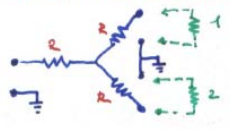
\includegraphics{./Immagini/Sdoppiatore.png}
\caption{Uno sdoppiatore di segnale ad alta frequenza}
\label{fig:sdoppiatore}
\end{center}
\end{figure}
\section{Trasformatore invertente}
Il trasformatore invertente, serve ad invertire la polarit\`a di segnali pi\`u brevi di 100 ns, in alternativa \`e necessario usare altri dispositivi ad-hoc, come gli amplificatori.
\begin{figure}[htbp]
\begin{center}
	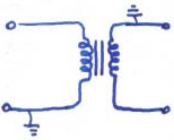
\includegraphics[scale=1.00]{./Immagini/TrasformatoreInvertente.png}
\caption{Un trasformatore invertente, il ramo dove \`e presente la messa a terra \`e invertito.}
\end{center}
\end{figure}
\section{La formatura del segnale}
Spesso \`e necessario formare un segnale, ovvero fare in moto che abbia determinati tempi di salita e di discesa dell'impulso,
questo pu\`o essere ottenuto con dispositivi passivi o attivi.
\subsection{Differenziatore CR o filtro passa-alto}
\begin{figure}[htbp]
\begin{center}
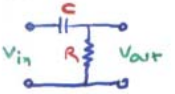
\includegraphics[scale=1]{./Immagini/FiltroCR.png}
\caption{Filtro passa-alto}
\label{fig:filtroCR}
\end{center}
\end{figure}
Il filtro passa-alto (fig.~\ref{fig:filtroCR}) pu\`o essere utilizzato per formare il fronte di discesa di un segnale:
all'aumentare della frequenza di taglio ($\propto \tau^{-1}=(RC)^{-1}$) la componente in bassa frequenza del segnale viene smorzata, lasciando solamente le alte frequenze che vanno a 0 pi\`u velocemente.
In conclusione al diminuire di $\tau$ il segnale aumenta la propria velocit\`a di smorzamento.
Questo filtro elimina la componente in bassa frequenza ($\omega \cdot \tau \ll 1$) del segnale, lasciando i segnali sinusoidali ad alta frequenza ($\omega \cdot \tau \gg 1$) inalterati.\\
Un segnale in uscita dal preamplificatore pu\`o essere approssimato con un gradino
\begin{equation*}
V_in(t) = \begin{cases}
0 \text{ se }t<0\\
V_0 \text{ se }t\ge 0
\end{cases}
\end{equation*}
in quanto possiede un fronte di salita molto veloce ed un fronte di discesa molto lento (quasi piatto).
Un segnale di questa forma che entra in un CR esce con questa formatura
\begin{equation*}
V_{out}(t) = V_0 e^{-t/\tau} 
\end{equation*}
ovvero con un fronte di discesa formato. 
Questo perch\`e il fronte di salita essendo veloce (quindi formato quasi unicamente da componenti ad alta frequenza) passa inalterato, mentre il fronte di discesa,
essendo lento (quindi formato quasi unicamente da armoniche a bassa frequenza), viene determinato da quali frequenze basse vengono fatte passare.
\subsection{Integratore RC o filtro passa-basso}
\begin{figure}[htbp]
\begin{center}
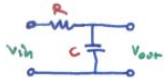
\includegraphics[scale=1]{./Immagini/FiltroRC.png}
\caption{Filtro passa-basso}
\label{fig:filtroRC}
\end{center}
\end{figure}
Il filtro passa-basso (fig.~\ref{fig:filtroRC}) pu\`o essere utilizzato per formare il fronte di salita di un segnale:
all'aumentare della frequenza di taglio ($\propto \tau^{-1}=(RC)^{-1}$) vengono ammesse nuove componenti ad alta frequenza che, avendo derivata maggiore, fanno salire il segnale pi\`u rapidamente.
In conclusione al diminuire di $\tau$ il segnale aumenta la propria velocit\`a di smorzamento.
Questo filtro elimina la componente in bassa frequenza ($\omega \cdot \tau \ll 1$) del segnale, lasciando i segnali sinusoidali ad alta frequenza ($\omega \cdot \tau \gg 1$) inalterati.\\
Un segnale in uscita dal preamplificatore pu\`o essere approssimato con un gradino
\begin{equation*}
V_in(t) = \begin{cases}
0 \text{ se }t<0\\
V_0 \text{ se }t\ge 0
\end{cases}
\end{equation*}
Un segnale di questa forma che entra in un RC esce con questa formatura
\begin{equation*}
V_{out}(t) = V_0 (1-e^{-t/\tau})
\end{equation*}
ovvero con un fronte di salita formato. 
Questo perch\`e il fronte di salita essendo veloce (quindi formato quasi unicamente da componenti ad alta frequenza) viene determinato da quali frequenze vengono ammesse,
mentre il fronte di discesa, essendo lento (quindi formato quasi unicamente da armoniche a bassa frequenza), passa inalterato.
\subsection{Formatura CR-RC}
Se io combino i due filtri precedentemente descritti frapponendo fra i due un amplificatore operazionale (fig~\ref{fig:filtroCRRC}) di disaccoppiamento con guadagno pari a 1,
si ottiene una catena di lettura in grado di formare sia il fronte di salita che il fronte di discesa dell'impulso.
\begin{figure}[htbp]
\begin{center}
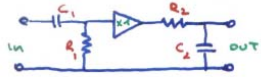
\includegraphics[scale=1]{./Immagini/FiltroCRRC.png}
\caption{Formatura tramite un CR-RC}
\label{fig:filtroCRRC}
\end{center}
\end{figure}
Se supponiamo di sottoporre la catena ad un gradino di tensione di ampiezza $V_0$ (approssima bene i segnali in uscita da un preamplificatore), in uscita si otterr\`a:
\begin{equation*}
V(t) = V_0 \, e^{-t/\tau_2}(1 - e^{-t/\tau_1}) 
\end{equation*}
Se $\tau_1 \approx \tau_2$ e sviluppando al primo ordine il termine tra parentesi si ottiene:
\begin{equation*}
V(t) = V_0 \, e^{-t / \tau} \frac{t}{\tau}
\end{equation*}
Il tempo caratteristico del RC (passa basso) determina il fronte di salita: diminuendo $\tau$ (=$RC$) aumenta la frequenza di taglio, per cui si allarga la banda di basse frequenze ammesse, aumentando la velocit\`a di salita.
Il tempo caratteristico del CR (passa alto) determina il fronte di discesa: se $\tau$ aumenta, la frequenza di taglio diminuisce, introducendo componenti a bassa frequenza che rallentano la discesa del segnale.
In conclusione aumentare $\tau_{RC}$ aumenta la velocit\`a di salita, aumentare $\tau_{CR}$ diminuisce la velocit\`a di discesa.\\
Le costanti di tempo devono essere scelte in modo tale da poter raccogliere le cariche disponibili, ridurre il rumore elettronico ed evitare il \textit{pile-up}.
In particolare alcune richieste sono in contrapposizione, ad esempio per essere sicuri di raccogliere tutte le cariche pu\`o essere utile avere un tempo di discesa lungo, 
tuttavia questo aumenta il rischio di avere del \textit{pile-up}. 
\begin{figure}[htbp]
\begin{center}
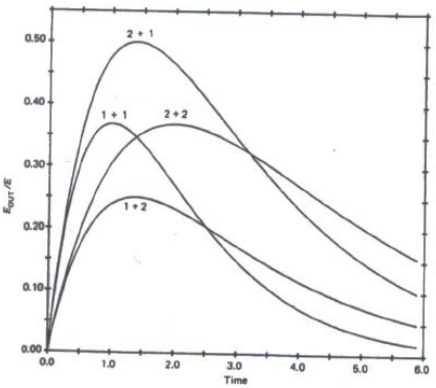
\includegraphics[scale=1]{./Immagini/FormaturaRCCR.png}
\caption{Esempi di segnali formati con varie costanti di tempo}
\label{fig:formaturaRCCR}
\end{center}
\end{figure}
\subsection{Formatura gaussiana}
Costruendo un circuito CR-(RC)$^n$ con n RC in cascata si pu\`o ottenere una formatura gaussiana dell'impulso:
\begin{equation}
V(t) = V_0 \, e^{-t/\tau} (1-e^{-t/\tau})^n \approx V_0 \left(\frac{t}{\tau}\right)^n e^{-t/\tau}
\end{equation}
Questa forma per $n>4$ approssima bene una gaussiana;
il massimo viene raggiunto in $n\tau$, detto anche \textit{\textbf{peaking time}}).
A parit\`a di \textit{peaking time}, questa formatura recupera la linea di base pi\`u velocemente rispetto alla formatura RC-CR.
Questa formatura \`e la migliore in qualit\`a di rapporto segnale-rumore.
\subsection{Formature con fitri attivi}
Utilizzando circuiti con elementi attivi come diodi o transistor si possono ottenere formature pi\`u fantasiose.
\begin{itemize}
\item \textbf{Formatura triangolare}, ottenibile con una serie di filtri attivi
\item \textbf{Formatura trapezoidale}, utilizzata se il risetime \`e variabile, in modo da avere tutta la carica raccolta in rivelatori con grande variabilit\`a di tempi di risposta.
Questa formatura viene ottenuta con circuiti analogici e digitali.
\end{itemize}
\subsection{Formatura CR-RC-CR}
Utilizzata per dare una forma bipolare all'impulso nel caso di rate molto elevati.
\subsection{Formatura con singola linea di ritardo}
La singola linea di ritardo (SDL) viene utilizzata per ridurre la durata di impulsi troppo lunghi:
un segnale viene sdoppiato in due rami, uno \`e il ramo di output, l'altro viene lasciato aperto.
Se il tempo di propagazione $\tau$ in quest'ultimo \`e molto maggiore del tempo di salita dell'impulso, allora dopo $2 \tau$ il segnale ritorna identico sulla linea di output, 
ma invertito.
Sommandosi al segnale precedente lo annulla.
\begin{figure}[htbp]
\begin{center}
	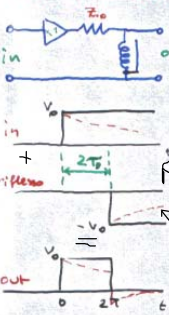
\includegraphics[scale=1]{./Immagini/SDL.png}
	\caption{Formatura con SDL (Single Delay Line)}
\label{fig:SDL}
\end{center}
\end{figure}
Nel caso il segnale avesse un tempo decadimento si pu\`o presentare il problema dell'\textit{undershoot} (tratteggio rosso nell'immagine): per risolverlo
\`e necessario attenuare in modo opportuno il segnale lungo la linea di ritardo.
\subsection{Formatura con doppia linea di ritardo}
\`E possibile rendere il segnale bipolare imponendo un'altra linea di ritardo in uscita dalla SDL con lo stesso tempo della prima linea.
Il problema di questa formatura \`e che non passa da filtri, per cui presenta il problema del rumore non filtrato, per questo viene usata prevalentemente
in rivelatori con poca risoluzione o per i segnali logici.
\section{Cancellazione del polo zero}
Nella realt\`a i nostri dispositivi non sono sottoposti a dei gradini, bensi a segnali che salgono molto velocemente e decadono molto lentamente.
I tempi di decadimento possono portare a degli \textit{undershoot} che vengono recuperati in tempi nell'ordine dei $\mu$s causando problemi nella forma degli
impulsi successivi. \\
Si dimostra che nei CR-RC il problema pu\`o essere risolto utilizzando una resistenza regolabile in parallelo alla capacit\`a nel CR.
\section{Spostamenti della linea di base}
Supponiamo di avere un treno di impulsi, poich\`e in un CR-RC la tensione media deve essere nulla, in caso di alti rate si pu\`o osservare uno spostamento
della linea di base in modo da mantenere tale media nulla.\\
Nel caso di impulsi identici equispaziati lo spostamento non \`e problematico in quanto costante, tuttavia nella realt\`a gli impulsi hanno forma diversa per cui lo spostamento
pu\`o risultare un problema.\\
Per risolvere il problema si pu\`o usare una formatura bipolare in modo da compensare questo effetto, tuttavia porta ad avere alti rapporti rumore-segnale.
Un'altra soluzione proviene dall'accoppiare il segnale in tensione continua che successivamente viene eliminato con un filtro.
\chapter{Impulsi lineari e impulsi logici}
Un \textbf{impulso lineare} \`e un impulso la cui informazione \`e contenuta nell'ampiezza e nella forma, un \textbf{impulso logico} \`e un impulso la cui informazione
\`e contenuta nel fatto che esso sia presente o meno e nell'istante in cui appare.\\
In genere una catena di acquisizione registra un impulso lineare, lo manipola e, ad un certo punto, lo trasforma in una serie di impulsi logici che vengono registrati.
\section{Classificazione degli impulsi lineari}
Gli impulsi lineari vengono classificati in:
\begin{itemize}
\item Impulsi veloci
\item Impulsi lenti
\item Impulsi dopo formatura
\end{itemize}
\subsection{Impulsi veloci}
Gli impulsi veloci sono segnali che vengono raccolti in circuiti con $\tau$ caratteristica molto piccola,
essi hanno quindi un \textit{rise time} e \textit{decay time} determinato dalle caratteristiche di raccolta della carica del rivelatore.
In genere questi impulsi hanno una \textbf{durata inferiore} a qualche $\mu$s e sono pi\`u \textbf{piccoli in ampiezza} (la polarit\`a viene determinata dall'alimentazione del rivelatore), per questo motivo soffrono di un \textbf{rapporto segnale-rumore peggiore}.\\
Gli impulsi veloci servono per trasformare informazioni temporali in quanto il fronte di salita ripido aumenta la risoluzione del dispositivo.
\subsection{Impulsi lenti}
All'opposto dei veloci, gli impulsi lenti sono segnali che vengono raccolti in circuiti con $\tau$ caratteristica grande. 
In genere il fronte di salita viene determinato dai tempi di raccolta della carica, mentre il fronte di discesa dalla $\tau$ caratteristica del circuito di raccolta,
per questo la $\tau$ viene scelta in modo da evitare il \textbf{deficit balistico}, ovvero lo smorzamento del segnale prima della raccolta completa della carica.
Per questo motivi vengono anche chiamati \textit{\textbf{tail pulses}} per via del fronte di discesa lungo.\\
Questi impulsi hanno un'ampiezza alta rispetto agli impulsi veloci e la loro polarit\`a e variabile, anche se spesso \`e negativa.
In conclusione, in questi segnali sono importanti l'ampiezza e il rise time (ovvero il tempo impiegato per passare dal 10\% al 90\% dell'ampiezza).
\subsection{Impulsi dopo formatura}
Sono impulsi lenti con tempi di decadimento nei microsecondi, in genere gli impulsi vengono formati per adattarli ai circuiti di lettura e analisi.
\section{Impulsi logici}
Esistono tre categorie:
\begin{itemize}
\item Impulsi logici standard (o TTL)
\item Impulsi logici NIM
\end{itemize}
\subsection{Impulsi TTL}
Sono impulsi a polarit\`a positiva, il livello 0 viene riconosciuto per tensioni tra -2V e 0V, mentre il livello 1 tra +4V e +12V.
La durata dell'impulso \`e nei $\mu$s e hanno una forma d'onda quadra.
\subsection{Impulsi veloci NIM}
Sono impulsi con tempi di salita nel ns (\`e necessario prendere cautele per effetti di riflessione), la loro polarit\`a \`e negativa e il segnale \`e in corrente.
L'ampiezza per il segnale 0 \`e tra -1mA e +1mA, per il segnale 0 \`e tra -14mA e -18mA.
\subsection{Impulsi di gate}
\textbf{NON sono impulsi logici}, serve a comandare e determinare il momento in cui un dispositivo \`e attivo e riceve segnale.
Ha la forma di un'onda quadra.
\section{Dispositivi per il trattamento degli impulsi}
\subsection{Linear-Linear}
\begin{itemize}
\item \textbf{Preamplificatore}, riceve in ingresso della carica e produce un impulso lineare a coda lunga 
\item \textbf{Amplificatore lineare}, riceve in ingresso un impulso lineare a coda lunga e produce un impulso formato ed amplificato
\item \textbf{Amplificatore a soglia}, riceve in ingresso un impulso formato e produce un segnale lineare proporzionale all'ampiezza del segnale in ingresso oltre la soglia.
\item \textbf{Allungatore di impulsi (\textit{Pulse stretcher}}, riceve un segnale lineare veloce in ingresso e produce un segnale formato della stessa ampiezza del segnale in input
%% elemento 5
\item \textit{Amplificatore sommatore}, riceve in ingresso pi\`u impulsi lineari formati e produce un segnale pari alla somma dei segnali in ingresso
\item \textbf{Modulo dei ritardi}, riceve un segnale e produce lo stesso segnale dopo un certo lasso di tempo
\item \textbf{Gate lineare}, riceve un impulso formato ed un impulso di gate e produce un segnale identico al segnale lineare se esso \`e in coincidenza con il gate
\end{itemize}
\subsection{Linear-Logic}
\begin{itemize}
\item \textbf{Discriminatori integrali}, riceve un impulso formato e produce un impulso logico se esso supera un livello di discriminazione
\item \textbf{Discriminatori differenziali}, riceve un impulso formato e produce un segnale logico se esso \`e compreso in una certa finestra di accettanza
\end{itemize}
\subsection{Logic-Linear}
\begin{itemize}
\item \textbf{Time to amplitude converter}, riceve in ingresso 2 segnali logici e produce un segnale lineare proporzionale all'intervallo di tempo tra l'arrivo dei due segnali
\end{itemize}
\subsection{Logic-Logic}
\begin{itemize}
\item \textbf{Modulo di coincidenza}, riceve impulsi logici e produce un segnale logico se essi appaiono entro un certo $\tau$ detto \textbf{resolving time}
\item \textbf{Modulo di anticoincidenza}, riceve impulsi logici e produce un segnale logico se si presenta un impulso solo in uno degli ingressi entro un $\tau$
\item \textbf{Scaler}, produce un impulso logico ogni tot impulsi logici
\end{itemize}

\section{Preamplificatori}
Se un dispositivo produce una quantit\`a di carica piuttosto elevata (come ad esempio un rivelatore Geiger) la tensione prodotta tramite la capacit\`a del rivelatore
pu\`o essere sufficiente per ottenere un impulso misurabile.
Spesso, tuttavia, \`e necessario utilizzare un \textbf{preamplificatore} (PRE) per aumentare l'ampiezza dell'impulso.\\
Questi dispositivi vengono messi molto vicini fisicamente ai rivelatori, per ridurre la capacit\`a dei cavi (la tensione \`e inversamente proporzionale alla capacit\`a),
hanno una resistenza di uscita molto bassa (per avere un $\tau = RC$ piccolo e non integrare il segnale), mentre quella in ingresso \`e molto elevata (per raccogliere completamente la carica).
Il segnale prodotto dal PRE \`e un segnale a coda lunga, in modo da non essere vincolante per la catena elettronica a seguire, in particolare il fronte di salita ha
tempi caratteristici molto brevi, mentre quello di discesa ha tempi nell'ordine dei 50-100 $\mu s$.\\
\subsection{Configurazioni dei preamplificatori}
\begin{figure}[htbp]
\begin{center}
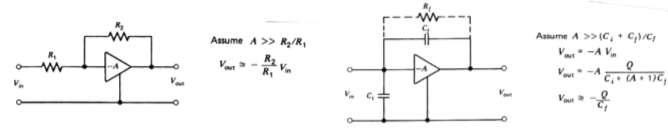
\includegraphics[scale=0.6]{./Immagini/ConfigurazioniPRE.png}
\caption{Configurazione voltage e charge sensitive}
\label{fig:configurazioniPRE}
\end{center}
\end{figure}
A sinistra nella figura~\ref{fig:configurazioniPRE} si vede la configurazione \textbf{voltage sensitive} del PRE:
se a monte del PRE \`e presente una capacit\`a costante il segnale in ingresso dal rivelatore sar\`a $Q/C$ per cui in uscita dal rivelatore,
se l'OP. AMP. ha un fattore di amplificazione sufficientemente grande, si ha un segnale pari a:
\begin{equation*}
V_{out} = - \frac{R_f}{R_i} V_{max} \propto Q
\end{equation*}
In molti rivelatori (come quelli a semiconduttore) la capacit\`a non \`e costante, per questo si opta per la configurazione \textbf{charge sensitive}:
Viene introdotta in parallelo a $R_f$ una capacit\`a di feedback, se l'amplificazione del OP. AMP. \`e sufficientemente grande allora:
\begin{equation*}
V_{out} = -A \frac{Q}{C_i + (A+1) C_f} \approx \frac{Q}{C_f}
\end{equation*}
In questo modo \`e possibile imporre una capacit\`a a piacere.
\subsection{Polarizzazione del rivelatore}
La tensione di polarizzazione del rivelatore pu\`o essere fornita attraverso la linea del preamplificatore.
Esistono due possibili configurazioni utilizzabili per fornire tale tensione, una accoppiata in AC e una accoppiata in DC.
\begin{figure}[htbp]
\begin{center}
	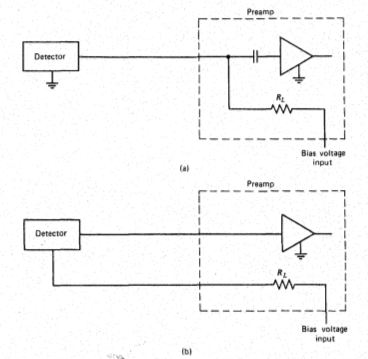
\includegraphics[scale=1]{./Immagini/TensPolarizzazione.png}
\caption{a) Accoppiamento in AC b) Accoppiamento in DC}
\label{fig:tensPolarizzazione}
\end{center}
\end{figure}
\subsubsection{Configurazione AC-coupled}
\`E la configurazione a) in figura~\ref{fig:tensPolarizzazione}, in questa configurazione la tensione di polarizzazione e la corrente di buio passano attraverso
la linea di resistenza $R_L$, il rivelatore \`e a massa.\\
Un condensatore di disaccoppiamento \`e posto all'ingresso del PRE in modo da poter scegliere $R_L$ senza modificare il segnale in uscita dal rivelatore.
La resistenza $R_L$ deve essere grande in modo da ridurre al minimo il rumore, tuttavia non pu\`o superare un certo valore in quanto attraverso di esse passa la corrente
di buio.
In presenza di correnti di buio troppo elevate si possono osservare cadute di tensione elevate lungo la linea, facendo cadere la tensione di polarizzazione applicata al rivelatore.
Per questo motivo la resistenza deve essere scelta in modo adeguato; in questi casi pu\`o essere utile regolare la tensione di polarizzazione fornita tenendo conto di questo fenomeno.
\subsubsection{Configurazione DC-coupled}
In questa configurazione la tensione di polarizzazione viene fornita direttamente al rivelatore che viene isolato dalla massa. 
Questa modalit\`a porta a rumori minori, tuttavia ha dei problemi legati al fatto che il segnale \`e accoppiato alla tensione di polarizzazione:
ci\`o implica che resistenze $R_L$ diverse possono portare a segnali diversi.
Dato che la corrente di buio passa dal PRE, in particolare dalla resistenza di feedback, correnti troppo elevate possono portare a segnali distorti per via delle tensioni
ai capi della resistenza. 
Un'alternativa \`e dato dall'uso di capacit\`a di feedback che integrano la corrente, poich\`e i segnali del PRE possono essere approssimati come dei gradini
questo significa che il fronte orizzontale diventer\`a crescente portando gradualmente alla saturazione del PRE.
I PRE possiedono sistemi di reset che, in presenza di una saturazione, riavviano il sistema, tuttavia essi introducono maggiori tempi morti.
Per questo in caso di correnti di buio molto intense possono portare a saturazioni pi\`u frequenti, per questo in tali casi l'accoppiamento in AC risulta una scelta obbligata.
\subsection{Preamplificatori nei vari rivelatori}
La catena elettronica di base in un preamplificatore \`e molto simile in tutti i rivelatori, con adattamenti a seconda delle caratteristiche del rivelatore.
Ad esempio i preamplificatori nei rivelatori a gas hanno correnti di buio minori, per questo \`e possibile introdurre resistenza $R_L$ molto elevate, per attenuare il rumore;
nei rivelatori a semiconduttore questo non pu\`o avvenire, in quanto le correnti sono maggiori.\\
Un'altra differenza pu\`o essere data dalla tensione di polarizzazione e dal suo isolamento, un rivelatore a gas richiede tensioni nell'ordine delle migliaia di volt,
mentre un semiconduttore nell'ordine delle centinaia, con la differenza che i cavi possono avere isolamenti differenti.\\
I segnali in uscita da un tubo fotomoltiplicatore di uno scintillatore sono piuttosto elevati, per questo i preamplificatori in questi rivelatori non hanno
caratteristiche troppo spinte, in quanto i problemi legati all'amplificazione ed al rumore sono ridotti. 
Per questo motivo i PRE hanno principalmente il ruolo di fissare il tempo caratteristico di un segnale.
Negli scintillatori \`e possibile lavorare anche con il segnale anodico, quindi in assenza di preamplificatore, in queste condizioni la forma del segnale
\`e fortemente dipendente dalla carattestiche fisiche dei cavi (come ad esempio la loro capacit\`a) e dell'elettronica a cascata e spesso la $\tau$ indotta da queste carattestiche pu\`o non essere ottimale.
I PRE generalmente non forniscono la tensione di alimentazione dello scintillatore, mentre l'alta tensione agisce sul tubo fotomoltiplicatore.
\subsection{Limite sul tasso di conteggi per la saturazione}
Un PRE pu\`o saturare in seguito ad un impulso eccessivo oppure in seguito a rate troppo elevati per pile-up in quanto la coda dell'impulso \`e lunga.\\
Una soluzione pu\`o venire dal diminuire il tempo caratteristico di discesa del segnale, tuttavia questo aumenta il rumore, in quanto entrano in banda passante 
nuove basse frequenze.\\
Se il rivelatore \`e accoppiato in continua allora la tensione di saturazione \`e data dalle correnti che provengono dal rivelatore, in particolare
se nel rivelatore viene depositata un energia $E$ e l'energia media di ionizzazione vale $\epsilon$, la carica liberata risulta:
\begin{equation*}
Q = \frac{E\cdot e}{\epsilon}
\end{equation*}
La corrente di saturazione sar\`a data dal rapporto tra la tensione di saturazione e la resistenza di feedback e sar\`a collegata ad un tasso massimo di ionizzazioni
che \`e possibile produrre, che indichiamo con $r_m$:
\begin{equation*}
I_{sat} = \frac{V_{sat}}{R_f} = \frac{E \cdot e}{\epsilon} \cdot r_m
\end{equation*}
Da questa relazione \`e possibile calcolare $r_m$ a partire dalle caratteristiche del PRE, in particolare \`e di interesse il limite \textbf{energia-rate}, ovvero
la quantit\`a massima di energia che si pu\`o mediamente misurare senza saturare il dispositivo:
\begin{equation*}
E \cdot r_m = \frac{V_{sat} \, \epsilon}{e\, R_f}
\end{equation*}
Per un rivelatore HPGe (High Purity GErmanium) ($\epsilon = 2.96$ eV) con $V_m = 10$ V e $R_f = 1$ G$\Omega$ esso vale $1.85 \cdot 10^5$ MeV/s.
\section{Amplificatori lineari}
L'amplificatore ha il ruolo di effettuare l'amplificazione e la formatura del segnale.
Il PRE preleva la propria alimentazione dall'amplificatore, per questo pu\`o essere soggetto a ground loop, in tal caso pu\`o essere necessario alimentare il dispositivo separatamente.
Tipicamente l'amplificatore \`e in grado di produrre in uscita segnali lineari tra i 0 e i 10 V, se il segnale in ingresso \`e maggiore di 10 V l'amplificatore satura,
distorcendo il segnale.
Il fattore di amplificazione deve essere scelto tenendo conto di questo fenomeno.\\
Per quanto riguarda la formatura del segnale, esse deve essere scelta in base ai rate di conteggio, la risoluzione, il rapporto segnale-rumore, il deficit balistico
e il pile-up.\\
In genere in caso di alti rate \`e meglio avere impulsi bipolari di larghezza limitata, per ridurre il pile-up, in caso di bassi rate queste restrizioni non sono presenti
per cui \`e meglio avere impulsi unipolari lenti, in modo da massimizzare la risoluzione energetica.\\
A bassi rate gli effetti collegati a pile-up e spostamenti della linea di base sono ininfluenti, per questo \`e meglio avere segnali con tempi caratteristici lunghi,
per minimizzare il rumore serie, tuttavia tempi caratteristici troppo lunghi possono aumentare il rumore per via del rumore parallelo, per questo esiste un valore ottimale.\\
Ad alti rate si ha un generale peggioramento del rumore, per via di problemi di pile-up e spostamento della linea di base, per questo il minimo si sposta
a tempi caratteristici inferiori, in generale per tempi caratteristici molto bassi gli effetti di alto rate vengono abbattuti e il rumore ritorna simile a
quello a basso rate.\\
Per sistemi a bassa risoluzione, in presenza di bassi rate, qualunque formatura va bene, mentre in presenza di alti rate \`e preferibile una formatura con
doppia linea di ritardo.\\
Nel caso di sistemi ad alta risoluzione per bassi rate \`e preferibile una formatura gaussiana o triangolare, mentre per alti rate una bipolare (per gli scostamenti
della linea di base).\\
\`E importante evitare che l'amplificatore saturi, specie ad alti rate, in quanto il tempo di recupero diventa maggiore in caso di saturazione, per questo \`e
importante avere un circuito che attivamente ristabilisca la linea di base.\\
In conclusione un amplificatore deve:
\begin{itemize}
\item Amplificare il segnale
\item Formare il segnale in modo da ottimizzare la misura di interesse
\item Formare il segnale in modo da evitare pile-up e saturazioni
\item Ottimizzare il rapporto segnale-rumore
\item Fornire circuiti di reiezione del pile-up e ristabilire in modo attivo la linea di base
\end{itemize}
\begin{figure}[htbp]
\begin{center}
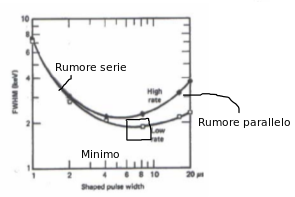
\includegraphics[scale=1]{./Immagini/RumoreSerieParallelo.png}
\caption{Rumore in funzione di rate e formatura}
\label{fig:RumoreSerieParallelo}
\end{center}
\end{figure}
\subsection{Amplificatori a soglia}
Sono dispositivi che amplificano la parte di impulsi sopra una determinata soglia, sono utili per analizzare particolari regioni dello spettro spalmandolo su tutto l'MCA.
Dato che esso registra la porzione di impulso sopra soglia, spesso questi segnali sono stretti, per questo \`e seguito da un pulse stretcher che dilata l'impulso
rendendolo analizzabile.
\section{Sistemi di conteggio}
\begin{figure}[htb]
\begin{center}
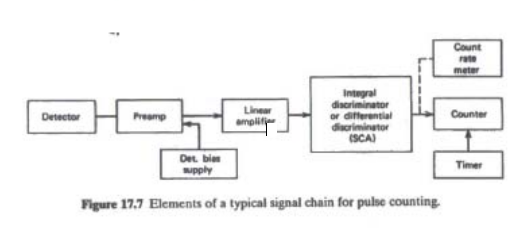
\includegraphics[scale=0.7]{./Immagini/CatenaConteggio.png}
\label{fig:catenaConteggio}
\end{center}
\end{figure}
Un sistema di conteggio deve misurare il rate di rivelazione.
\subsection{Discriminatori}
La presenza di un segnale in uscita dall'amplificatore viene verificata da un discriminatore a soglia.\\
Un discriminatore integrale produce un impulso logico se il segnale supera una determinata soglia, un discriminatore differenziale (o SCA, single channel analyzer) lo fa se il segnale entra
in una particolare finestra.
Spesso quest'ultimo \`e in grado di produrre segnali con un certo ritardo, scorrelando temporalmente il segnale.
\subsection{Contatori o scaler}
Lo scaler conta il numero di impulsi; esso pu\`o lavorare in due modalit\`a: in \textbf{preset time} il contatore conta il numero di impulsi in un determinato tempo
in base ad un clock interno o esterno, in \textbf{pulse count} esso fissa il numero di conteggi da raggiungere.\\
In questo dispositivo \`e fondamentale conoscere la risoluzione temporale o ''pulse pair resolving time`` per determinare l'intervallo di tempo
minimo tra due impulsi per essere conteggiati, in quanto essa determina il tasso massimo misurabile dal dispositivo.
\subsection{Tempo morto nei sistemi di conteggio}
\`E importante introdurre una correzione per il tempo morto del sistema, se esso \`e costante \`e possibile introdurla, mentre se esso varia, si fa in modo
di renderlo costante imponendolo come il pi\`u alto di tutta la catena.\\
Il tempo morto spesso non \`e determinato dal rivelatore (salvo contatori Geiger-Muller), ma dall'elettronica a cascata.
Il dispositivo con i tempi morti maggiori \`e il discriminatore, dove esso vale 1-2 $\mu$s pi\`u la durata dell'impulso.
\section{Analisi dell'ampiezza degli impulsi}
In generale rivelatori con FWHM media non necessitano di elettronica spinta, tuttavia per rivelatori ad alta risoluzione \`e necessario porre molta cura nella catena
di trattamento del segnale.\\
Il componente prioritario \`e dato dall'amplificatore, che, in caso di alte risoluzioni, deve utilizzare una formatura del segnale ottimale.
La strategia da usare deve essere in funzione del rate da analizzare, definiamo il \textbf{duty cicle}:
\begin{equation*}
D.C. = \Delta t \cdot r
\end{equation*}
con $r$ rate di impulsi.
Se il duty cicle \`e inferiore a $10^{-3}$ si pu\`o procedere con l'ottimizzazione della catena elettronica, se esso \`e maggiore di $10^{-1}$ \`e necessario
ridurre il rate in quanto si rischia di avere conflitti nell'elettronica.
\subsection{Deficit balistico}
Il deficit balistico consiste nel taglio dell'ampiezza del segnale per via della formatura.
In generale se la forma dell'impulso \`e costante allora la frazione tagliata \`e costante ed \`e possibile introdurre una correzione impulso per impulso,
altrimenti si assiste ad un peggioramento della risoluzione.\\
In alternativa risulta necessario allungare il tempo di salita dell'impulso, a scapito del rapporto segnale-rumore e del pile-up.
\section{Rumore}
Il rumore \`e una fluttuazione che si sovrappone al segnale in uscita dal dispositivo che degrada la FWHM, 
specialmente se esso si presenta nella regione iniziale della catena, dove il segnale \`e ancora piccolo.\\
Il rumore ha un proprio spettro che spazia dalle basse alle alte frequenze, in questo caso si parla di \textbf{rumore bianco}.
Posso distinguere il rumore bianco in \textbf{rumore serie} e \textbf{rumore parallelo}:
\begin{itemize}
\item il rumore serie \`e quello collegato a rumore termico nel FET o rumore Johnson (termico) nelle resistenze 
\item il rumore parallelo \`e legato a fluttuazioni della corrente di buio
\end{itemize}
Posso ridurre il rumore utilizzando filtri passa-alto e passa-basso che tagliano le frequenze in cui \`e presente unicamente il rumore.\\
Il rumore viene misurato in ENC (Equivalent Noise Charge): posto $v_{rms}$ la deviazione standard della distribuzione del rumore, ENC \`e il numero
di elettroni che, posto all'ingresso del PRE, produce una tensione pari a $v_{rms}$.
Dal ENC si ricava la FWHM attraverso la relazione:
\begin{equation*}
\text{FWHM} = \text{ENC} \cdot 2.35 \cdot \epsilon
\end{equation*}
\subsection{Microfonismo}
\`E un rumore dovuto a vibrazioni meccaniche nel dispositivo che modificano la capacit\`a, sono effetti piccoli che risultano visibili
solo in rivelatori con $C_{in}$ piccola. 
Il problema pu\`o essere risolto con filtri passa-basso, in quanto il rumore \`e a bassissima frequenza.
\subsection{Formatura e rumore}
Aumentando il tempo di formatura il rumore serie diminuisce, ma aumenta quello parallelo.
In aggiunta, esiste un terzo tipo di rumore, detto rumore 1/f, che non dipende dallo shaping time.
I tre rumori si combinano con una somma in quadratura:
\begin{equation*}
N^2 = N_S^2 + N_P^2+N_{1/f}^2
\end{equation*}
Esiste una formatura ottimale per cui i rumori serie e parallelo si compensano, tipicamente nei $\mu$s per i rivelatori a Si o Ge.\\
Dal punto di vista matematico, la cuspide infinita sembra avere il miglior rapporto segnale-rumore, tuttavia questa forma ha diversi problemi pratici:
ha il massimo a punta, il quale \`e difficilmente misurabile, ha una durata lunga, dando problemi di pile-up, ed \`e difficile da ottenere in pratica.
\section{L'impulso di gate}
L'impulso di gate comanda l'acquisizione del segnale, esso deve essere pi\`u lungo della durata del segnale e i dispositivi che utilizzano un gate devono attivarsi velocemente
quando esso si presenta.
\section{Tiratore di impulsi}
Produce impulsi di forma standard di ampiezza pari a quella in ingresso, viene utilizzato in presenza di impulsi veloci o stretti, per adattarli all'elettronica.
\chapter{Misure temporali}
\section{Trattamento digitale del segnale}
Esistono sistemi spettroscopici digitali, essi si occupano di amplificare e formare il segnale, correggere il polo zero, ristabilire la linea di base,
controllare la stabilit\`a del guadagno e altro.\\
Il punto fondamentale \`e dato dalla velocit\`a di campionamento dell'ADC (Analog to Digital Converter), esso, infatti, campiona e digitalizza i punti con una
certa frequenza; l'inverso di questa frequenza rappresenta la massima precisione temporale che posso raggiungere con il campionamento scelto, 
questa precisione diventa critica quando si trattano segnali veloci, inoltre il campionamento deve essere tale da preservare la forma dell'impulso.\\
Questi problemi devono essere affrontati per ottenere dei grandi vantaggi quali:
\begin{itemize}
\item Una ampia flessibilit\`a nella scelta della formatura con possibilit\`a di utilizzo di formature speciali
\item Un'ottima stabilit\`a del sistema
\item L'eliminazione del rumore dovuto all'elaborazione di segnali lineari
\item Linearit\`a del sistema
\item La possibilit\`a di introdurre ritardi senza distorcere il segnale
\end{itemize}
\section{Il convertitore analogico-digitale}
L'ADC \`e il primo elemento di una catena digitale, esso si occupa di convertire un segnale in una serie di informazioni digitali contenenti il segnale campionato.\\
Nell'ADC sono fondamentali la frequenza di campionamento e la discretizzazione della tensione, infatti a ogni canale corrisponder\`a un particolare $\Delta$V.\\
Si definisce, inoltre, la \textbf{linearit\`a integrale} come la massima deviazione del grafico di conversione tensione - segnale digitale dalla retta,
spesso viene data in percentuale del range totale dell'ADC, ovvero la differenza tra la tensione massima e minima accettabile dal dispositivo.\\
Posto W(k) la larghezza del livello k e Q la larghezza ideale, la non-linearit\`a differenziale pu\`o essere definita come:
\begin{itemize}
\item Il valore massimo al variare di $k$ di:
\begin{equation*}
DNL(k) = \frac{W(k) - Q}{Q}
\end{equation*}
\item La deviazione RMS delle larghezze dei canali da W medio
\item Essa pu\`o anche essere valutata sottoponendo l'ADC ad una rampa crescente e campionandola ad alta frequenza.
Se la DNL \`e nulla allora tutti i canali avranno lo stesso numero di conteggi, altrimenti si osserveranno delle disomogeneit\`a dipendenti linearmente dall'anomala larghezza del canale.
La deviazione massima dalla larghezza $Q$ espressa in unit\`a di bit meno significativi (LSB) ($1Q=1$ bit) viene posta come DNL.
\end{itemize}
\subsection{L'ADC flash}
Il converitore ADC flash \`e formato da una serie di comparatori a soglia crescente; tale soglia viene ottenuta mediante un partitore resistivo,
un registro legge l'ultimo comparatore con segnale non nullo e lo converte nella corrispondente informazione digitale.
Questi dispositivi sono formati da moltissimi comparatori ($2^n$ con $n$ numero di bit), per questo sono soggetti a una DNL scarsa (da 0.5 a 1 LSB) e richiedono un elevata potenza 
(dalle centinaia di mW ai W), tuttavia sono estremamente veloci, dai 100 MHz ai GHz (ovvero meno di un ns per la conversione).
\begin{figure}[htbp]
\begin{center}
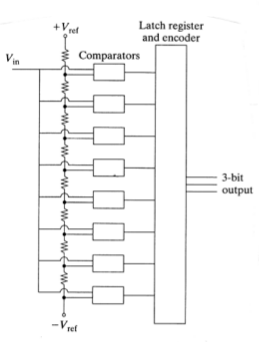
\includegraphics[scale=1]{./Immagini/ADCFlash.png}
\caption{Un ADC flash}
\label{fig:ADCFlash}
\end{center}
\end{figure}
\subsection{L'ADC multipasso}
Si pu\`o ottenere un buon compromesso tra velocit\`a e potenza utilizzando un ADC multipasso.
Questi dispositivi utilizzano dei convertitori ADC flash in cascata e si basano su una serie di scale di espansione:
una serie di moduli sincronizzati suddividono in segnale in modo sempre pi\`u fine al proseguire della digitalizzazione, 
ad esempio il primo modulo digitalizza il segnale su 3 bit, il secondo modulo considera la differenza tra il segnale originale e quello digitalizzato e la ridigitalizza
su una scala pi\`u fine e si procede fino ad una digitalizzazione soddisfacente.\\
Per esempio supponendo di avere in ingresso un segnale da 3.5V il primo ADC potrebbe produrre un segnale digitale corrispondente a 3V, il secondo
si occuperebbe di digitalizzare gli 0.5V rimanenti.\\
Dal punto di vista dell'elettronica, il segnale viene ricevuto e sdoppiato, una parte viene ritardata e l'altra viene digitalizzata, un amplificatore
esegue la differenza tra i segnali e lo manda al modulo successivo, lo schema si trova in figura~\ref{fig:ADCMultipasso}.
\begin{figure}[htbp]
\begin{center}
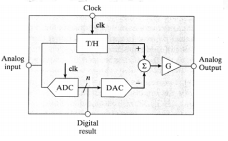
\includegraphics[scale=1]{./Immagini/ADCMultipasso1.png}\\
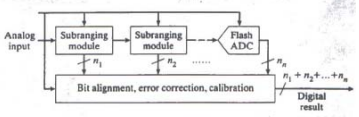
\includegraphics[scale=1]{./Immagini/ADCMultipasso2.png}
\caption{Schema di ADC Multipasso}
\label{fig:ADCMultipasso}
\end{center}
\end{figure}
Questi dispositivi hanno una velocit\`a nell'ordine dalle decine alle centinaia di MHz, ma richiedono una potenza minore (dalle decine a centinaia di mW)
e hanno DNL inferiori (nell'ordine di 0.5 LSB).
\section{Filtraggio e formatura del segnale digitale}
Quando si effettua un filtraggio di un segnale analogico, il segnale in uscita pu\`o essere visto come un integrale di convoluzione
tra la funzione di risposta del filtro e il segnale in ingresso:
\begin{equation*}
V'(t) = \int_{t-L}^t V(t') H(t-t') dt'
\end{equation*}
con $L$ durata del filtro\footnote{\`E interessante interpretare questo integrale come il prodotto di spettri di Fourier del segnale in ingresso e della funzione di risposta del filtro}.\\
Per un segnale digitale, questo integrale diventa una sommatoria:
\begin{equation*}
V'(j) = \sum_{i=j-L}^j V(i)H(j-i)
\end{equation*}
Supponiamo di voler implementare un filtro digitale, un metodo di calcolo della sommatoria \`e dato dal filtro a scorrimento, figura~\ref{fig:filtroScorrimento}.
In questi filtri, ogni passo di sovrapposizione da un $j$ in sequenza.
\begin{figure}[htbp]
\begin{center}
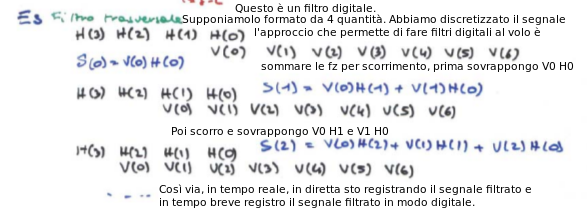
\includegraphics[scale=0.80]{./Immagini/FiltroScorrimento.png}
\caption{Funzionamento matematico di un filtro a scorrimento trasversale}
\label{fig:filtroScorrimento}
\end{center}
\end{figure}
In questo modo il tempo di filtraggio \`e breve e pu\`o essere effettuato in tempo reale, in quanto il segnale filtrato viene calcolato al volo.\\
Utilizzando questa tecnica sul rumore posso fare dei filtri adattivi per rimuoverlo, allo stesso modo \`e possibile realizzare filtri per pile-up facendoli variare
in base al rate.
\section{Analisi della forma dell'impulso}
La forma dell'impulso \`e in grado di contenere informazioni sul tipo di particella incidente, sull'interazione che ha generato l'impulso e sulla posizione spaziale dell'evento.
Queste tipo di elaborazioni sono molto impegnative computazionalmente, per questo devono essere fatte offline (ovvero in un secondo momento) su segnali digitalizzati e memorizzati.
\subsection{Ristabilimento della linea di base}
Se l'impulso viene digitalizzato \`e possibile campionare la linea di base per poter correggere di volta in volta l'impulso;
questa operazione richiede che per un certo lasso di tempo non avvengano eventi, per cui se si vuole campionare il pi\`u possibile
la linea di base per correzioni, \`e necessario trovare un compromesso con il rate di interazioni.
\subsection{Deconvoluzione di impulsi di pile-up}
Se ho un impulso digtalizzato posso utilizzare un programma di analisi degli impulsi per riconoscere ed eseguire la deconvoluzione degli impulsi di pile-up.
Queste operazioni possono essere fatte interpolando i segnali, in quanto dopo la formatura si ha una espressione analitica per interpolare il segnale.
Chiaramente queste operazioni possono essere fatte unicamente offline e con un campionamento molto spinto.
\section{Estrazione di informazioni temporali}
Ci sono misure in cui \`e importante estrarre il momento di arrivo dell'impulso.
La precisione di questa misura dipende dal rivelatore (raccolta delle cariche libere) e dalla catena elettronica (ad esempio range dinamici ampii possono essere problematici).\\
Le \textbf{unit\`a di trigger} si occupano di produrre un impulso logico ogni qual volta venga discriminato un segnale, questi dispositivi sono soggetti a due problemi (figura~\ref{fig:timeJitter}):
\begin{itemize}
\item \textbf{Time jitter}, ogni segnale ha fluttuazioni casuali nel livello e nella forma dell'impulso dovuti, ad esempio, al rumore oppure a tempi diversi di raccolta delle cariche
che portano segnali legati a eventi identici ad avere istanti di trigger diversi. 
Per ridurre questo problema \`e necessario porre il livello di trigger in regioni dove la pendenza \`e massima, per cui \`e meno sensibile a fluttuazioni.
\item \textbf{Amplitude e rise time walk}, la variabilit\`a nel ampiezza massima del segnale (\textit{amplitude walk}) porta ad istanti diversi di trigger,
lo stesso pu\`o accadere per segnali che variano la loro forma. (\textit{time walk}).
Questi problemi si riducono in portata se si abbassa il livello di trigger.
\end{itemize}
\begin{figure}[htbp]
\begin{center}
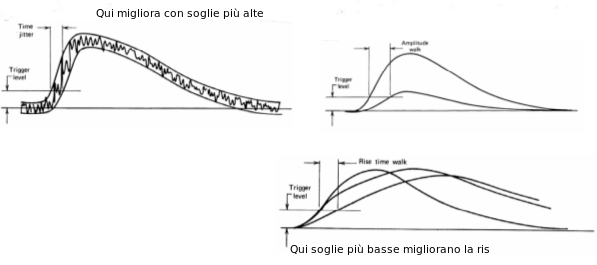
\includegraphics[scale=0.70]{./Immagini/TimeJitter.png}
\caption{Time jitter, amplitude walk e rise time walk}
\label{fig:timeJitter}
\end{center}
\end{figure}
\subsection{Leading edge trigger}
Il leading edge trigger fissa un livello di trigger e produce un impulso logico quanto il segnale supera tale livello, questa tecnica di triggering funziona abbastanza bene se i segnali non hanno un'ampiezza troppo variabile.
Il time jitter ci porta ad alzare il livello di trigger, l'amplitude walk ad abbassarlo: \`e presente un ottimo per soglie intorno al 10-20\% del segnale.
\subsection{Trigger sull'istante di crossover dello zero}
Se un segnale \`e bipolare, l'istante di passaggio del livello zero non \`e dipendente dall'ampiezza dell'impulso.
Per questi segnali \`e possibile eseguire un trigger sul momento del crossover, questa tecnica riesce a risolvere bene il problema dell'amplitude walk,
ma amplifica quello del time jitter.\\
Questa tecnica \`e utilizzabile anche sugli scintilllatori, sottoponendo il segnale anodico ad una singola linea di ritardo, purch\`e la forma
degli impulsi non vari molto.
\subsection{Constant fraction timing}
Se il range dinamico dell'impulso \`e ampio, ci si pu\`o svincolare dall'ampiezza dell'impulso eseguendo il trigger su frazioni $f$ dell'ampiezza massima;
in questo modo, a parit\`a di forma viene risolto il problema dell'amplitude walk.\\
Il constant fraction timing viene effettuato in questo modo (fig~\ref{fig:CFT}):
\begin{enumerate}
\item Il segnale viene sdoppiato
\item Una copia viene invertita e ritardata di un tempo maggiore del tempo di salita
\item L'altra copia viene moltiplicata per un fattore $f$ (quindi attenuata)
\item I segnali vengono sovrapposti e il trigger viene posto sull'istante di zero crossover
\end{enumerate}
\begin{figure}[htbp]
\begin{center}
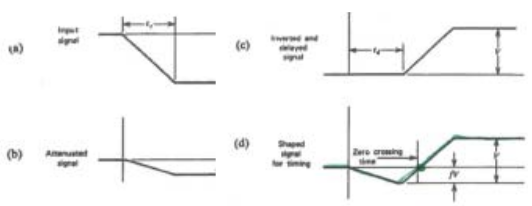
\includegraphics[scale=0.8]{./Immagini/CFT.png}
\caption{Elaborazione di un segnale per il CFT}
\label{fig:CFT}
\end{center}
\end{figure}
Essendo una tecnica basata sul zero crossover, soffre di problemi legati al time jitter, tuttavia risulta un'alternativa migliore in presenza di range dinamici ampii.
\subsection{ARC timing}
L'ARC (Amplitude and Rise time Compensation) timing viene utilizzato in quei rivelatori dove la forma ed il risetime variano, questo accade sopratutto nei rivelatori HPGe.
In questo tipo di timing si suppone che almeno la parte iniziale dell'impulso sia costante e si esegue il trigger sulla parte iniziale dell'impulso.\\
Un sistema ARC esegue queste operazioni(~\ref{fig:ARC}):
\begin{enumerate}
\item Sdoppia il segnale
\item Una copia viene ritardata di un tempo molto inferiore a quello di salita
\item L'altra copia viene invertita ed attenuata
\item I segnali vengono sommati per effettuare un trigger sullo zero crossover
\end{enumerate}
Questo tipo di trigger non compensa l'amplitude walk.
\begin{figure}[htbp]
\begin{center}
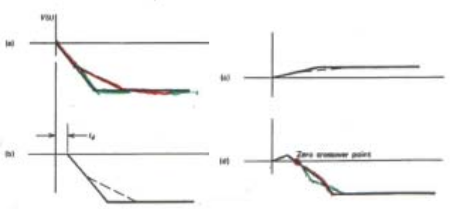
\includegraphics[scale=1]{./Immagini/ARC.png}
\caption{ARC timing}
\label{fig:ARC}
\end{center}
\end{figure}
\subsection{ELET timing}
L'ELET (Extrapolated Leading Edge Trigger) si basa sull'estrapolazione del fronte di salita utilizzando una parte che si suppone essere lineare e costante,
anche questa tecnica viene utilizzata su segnali di forma variabile (sempre HPGe).
Una coppia di discriminatori a soglia con rapporto tra le soglie fissato misurano l'intervallo di tempo tra i due punti ed estrapolano all'indietro il punto di inizio
del segnale.
La misura dell'intervallo di tempo viene effettuata con un TAC (Time to Amplitude Converter).
\subsection{FPET timing}
FPET (First PhotoElectron Trigger) esegue il trigger sul primo fotoelettrone in arrivo, pu\`o essere utilizzato negli scintillatori in condizioni di basso rumore sul fotomoltiplicatore.
\subsection{Confronto dei sistemi di timing}
II LET \`e il migliore per segnali con basso range dinamico e forma costante, il CFT \`e migliore per alti range dinamici e forma costante.
ARC e ELET vengono usati prevalentemente sul HPGe.
\section{Spettroscopia temporale}
\subsection{Spettroscopia temporale con un TAC}
Utilizzando un TAC e un MCA \`e possibile eseguire una spettroscopia temporale, in quanto il TAC produce un impulso proporzionale all'intervallo di tempo.\\
La risoluzione temporale del sistema cos\`i realizzato pu\`o essere misurata sdoppiando e ritardando un segnale che successivamente viene posto in ingresso al TAC.
Un sistema ideale mostrera una larghezza di un bin, nella realta si vedr\`a una regione gaussiana, la cui FWHM sar\`a la risoluzione.\\
Supponiamo di avere una sorgente che emette due quanti in coincidenza rivelati da due dispositivi su due rami diversi, eseguendo una spettroscopia temporale ci\`o che si osserver\`a nell'MCA sar\`a dato dalla sovrapposizione
di due grafici (fig~\ref{fig:spettroCoincidenze}):
\begin{itemize}
\item Un picco centrato in $t_f$ (tempo di ritardo di uno dei due rami) la cui area sar\`a il numero di coincidenze prompt. 
La FWHM indicher\`a la risoluzione del sistema. 
Se i due rami della catena elettronica sono simmetrici, allora il picco osservato sar\`a simmetrico, altrimenti si vedranno asimmetrie.
Ad esempio se il secondo ramo (che fa da stop) ha problemi di amplitude walk, si osserver\`a un'asimmetria verso la coda, in quanto l'amplitude walk ritarder\`a l'arrivo del segnale di stop.
\item Un fondo continuo, dovuto a coincidenze casuali. Se i rate di rivelazione dei due rami, $r_1$ e $r_2$, sono molto inferiori rispetto al reciproco della durata di tempo massima
misurabile dal TAC, allora si osserver\`a un fondo costante di concidenze casuali. \\
Per dimostrarlo calcoliamo la probabilit\`a che si verifichi una coincidenza casuale al tempo $T$.
Supponiamo che ci sia stato un evento nel rivelatore 1, la probabilit\`a che avvenga un evento all'istante $T$ \`e data dalla probabilit\`a
che non avvengano eventi fino al temo $T$ per la probabilit\`a che avvenga un evento tra il tempo $T$ e $T+dT$:
\begin{equation*}
P(T) = e^{-T \, r_2} \, r_2 \, dT
\end{equation*}
Moltiplicando per $r_1$ si ottiene il tasso di coincidenze casuali ad un tempo fissato:
\begin{equation*}
r_{12}=r_1\, r_2 \, e^{-T \, r_2} \, dT
\end{equation*}
Se $r_2\ll T^{-1}$ allora $T\,r_2 \ll 1$ e il termine esponenziale pu\`o essere approssimato a 1 ottenendo:
\begin{equation*}
r_{12} = r_1 \, r_2 \, \Delta T
\end{equation*} 
dove si \`e sostituito $dT$ con $\Delta T$ larghezza di un picco del MCA.
\end{itemize}
\begin{figure}[htbp]
\begin{center}
	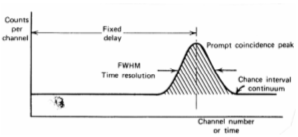
\includegraphics[scale=1]{./Immagini/SpettroCoincidenze.png}
\caption{Analisi con MCA di coincidenze}
\label{fig:spettroCoincidenze}
\end{center}
\end{figure}
Per migliorare il rapporto tra l'area del picco e del fondo si pu\`o migliorare la risoluzione temporale del TAC e introdurre una selezione delle ampiezze.
Avere un'attivit\`a $n$ minore della sorgente pu\`o aiutare dato che le coincidenze casuali vanno come $n^2$ e le reali come $n$.
\subsection{Spettroscopia temporale con un'unit\`a di coincidenza}
Un'unit\`a di coincidenza produce un impulso logico, ogni qualvolta riceve in ingresso due impulsi entro un tempo $\tau$, esso rappresenta, quindi, una sorta di SCA sul tempo.\\
Questo dispositivo, insieme ad un dispositivo per produrre ritardi variabili, pu\`o essere usato per eseguire spettroscopie temporali.
Riprendendo il sistema a due rivelatori precedente, sottoponiamo un segnale ad un ritardo fissato $t_f$ e l'altro ad un ritardo variabile $t_v$.
Se $\tau = \frac {\Delta T} { 2}$ (l'intervallo registrato \`e $(-\tau , +\tau)$) allora l'unit\`a di coincidenza esegue lo stesso numero di conteggi di un canale dell'MCA:
variando $t_v$, l'unit\`a segnaler\`a le coincidenze temporali con tempo $t_f - t_v$.\\
In questi sistemi \`e importante impostare bene $\tau$, se esso \`e troppo grande esso contegger\`a troppe coincidenze casuali, se \`e troppo piccolo sar\`a difficile vedere
il picco delle coincidenze casuali. 
Il valore migliore risulta $\tau = L/2$ con $L$ larghezza alla base del picco, scegliere dei $\tau$ sopra questa media porter\`a a dei plateau di coincidenze casuali (fig.~\ref{fig:plateau}),
andare sotto ridurr\`a l'altezza del picco, rendendolo pi\`u difficile da individuare.
\begin{figure}[htbp]
\begin{center}
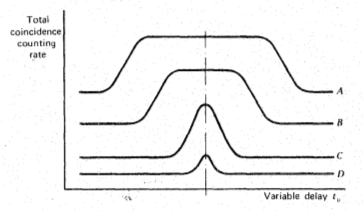
\includegraphics[scale=1]{./Immagini/Plateau.png}
\caption{Esempi di spettri ottenuti con questa tecnica al variare di $\tau$}
\label{fig:plateau}
\end{center}
\end{figure}
Normalmente non si prende il valore minimo di $\tau$, in quanto possono capitare derive temporali che modificano il rate di eventi;
per questo esso viene preso un po' pi\`u grande del minimo.
\subsection{Correzione delle coincidenze casuali}
Nel caso di coincidenze casuali a due la correzione del fondo \`e piuttosto semplice in quanto esso \`e piatto e vale $2 \tau \, r_1 \, r_2$.\\
La situazione diventa pi\`u complicata per le coincidenze multiple, per esempio per le coincidenze a tre esiste un fondo piatto $2 \tau  \, r_1 \, r_2$,
tuttavia esiste anche la possibilit\`a di avere una coincidenza reale a due con una casuale. 
Quest'ultima \`e difficilmente valutabile e spesso si ricorre ad un'analisi sperimentale per determinare il fondo.
\subsection{Determinazione di $\tau$}
Il fondo delle coincidenze a due pu\`o essere utilizzato per determinare $tau$ usando, ad esempio, due sorgenti scorrelate ben schermate oppure utilizzando
una sola sorgente che emetta quanti non in coincidenza.\\
Un'altra possibilit\`a pu\`o venire dal misurare la larghezza del plateau, in questo caso \`e utile una sorgente che emetta un'elevata quantit\`a di 
radiazione in coincidenza.
\subsection{Misura di coincidenze ritardate}
Supponiamo di avere una sorgente che emetta due quanti in sequenza passando per uno stato metastabile a vita media inferiore alla risoluzione temporale del sistema.
In questo caso vedremo un picco gaussiano di coincidenze vere con una coda sulla destra di tipo esponenziale, da essa si pu\`o estrarre le informazioni di interesse sulla vita dello stato.\\
Questa misura pu\`o essere effettuata utilizzando un MCA, oppure utilizzando un'unit\`a di coincidenza che effettui una scansione della regione di interesse.\\
Un'altra di questo tipo viene effettuata con la spettroscopia T.O.F. di neutroni, misurando l'intervallo di tempo tra l'istante di produzione e di arrivo
dei neutroni ad un rivelatore, si pu\`o misurare la loro energia.
\subsection{Misure di attivit\`a}
Supponiamo di avere una sorgente che emette 2 quanti $q_1$ e $q_2$ di radiazione in coincidenza con attivit\`a $S$ senza alcuna correlazione angolare, inoltre immaginiamo di avere un rivelatore
sensibile solo ai quanti di tipo $q_1$ e un altro rivelatore sensibile solo ai quanti di tipo $q_2$.\\
Siano $\epsilon_1$ e $\epsilon_2$ le relative efficienze (comprensive di fattori angolari, di efficienze di interazione e altro), allora i tassi di rivelazione saranno:
\begin{gather}
r_1 = \epsilon_1 \, S\\
r_2 = \epsilon_2 \, S
\end{gather}
mentre il tasso di coincidenze vere rivelate sar\`a:
\begin{equation*}
r_{t} = \epsilon_1 \, \epsilon_2 \, S
\end{equation*}
Chiamando $r_{ch}$ il tasso di coincidenze casuali, allora il tasso di coincidenze totali misurate sar\`a
$r_{12} = r_{t} + r_{ch} = \epsilon_1 \, \epsilon_2 \, S + r_{ch} $, risolvendo il sistema si trova:
\begin{equation*}
S = \frac{r_1 \, r_2}{r_{12}-r_{ch}}
\end{equation*}
ovvero l'attivit\`a della sorgente.\\
Questo questo metodo si pu\`o misurare con una accuratezza del 1\% le attivit\`a delle sorgenti senza avere rivelatori che coprano l'intero angolo solido;
inoltre se un rivelatore copre l'angolo solido, allora si pu\`o rinunciare al bisogno di avere radiazione scorrelata angolarmente.\\
Questo metodo tipicamente viene applicato su coincidenze $\beta-\gamma$.
Un rivelatore sensibile solo ai $\gamma$ pu\`o essere ottenuto interponendo un assorbitore di $\beta$ prima del rivelatore, tuttavia un rivelatore
sensibile ai $\beta$ misura sempre qualche fotone, in questo caso \`e necessario cercare di selezionare le energie.\\
Coincidenze $\gamma - \gamma$ sono ancora pi\`u difficili, in quanto anche selezionando le energie, il fondo per l'effetto Compton da sempre parecchi problemi.
\section{Moduli per misure temporali}
\subsection{Moduli di trigger}
I moduli di trigger andrebbero posti subito dopo il rivelatore, tuttavia questo comporta un peggioramento della FWHM.\\
Per questo se si \`e interessati a mantenere l'informazione sull'energia \`e meglio metterlo dopo lo stadio di preamplificazione, dove,
se la salita dell'impulso \`e veloce, l'informazione temporale viene preservata.\\
L'eccezione viene dagli scintillatori, dove, utilizzando una resistenza di carico da 50 $\Omega$ (che genera segnali pi\`u veloci), il segnale all'anodo pu\`o essere utilizzato per misure temporali, 
mentre utilizzando una resistenza pi\`u grande tra l'ultimo dinodo e l'anodo si pu\`o ottenere un segnale a coda lunga con informazioni sull'energia.\\
Altri moduli di trigger possono richiedere una formatura (ad esempio lo zero crossover), in questo caso vanno posti dopo l'amplificatore,
talvolta i moduli di trigger sono integrati in discriminatori o SCA, in modo da non sacrificare troppo l'informazioni sull'ampiezza.
\subsection{Unit\`a di coincidenza}
Se si \`e interessati ad una misura di sovrapposizione degli impulsi, allora il $\tau$ di coincidenza deve essere pari alla larghezza dell'impulso, mentre
se il circuito \`e sensibile al fronte di salita dell'impulso, allora il $\tau$ pu\`o essere scelto liberamente in base alle necessit\`a.\\
Spesso questi dispositivi possiedono pi\`u ingressi (da 1 a 4) che possono essere attivati o disattivati a seconda delle necessit\`a (concidenze a 2, a 3,...);
uno di questi ingressi a volte funge da anticoincidenza, per inibire il dispositivo quando necessario.
\subsection{TAC}
Questo dispositivo viene utilizzato insieme ad un MCA e produce un segnale lineare proporzionale all'intervallo di tempo tra due segnali di start e stop.
In questi dispositivi \`e fondamentale la linearit\`a, essa pu\`o essere misurata sdoppiando segnali e sottoponendoli a linee di ritardo.\\
Esistono TAC di due tipi:
\begin{itemize}
\item \textbf{A sovrapposizione}, il TAC riceve in ingresso due impulsi logici standard e misura l'area di sovrapposizione dei due segnali di start e stop.
Se essi sono in perfetta coincidenza allora gli impulsi si sovrapporranno perfettamente, altrimenti l'area sar\`a proporzionale all'intervallo di tempo: un integratore misura quest'area e d\`a l'informazione.
Questi dispositivi sono veloci nella misura, ma hanno problemi di linearit\`a e precisione, per cui vengono utilizzati in caso di alti rate.
\item \textbf{A start-stop}, in questi dispositivi i segnali di start e stop iniziano e interrompono l'accumulo di carica a corrente costante su un condensatore.
In questo modo la tensione ai capi sar\`a linearmente proporzionale al tempo, ottenendo un'ottima linearit\`a.
\end{itemize}
\subsection{TDC, Time to Digital Converter}
Non \`e molto sensato dover produrre un impulso lineare per poi digitalizzarlo, per questo esistono dispositivi che producono direttamente impulsi digitali.
In questi moduli viene prodotta un gate della durata dell'intervallo, questo gate controlla l'uscita di impulsi di clock a frequenza costante.\\
La frequenza massima attuale \`e di 1 GHz, per cui si pu\`o avere una precisione massima di 1 ns. 
Questo risulta problematico per impulsi brevi (a 20 ns, l'errore \`e del 5\%), per questo spesso i TDC sono corredati con dilatatori di impulsi
che interpolano e dilatano l'impulso temporale.
\subsection{Sistemi di ritardo}
Utilizzando cavi coassiali di diversa lunghezza \`e possibile realizzare sistemi di ritardo nella scala dei ns, tuttavia sopra i 100 ns questo sistema non \`e utilizzabile.
Per ritardi nei $\mu$s si possono utilizzare cavi coassiali con materiali speciali, tuttavia devono essere usati solo per portare segnali a bassa frequenza,
in quanto i segnali ad alta frequenza vengono fortemente distorti.
Spesso questi sistemi sono integrati in amplificatori per mettere a punto sistemi basati sulla temporizzazione.\\
Per ritardare gli impulsi logici poich\`e non si ha informazioni contenute nella forma si possono usare altri sistemi.
Uno di questi \`e basato sulla discriminazione di una rampa: l'impulso da ritardare avvia la salita di una rampa, quando essa supera un livello di discriminazione
viene prodotto un segnale logico in uscita, variando il livello si possono ottenere i ritardi desiderati.
\subsection{Amplificatori a banda larga e filtri temporali}
Talvolta pu\`o essere fondamentale mantenere l'informazione temporale, in questi casi \`e utile riuscire a mantenere il segnale inalterato nella forma
dopo lo stadio di amplificazione.
Un amplificatore a banda larga esegue questa operazione, amplifica semplicemente il segnale senza effettuare alcuna formatura.
Questo modulo \`e utile ad esempio con l'uscita anodica di un fotomoltiplicatore.\\
Se invece si necessita di una formatura minimale, allora si pu\'o utilizzare un filtro temporale, esso esegue un formatura con tempi
caratteristici inferiori ai comuni amplificatori, mantenendo cos\`i inalterata l'informazione temporale a costo di un rapporto segnale-rumore peggiore.
\section{Pulse Shape Discrimination e Rise Time Discrimination}
La forma dell'impulso \`e in grado di contenere informazioni come il tipo di particella che ha interagito con il rivelatore oppure la raccolta delle cariche.
Queste informazioni possono essere ottenute attraverso la PSD o la RTD.
La prima risulta efficace su segnali lineari veloci (come gli impulsi anodici), la seconda \`e equivalente alla PSD sugli impulsi lenti, come quelli del PRE.\\
La PSD pu\`o essere utile in questi casi:
\begin{itemize}
\item	Discriminazione del fondo $\gamma$ negli scintillatori organici se usati come rivelatori di neutroni veloci
\item Riconoscimento del tipo di particella in alcuni scintillatori inorganici
\item Discriminazione tra particelle a range breve e lungo nei contatori proporzionali (tipo le camere a gas)
\item Eliminazione di impulsi spuri nel Ge e nel Si
\item Reiezione di pile-up, osservando le deformazioni
\end{itemize}
Esistono due approcci possibili, uno \`e basato sul sentire le differenze nel rise time, l'altro \`e basato sull'integrazione del segnale in diversi punti:
\begin{itemize}
\item Con due discriminatori a soglie fissate si possono produrre segnali di start e stop per un TAC e osservare la velocit\`a del fronte di salita
\item Si pu\`o rendere il segnale bipolare e poi utilizzare un crossover. 
L'istante di crossover non dipende dall'ampiezza, bens\`i solo dalla forma, per cui misurando l'intervallo di tempo tra un punto fissato (ad esempio il 10\% del fronte di salita)
e lo zero crossover con un TAC ed eseguendo la spettroscopia con un MCA si pu\`o determinare il tipo di particella (fig~\ref{fig:PSD}). 
Un SCA pu\`o essere utilizzato per selezionare il tipo di particella di interesse.
\item Si pu\`o integrare il segnale in due istanti diversi ed eseguire il rapporto dell'integrazione. Questo rapporto non dipende dall'ampiezza e da un
fattore di discriminazione della forma.
\end{itemize}
Si introduce la figura di merito:
\begin{equation*}
M = \frac{X}{W_a + W_b}
\end{equation*}
questo fattore da una misura della qualit\`a della separazione dei segnali ottenuta con il PSD, esso dipende dal range dinamico dei segnali,
per la definizione di $X$, $W_a$ e $W_b$ vedere figura~\ref{fig:PSD}.
\begin{figure}[htbp]
\begin{center}
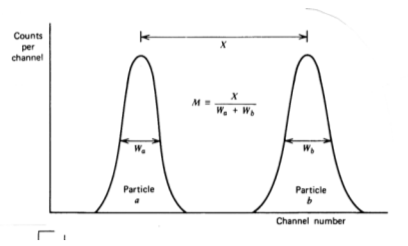
\includegraphics[scale=1]{./Immagini/PSD.png}
\caption{PSD con zero crossover e figura di merito}
\label{fig:PSD}
\end{center}
\end{figure}
\chapter{MultiChannel Analyzer}
\section{Analisi degli impulsi con un MCA}
Lo spettro \`e una funzione $\frac{dN}{dH}$, nella realt\`a \`e nella forma $\frac{\Delta N}{\Delta H}$, con $\Delta H$ larghezza di un canale.\\
In passato l'analisi di uno spettro avveniva con un SCA le cui soglie venivano regolate di volta in volta, adesso questi studi vengono effettuati
utilizzando degli SCA in parallelo, ovvero con un MCA.
Lo svantaggio nell'uso di un MCA \`e nella possibile sovrapposizione di canali, oppure nella non perfetta uniformit\`a delle loro larghezze.
\section{Caratteristiche di un MCA}
\subsection{Canali richiesti}
Il numero di canali richiesti per un'analisi \`e importante, esso \`e determinato da tre fattori:
\begin{itemize}
\item Risoluzione del rivelatore
\item Binning del software di analisi
\item Conteggi per canale
\end{itemize}
Lo spettro discreto deve essere il pi\`u possibile vicino a quello continuo, tuttavia aumentare troppo il numero di canali
riducendo la loro larghezza ha degli inconvenienti: essendo la statistica a singolo canale di tipo poissoniana, restringere un canale
riduce il numero di conteggi, quindi la loro fluttuazione cresce (va come l'inverso del numero di conteggi), nascondendo l'eventuale
presenza di picchi secondari deboli (fig.~\ref{fig:binningMCA}). 
\begin{figure}[htbp]
\begin{center}
	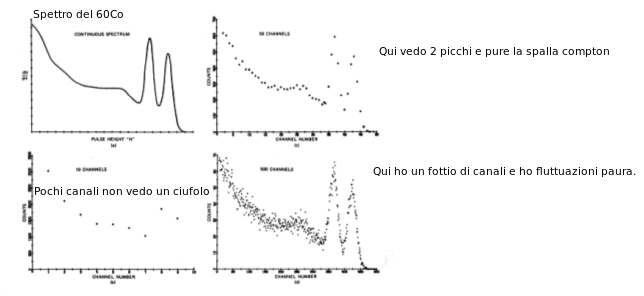
\includegraphics[scale=0.7]{./Immagini/BinningMCA.png}
\label{fig:binningMCA}
\end{center}
\end{figure}
In genere i software di analisi richiedono 9-12 canali corrispondenti alla FWHM\%, per cui a una FWHM\% del 10\% corrispondono circa 100 canali nel picco.
\subsection{Calibrazione e linearit\`a}
In un MCA ideale, la retta di calibrazione canale-tensione \`e perfettamente lineare; nella realt\`a questo non accade, in generale \`e possibile
aggiungere degli offset per fare in modo che al canale 0 corrispondano tensioni non nulle.
La pendenza della retta di calibrazione tensione-canale \`e dipendente dall'elettronica, ad esempio cambiare l'amplificazione modifica la sua pendenza,
se il dispositivo \`e lineare, sono sufficienti due punti per ottenere il fit, nella realt\`a questa calibrazione viene fatta con molti pi\`u punti, 
in modo da testare la linearit\`a.\\
Ho due tipi di non-linearit\`a: quella integrale, che mi da la massima deviazione tra la tensione sperimentale del canale e la curva best fit;
quella differenziale, ottenuta sottoponendo l'MCA ad una distribuzione uniforme in ampiezza di impulsi ed acquisendone lo spettro, in modo
da determinare disuniformit\`a nella larghezza del canale.
Un buon MCA ha deviazioni di non linearit\`a differenziali nel \%.
\begin{figure}[htbp]
\begin{center}
	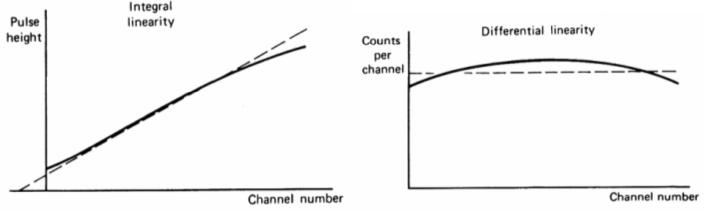
\includegraphics[scale=0.60]{./Immagini/NonLinearitaMCA.png}
\caption{Curve di non linearit\`a in un MCA}
\end{center}
\end{figure}
Una possibile sorgente di non linearit\`a viene anche dall'ADC che come gi\`a visto pu\`o avere larghezze dei canali non omogenee.
\section{Componenti di un MCA}
Il cuore di un MCA \`e dato dall'ADC (non di tipo flash o multipasso), esso riceve il segnale e ne digitalizza il picco.
Prima di un ADC \`e presente un circuito di ingresso, esso ha lo scopo di trattenere in memoria l'impulso e trasmetterlo all'ADC per tutta la durata della conversione,
un gate blocca tutti gli impulsi per la durata della conversione e da informazioni sul tempo morto del MCA.
All'uscita del ADC \`e presente una memoria formata da tante regioni quanti i canali del ADC e che conteggia il numero di segnali ricevuti, in genere
il numero di bit per area di memoria \`e tale da poter tenere un numero di conteggi nell'ordine dei $10^9$.\\
Spesso all'ingresso di questa catena viene posizionato un SCA, esso viene utilizzato per selezionare impulsi contenuti in una particolare regione,
in questo modo \`e possibile ridurre il tempo morto del MCA non facendo digitalizzare gli impulsi non utili.\\
Al termine della catena \`e presente un terminale che visualizza i dati e li salva, spesso si utilizza un PC. 
Il PC, tuttavia, \`e un ambiente rumoroso, per cui \`e necessario avere un architettura dedicata oppure posizionare l'ADC esternamente al dispositivo.
\section{Dettagli sul ADC}
Come detto prima, ADC flash e multipasso hanno problemi di non linearit\`a, per questo si usando altri tipi di ADC.
\subsection{ADC con rampa lineare (Wilkinson)}
In questo ADC all'arrivo del segnale viene prodotta, mediante una corrente costante ed un condensatore, una rampa lineare.
Un impulso di gate rimane attivo per il periodo di tempo in cui la rampa \`e sotto la tensione in ingresso e viene utilizzato
per pilotare degli impulsi di clock.
Il numero di impulsi di clock indica quanto tempo il gate \`e rimasto attivo e quindi il numero di impulsi prodotti sono una digitalizzazione
del segnale.
Chiaramente in questo ADC il tempo di digitalizzazione dipende dall'ampiezza dell'impulso ed \`e nell'ordine di multipli del reciproco della frequenza di clock,
frequenze tipiche sono nel centinaio di MHz (10 ns per canale), ma ha il vantaggio di avere un'ottima linearit\`a.
\subsection{ADC ad approssimazioni successive}
Questo ADC si basa su una sorta di ricerca dicotomica, un comparatore compara il segnale con la tensione corrispondente al 
primo bit pi\`u significativo del ADC. 
Se \`e maggiore allora il bit pi\`u significativo viene posto a 1 e si sottrae la tensione corrispondente al segnale originale, altrimenti esso viene posto a 0.
Il segnale viene quindi passato ad uno stadio che esegue lo stesso lavoro con il secondo bit pi\`u significativo e cos\`i via.\\
Il vantaggio di questo dispositivo \`e che ha tempi di conversione costanti (se ho 10 bit faccio 10 passaggi con tempi nei microsecondi), tuttavia ha non linearit\`a maggiori.
\subsection{Il principio della scala che scorre}
Questo metodo permette di ridurre le DNL, una tensione casuale viene aggiunta al segnale che viene successivamente digitalizzato.
La stessa tensione aggiunta viene anch'essa digitalizzata e poi sottratta al output del primo segnale.
Supponendo che alla tensione casuale corrisponda il canale M e che le fluttuazioni sulle larghezze dei canali siano casuali, questo metodo
migliora le uniformit\`a dei canali di un fattore $\sqrt{M}$.\\
Il problema principale di questo metodo \`e che se si suppone di dare pi\`u volte lo stesso segnale in ingresso esso pu\`o corrispondere a canali differenzi
con un peggioramento della risoluzione del MCA (senza il metodo avremmo tutto nello stesso canale, in proporzione alla sua DNL).\\
Un altro problema \`e dato dall'utilizzo di due ADC diversi: se i fattori di scala non sono bene accoppiati possono apparire strutture artefatte nello spettro.
\section{Tempo morto degli MCA (NON HO CAPITO IL METODO HARMS)}
Le sorgenti principali di tempo morto all'interno di un MCA sono due: l'ADC e la memorizzazione.
\`E importante misurare il tempo morto per poterlo successivamente correggere.\\
Per MCA con ADC Wilkinson il tempo morto segue la relazione:
\begin{equation*}
\tau = \frac{N}{\nu}  + B
\end{equation*}
con $N$ canale dell'impulso, $\nu$ frequenza del clock del ADC e $B$ tempo di memorizzazione.
In genere il tempo morto non dovrebbe superare il 30-40\% del tempo totale, altrimenti si possono osservare deformazioni dello spettro.\\
Gli MCA possiedono delle componenti che si occupano di misurare il tempo morto del dispositivo osservando la presenza del gate; questi misuratori sono affidabili purch\'e il tempo morto
non sia troppo elevato, altrimenti \`e necessario ricorrere ad altri metodi.\\
Un metodo \`e utilizzare un impulsatore per produrre impulsi artificiali nel PRE che verranno successivamente formati ed acquisiti.
Nel MCA ci si aspetter\`a di osservare un picco artificiale di una cerca area, osservando il rapporto tra gli impulsi acquisiti e gli impulsi prodotti si pu\`o determinare
il tempo morto; gli impulsi non devono essere prodotti troppo frequentemente e talvolta \`e preferibile utilizzare una produzione casuale.
Questo metodo \`e buono se lo spettro del MCA non ha derive nel guadagno o variazioni nei rate di misura, altrimenti pu\`o incorrere in problemi.\\
Un metodo suggerito da Harms \`e quello di produrre impulsi per un tempo di clock fissato.
\`E possibile determinare quando un impulso \`e stato perso esternamente (quindi dedurre il tempo morto),
in questo caso il tempo morto verr\`a compensato dando all'impulso successivo peso doppio.
Osservando lo spettro prodotto da tali impulsi \`e possibile determinare eventuali derive nello spettro. 
In caso di alti rate, il metodo pu\`o essere esteso conteggiando gli impulsi persi e aumentando del relativo fatto il peso dell'impulso successivo.
\section{Stabilizzazione dello spettro}
Eventuali derive dello spettro possono deformare i picchi, rendendo difficili le analisi spettrali.
Le cause di queste derive sono molteplici: variazioni di temperatura, di tensione, di guadagno, del tasso di conteggi (soprattutto negli scintillatori).\\
Gli stabilizzatori di spettro si occupano di percepire tali derive e correggere lo spettro di conseguenza. 
Una tecnica utilizzata \`e quella di porre due SCA simmetrici rispetto ad un picco e conteggiare il numero di impulsi, in assenza di derive il conteggio
sar\`a simmetrico, altrimenti sar\`a sbilanciato verso una coda, permettendo di misurare e correggere derive nel guadagno;
questa tecnica pu\`o essere applicata digitalmente utilizzando due Range Of Interest (ROI) nello spettro del MCA.
Questa tecnica pu\`o essere utilizzata ogni tot impulsi e correggendo di conseguenza, il problema \`e che statisticamente gli spettri sono sempre asimmetrici,
per cui ci sar\`a sempre una correzione nel guadagno, peggiorando la FWHM del picco. 
Tuttavia, se le fluttuazioni statistiche sono piccole, questo effetto pu\`o essere trascurato.\\
\`E inoltre possibile correggere offset utilizzando due picchi all'inizio e alla fine dello spettro.\\
Gli impulsi di test possono venire da una sorgente, oppure da un impulsatore, tuttavia quest'ultimo permette di testare unicamente l'elettronica, ma non lo scintillatore.
Utilizzare una sorgente pu\`o comportare del fondo indesiderato.
\subsection{Riallineamento dello spettro}
Un modo per risolvere il problema della deriva dello spettro \`e suddividere la misura in misure pi\`u brevi.
Il problema, comunque, rimane in quanto per avere una statistica maggiore pu\`o essere utile unire nuovamente gli spettri.
Questi spettri avranno un binning e una calibrazione diversa di volta in volta.\\
Il primo passo per affrontare il problema \`e quello di utilizzare pi\`u picchi per spettro, in modo da poter calibrare i singoli spettri e riportarsi sulla scala delle energie.
A questo punto \`e necessario utilizzare un binning comune in energia, per cui \`e necessario effettuare un rebin degli istogrammi per renderli tutti uniformi.\\
Supponiamo di voler rebinnare una regione di $M$ canali, se essi sono piccoli \`e possibile interpolarli con una polinomiale di grado $M-1$ per ottenere lo spettro continuo.
A questo punto, eseguendo il rapporto tra le aree sottese dalla polinomiale nel bin finale e quello originale, \`e possibile suddividere i vari bin sulla base del rapporto ed ottenere un buon rebinnaggio dei dati.
Questo metodo, tuttavia, fa perdere la statistica poissoniana dei singoli bin.
\section{Analisi degli spettri}
\subsection{Deconvoluzione e ricostruzione dello spettro reale}
Quando misuriamo uno spettro quello che viene osservato non \`e il vero spettro, in quanto l'elettronica risponde in modo diverso a seconda degli impulsi,
in particolare lo spettro osservato pu\`o essere scritto come:
\begin{equation*}
\frac{dN}{dH} = \int S(E) R(H,E) dE
\end{equation*}
dove $S(E)$ \`e lo spettro reale, mentre $R(H,E)$ \`e la funzione di risposta ovvero la probabilit\`a che un quanto di energia $E$ produca un impulso di ampiezza $H$.\\
Se supponiamo di avere una sorgente ad energia fissata, allora lo spettro reale \`e una delta di ampiezza $S_0$ e l'espressione precedente risulta:
\begin{equation*}
\left.\frac{dN}{dH}\right|_{E=E_0} = S_0 \, R(E_0,H)
\end{equation*}
Nel caso di un MCA si lavora con spettri discreti, quindi l'integrale diventa una sommatoria:
\begin{equation*}
N_i = \sum_{j} S_j R_{ij}
\end{equation*}
con $N_i$ numero di conteggi al canale i-esimo, $S_j$ ampiezza dello spettro (quindi l'intensit\`a di radiazione) all'energia j-esima, $R_{ij}$ matrice di risposta del sistema.\\
Lo spettro reale \`e chiaramente un continuo, ma dato che lo vediamo discreto, possiamo discretizzarlo in $L$ intervalli;
allora se conosco $R_{ij}$ posso risolvere il sistema associato e trovare $S_j$: avendo M canali, quindi M equazioni, il sistema \`e risolvibile per $L\le M$,
effettuando cos\`i la \textbf{deconvoluzione dello spettro}.
Se $R(H,E_0) = R_0 \delta (H-H_0)$ allora la matrice \`e diagonale ed esiste una corrispondenza biunivoca tra gli spettri, ma questo non capita sempre.\\
La tecnica della deconvoluzione possiede diversi problemi: inanzitutto non \`e possibile conoscere con precisione $R_{ij}$ in quanto non \`e possibile provare
la risposta ad ogni singola energia; inoltre anche conoscendo tutte le energie esistono problemi di natura statistica legati alla varianza di un singolo bin e
al fatto che le condizioni di lavoro possono cambiare.
Per questi motivi non \`e possibile conoscere con precisione lo spettro $S_j$, ma ci si accontenta di soluzioni approssimate,
un modo \`e quello di minimizzare la funzione di somma pesata dei residui:
\begin{equation*}
\epsilon^2 = \sum_i W_i \left(N_i - \sum_j S_j R_{ij}\right)^2
\end{equation*}
con $W_i$ pesi inversamente proporzionali all'incertezza del residuo. 
Per ridurre le incertezze si pu\`o eseguire del data smoothing, ovvero si pu\`o eseguire una media pesata dei canali con quelli adiacenti, scegliendo
come le dimensioni dell'intervallo di smoothing in modo che la funzione varii in modo brusco.\\
Le tecniche di deconvoluzione sono soprattutto usate nella spettroscopia di neutroni con rinculo di protoni e nei rivelatori a scintillazione o a germanio.
Se le energie da analizzare sono poche e ben note, allora si possono determinare i vari $R_{ij}$, altrimenti \`e necessario
usare calcoli e modelli analitici o sovrapporre curve sperimentali di funzioni di risposta.
\subsection{Stripping dello spettro}
Se lo spettro \`e formato da poche energie, posso pensare di decomporlo in sottospettri dovuti alla singola energia in base alle corrispondenti funzioni di risposta.
Supponiamo di avere uno spettro formato da 4 energie, si pu\`o ipotizzare che esso sia combinazione lineari di 4 funzioni di risposta:
per determinare il peso della funzione di risposta alla particella a energia pi\`u alta, si pu\`o considerare la porzione di spettro ad energia
maggiore, dove sono presenti unicamente le sue interazioni.
Estrapolando la funzione di risposta alle energie inferiori e sottraendo il suo contributo, si pu\`o procedere iterativamente fino a ridurre lo spettro
a 0, denudandolo.
\subsection{Analisi dei picchi}
Negli spettri $\gamma$ si ricorre raramente alla deconvoluzione, in quanto si osservano dei picchi caratteristici.
In presenza di tali picchi esiste una corrispondenza biunivoca tra spettro osservato e spettro della sorgente e non \`e necessario eseguire
deconvoluzioni\footnote{Se si volesse eseguire analisi del continuo Compton sarebbe invece necessario ricorrere a questa tecnica}.\\
Per localizzare i picchi bisogna tener conto di possibili picchi falsi ed eventuali doppietti: i primi sono riconoscibili in quanto hanno di solito
una FWHM molto minore, i secondi perch\`e sono invece con una FWHM maggiore.
In aggiunta, per la ricerca dei picchi si ricorre alla derivata seconda dello spettro, cercando regioni dove essa assume una variazione netta negativa.\\
Per determinare l'area sottesa dal picco \`e necessario inanzitutto rimuovere il fondo, successivamente si pu\`o ricorrere a due tecniche.
La prima consiste nel sommare tutti i canali del picco, scegliendo come regione di somma i canali significativamente maggiori del fondo e
assicurandosi si sceglierli in modo simmetrico rispetto al centro in base alla FWHM.\\
La seconda tecnica consiste nel fit della regione con una gaussiana sommata ad un esponenziale sulla sinistra che tenga conto degli eventi
con raccolta parziale della carica.
A questo punto \`e possibile determinare dal fit l'area, il canale centrale e la FWHM; le incertezze di questi tre parametri saranno:
\begin{itemize}
\item $\sqrt{A}$ per l'area
\item $\frac{\sigma}{\sqrt{A}}$ per il canale centrale
\item $\frac{W}{\sqrt{2A}}$ con $W=$ FWHM estratta dal fit
\end{itemize}

\chapter{Pile-up}
Il pile-up \`e un fenomeno di particolare importanza ad alti rate, avviene quando due impulsi dovuti a due eventi diversi interferiscono tra di loro
dando luogo ad impulsi dirtorti.
Il pile-up disturba gli spettri e le misure temporale degli impulsi.
Esistono pile-up di due tipi:
\begin{itemize}
\item \textbf{sulla discesa}, avviene durante il fronte di scarica del segnale ed \`e pi\`u probabile se esso \`e lento. Esso da luogo a impulsi
pi\`u alti del normale (coda destra della gaussiana) o pi\`u piccoli (se ho undershoot) del normale (coda sinistra della gaussiana). Pu\`o avvenire
anche a bassi rate.
\item \textbf{sulla salita}, avviene lungo il fronte di salita, da luogo ad impulsi pi\`u alti del normale (anche doppi). 
\end{itemize}
Questi problemi possono essere combattuti con una formatura adeguata, tuttavia formature troppo restrittive possono portare a problemi di rapporto segnale-rumore
oppure di deficit balistico.
\section{Stima del pile-up}
Per stimare il livello di pile-up posso ricorrere alla distribuzione degli intervalli di tempo:
ad ogni segnale posso associare un tempo caratteristico di larghezza $\tau$, per cui la probabilit\`a di non avere
pile-up con un rate $n$ di eventi \`e $P(t>\tau) = e^{-n\tau}$.
Quando si considera il pile-up \`e importante considerare che \`e un fenomeno che coinvolge due eventi, per cui per ogni evento di pile-up
due segnali sono stati rovinati: ad esempio, se su 100 segnali, ho il 10\% di probabilt\`a di avere pile-up, allora 10 segnali faranno
pile-up con altri 10, dando un'efficienza effettiva del 80\%.
Ad alti rate questa stima cade, in quanto posso avere pile-up tripli, quadrupli e chi pi\`u ne ha pi\`u ne metta.
\section{Reiezione del pile-up}
\`E possibile effettuare una reiezione degli impulsi di pile-up, tuttavia questa procedura aumenta il tempo morto, per cui sar\`a successivamente
necessario effettuare una correzione.
Gli impulsi di pile-up possono essere scartati mediante un PSD, in quanto gli impulsi avranno una forma diversa, oppure mediante un'analisi offline.
In alternativa \`e possibile sdoppiare il segnale in uscita dal PRE in due rami, uno lento che forma il segnale e uno veloce che produce un impulso logico;
un sistema verifica che al momento dell'arrivo del segnale formato non siano stati prodotti altri impulsi logici.
In assenza di ulteriori impulsi non sono giunti altri segnali che possono fare pile-up \`e l'impulso formato viene accettato; un sistema di questo tipo elimina pile-up entro la risoluzione temporale del ramo veloce.
\subsection{Correzione del numero di impulsi soggetti a pile-up}
Posso valutare il numero di impulsi che sono stati soggetti a pile-up utilizzando un impulsatore che produca impulsi di ampiezza tale da evitare
pile-up e che cadano in una regione dello spettro fuori dall'area di interesse per la misura.
L'impulsatore produce impulsi con rate fissato, per cui \`e possibile conoscere il numero di impulsi prodotti in un certo tempo, osservando l'area
del picco prodotto dall'impulsatore \`e possibile determinare la frazione di impulsi che non ha passato il sistema di reiezione del pile-up.
A questo punto, i segnali di interesse sono prodotti in modo piatto, si pu\`o supporre che la stessa frazione venga rigettata per pile-up
e si pu\`o correggere di conseguenza.
In realt\`a questo sistema andrebbe realizzato con generatore di impulsi casuale, tuttavia simulazioni MC hanno mostrato che se il rate
dell'impulsatore \`e inferiore al 10\% del rate di produzione dei segnali, allora i due sistemi sono equivalenti.
\section{Analisi statistica degli eventi di pile-up}
Poniamo $n$ il rate di conteggi reale e $m$ il rate di conteggi misurato.
\subsection{Rivelatore non paralizzabile}
In un rivelatore non paralizzabile vale:
\begin{equation*}
n = \frac{m}{1-m\tau}
\end{equation*}
\begin{equation*}
m = \frac{n}{1+n\tau}
\end{equation*}
In un tempo $\tau$ avvengono in media $n\tau$ eventi, la probabilit\`a che in un tempo $\tau$ facciano pile-up $x+1$ eventi vale:
\begin{equation*}
P(x) = \frac{(n\tau)^x e^{-n\tau}}{x!}
\end{equation*}
Se non voglio avere pile-up dovr\`o fare in modo di ridurre al minimo:
\begin{equation*}
P(0) = e^{-n\tau}
\end{equation*}
La media di eventi di pile-up in un tempo $\tau$ sar\`a:
\begin{equation*}
<x> = \sum_{i=0}^{\infty}(x+1) P(x) =\sum_{i=0}^{\infty}x \frac{(n\tau)^x e^{-n\tau}}{x!} + \sum_{i=0}^{\infty} \frac{(n\tau)^x e^{-n\tau}}{x!} = n\tau +1
\end{equation*}
ma poich\`e:
\begin{equation*}
<x> = \frac{n}{m} = n\tau +1
\end{equation*}
si pu\`o dire:
\begin{equation*}
m = \frac{n}{n\tau + 1}
\end{equation*}
coerentemente con la descrizione di rivelatore non paralizzabile precedente.
\subsection{Rivelatore paralizzabile}
Nel caso di un rivelatore paralizzabile:
\begin{equation*}
m = n e^{-n\tau}
\end{equation*}
La probabilit\`a di avere 0 conteggi in un $\tau$ \`e:
\begin{equation*}
P(0) = e^{-n\tau}
\end{equation*}
La probabilit\`a di avere 1 conteggio entro un $\tau$ \`e data dalla probabilit\`a di avere 0 conteggi entro $t$, averne uno entro $t$ e $t+dt$ e non averne pi\`u fino a $t+\tau$ (essendo paralizzabile adesso il rivelatore si sveglia a $t+\tau$ e non a $\tau$):
\begin{equation*}
P(1) = \int_0^{\tau} e^{-nt} n dt e^{-n\tau} = e^{-n\tau}(1-e^{-n\tau})
\end{equation*}
A questo punto \`e possibile calcolare la probabilit\`a di avere un pile-up triplo come la probabilit\`a di avere 0 eventi entro $t$, averne uno tra $t$ e $t+dt$ e poi averne un altro ancora entro $tau$, per cui ricorsivamente:
\begin{equation*}
P(2) = \int_0^{\tau} e^{-nt} n dt P(1) = e^{-n\tau} (1- e^{-n\tau} )^2
\end{equation*}
Induttivamente:
\begin{equation*}
P(x) =  e^{-n\tau} (1- e^{-n\tau} )^x
\end{equation*}
La media del numero di eventi in un tempo $\tau$ sar\`a:
\begin{equation*}
<x> = \sum_i=0^{\infty} (x+1) P(x) = e^{-n\tau}e^{2n\tau} = e^{n\tau}
\end{equation*}
Per cui si ottiene da $<x>=n/m$:
\begin{equation*}
m = n e^{-n\tau}
\end{equation*}
come ottenuto precedentemente.
\subsection{Spettri e tassi di pile-up}
Uno spettro pu\`o essere pensato come una combinazione lineare di spettri di zero pile-up, pile-up singolo, pile-up doppio e cos\`i via, pesati
per le singole probabilit\`a.
Se non utilizzo sistemi di reiezione del pile-up, allora il mio sistema \`e paralizzabile: se $\tau$ \`e la durata di un impulso, ciascun impulso
in pile-up allunga il tempo morto di $\tau$; se utilizzo reiezione, dipende dal tipo di sistema che utilizzo.\\
La frequenza di impulsi non soggetti a pile-up si trova da:
\begin{equation*}
f_e = \frac{P(0)}{<x>}
\end{equation*}
Nel caso non paralizzabile si trova ($n\tau \ll 1$):
\begin{equation*}
f_e = \frac{e^{-n\tau}}{n\tau + 1} \approx (1-n\tau)(1-n\tau) \approx 1-2n\tau
\end{equation*}
Nel caso paralizzabile si trova, sotto la stessa approssimazione:
\begin{equation*}
f_e = \frac{e^{-n\tau}}{e^{n\tau}} = e^{-2n\tau} \approx 1-2n\tau
\end{equation*}
Il tasso di eventi senza pile-up vale:
\begin{equation*}
r_{pf} = P(0) m  = e^{-n\tau} m
\end{equation*}
Per rivelatori non paralizzabili si ha:
\begin{equation*}
r_{pf} = P(0) \frac{n}{1+n\tau} 
\end{equation*}
Per rivelatori paralizzabili:
\begin{equation*}
r_{pf} = e^{-n\tau} n e^{-n\tau}
\end{equation*}
Esistono valori di n che massimizzano questi tassi, per i non paralizzabili vale $n = 0.618/\tau$, per i paralizzabili $n=0.5/\tau$.
Nei sistemi paralizzabili $m$ ha un proprio massimo, esso si vale $0.368/\tau$ se $n=1/\tau$, questo tasso porta ad avere una frequenza
di impulsi liberi da pile-up del $13.5\%$, mentre se massimizzo il rate di eventi pile-up free vale $36.8\%$, ovvero conto pi\`u eventi
liberi da pile-up, ma nel complessivo il 70\% degli impulsi totali \`e soggetto a pile-up.\\
Infine, il tasso di impulsi soggetti a pile-up se $\tau \ll n$  al primo ordine in $\tau$ vale:
\begin{equation*}
r_{pu} = m (1-P(0)) = m (1 - e^{-n\tau}) \approx m (n \tau) = n e^{-n\tau} (n\tau) \approx n^2 \tau 
\end{equation*}
\part{Tipi di rivelatori}
\chapter{Introduzione ai rivelatori di radiazione}
\section{Classificazione dei rivelatori}
I rivelatori vengono classificati in base a 3 fattori principali:
\begin{itemize}
\item La grandezza fisica da misurare
\item Tipo di radiazione da rivelare
\item Principio di funzionamento
\end{itemize}
\subsection{Tipo di grandezza fisica da misurare}
I rivelatori possono essere catalogati in base alla grandezza che devono misurare:
\begin{itemize}
\item Flusso di particelle
\item Conteggio di particelle
\item Misure di tempo
\item Misure di grandezze ''cinetiche``:
\begin{itemize}
\item Energia
\item Velocit\`a
\item Momento
\end{itemize}
\end{itemize}
In alcuni casi i rivelatori possono misurare pi\`u grandezze simultaneamente.
\subsection{Tipo di radiazione rivelata}
Alcuni tipi fondamentali sono:
\begin{itemize}
\item Spettroscopia $\alpha$
\item Spettroscopia $\beta$
\item Spettroscopia $\gamma$
\item Neutroni
\item Neutrini
\item $\gamma$ ed elettroni ad alta energia
\item Adroni ad alta energia
\end{itemize}
\subsection{Principio di funzionamento}
Esistono diversi principi:
\begin{itemize}
\item Ionizzazione di semiconduttori solidi cristallini o gas
\item Eccitazione atomica, scintillatori
\item Polarizzazione di materiali ed emissione Cherenkov, utilizzati per misure relativistiche (misure di fattori $\beta$ e $\gamma$ relativistici)
\item Misura di calore prodotto dal passaggio di una particella
\end{itemize}
\section{Misure in regime impulsivo}
I rivelatori a ionizzazione ed eccitazione possono essere utilizzati per effettuare misure di energia di singola particella.
Possiamo immaginare, infatti, che una particella di energia $E$ liberi una quantit\`a di carica $Q$ proporzionale all'energia,
raccogliendo questa carica su un condensatore si ottiene una tensione pari a $V_M = \frac{Q}{C}$.
Questo significa che vale $V \propto Q \propto E$ per cui $V = K \cdot E$, dove $K$ \`e una costante che pu\`o essere ricavata mediante il processo di calibrazione 
dell'apparato.
\subsection{La spettroscopia}
Quando eseguo una misura di energia sono interessato a studiarne la distribuzione, si parla in questo caso di \textbf{misure di spettroscopia}.
In pratica l'operazione che eseguo \`e quella di dividere lo spettro in una serie di intervalli uguali di dimensione $\Delta E$ e conteggiare il numero di particelle
di energia compresa tra $E$ e $E + \Delta E$.
\begin{figure}[htb]
\begin{center}
	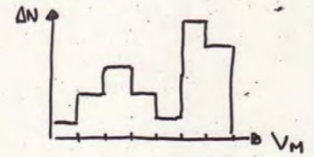
\includegraphics[scale=1]{./Immagini/Spettroscopia.png}
\caption{Esempio di spettro}
\end{center}
\end{figure}
Rimpicciolendo il numero di intervalli (in condizioni sperimentali questa suddivisione pu\`o essere spinta fino ad un certo punto) ottengo uno \textbf{spettro continuo} $\frac{dN}{dE}$.
A questo punto per conoscere il numero di particelle compreso tra due energie sar\`a sufficiente eseguire l'integrale dello spettro tra i due punti.
\subsection{Catena di lettura}
\begin{figure}[htbp]
\begin{center}
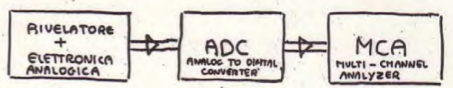
\includegraphics[scale=1]{./Immagini/CatenaDiLettura.png}
\caption{Catena di lettura}
\label{fig:CatLettura}
\end{center}
\end{figure}
La figura~\ref{fig:CatLettura} mostra la tipica catena di lettura di una spettroscopia:
\begin{enumerate}
\item Il \textbf{rivelatore}, tramite l'elettronica, produce un segnale proporzionale in tensione all'energia della particella, il segnale pu\`o essere soggetto ad un amplificazione
\item L'\textbf{Analog to Digital Converter} converte l'ampiezza del segnale ricevuto in una serie di impulsi logici, quantizzando l'ampiezza in una scala tra 1 e $2^n$ con $n$ numero di bit
\item Il \textbf{Multi Channal Analyzer} produce lo spettro, esso \`e formato da $2^n$ canali che conteggiano gli impulsi logici ricevuti, generando cos\`i lo spettro differenziale
\end{enumerate}
\section{Propriet\`a dei rivelatori}
Le caratteristiche fondamentali di un rivelatore sono:
\begin{itemize}
\item Efficienza
\item Risoluzione energetica
\item Risoluzione spaziale
\item Risoluzione temporale
\end{itemize}
\subsection{Efficienza}
L'\textbf{efficienza assoluta} di un rivelatore \`e definita come:
\begin{equation*}
\epsilon_{abs} = \frac{\text{\# di quanti rivelati}}{\text{\# di quanti emessi}}
\end{equation*}
L'efficienza assoluta dipende da diversi fattori:
\begin{enumerate}
\item Geometria del rivelatore
\item Attenuazione dal materiale
\item Efficienza di interazione
\item Efficienza di registrazione
\end{enumerate}
\subsubsection{Fattori geometrici}
Supponiamo di avere una sorgente che emette radiazione in modo isotropo, allora l'angolo solido coperto dal rivelatore risulta importante
per definire il \textbf{fattore geometrico}:
\begin{equation*}
G = \frac{\Omega}{4 \, \pi}
\end{equation*}
con $\Omega$ angolo solido coperto dal rivelatore:
\begin{equation*}
\Omega = \int_A dA \frac{\text{cos} \, \alpha }{r^2} 
\end{equation*}
con $A$ superficie del rivelatore e $\alpha$ angolo tra la normale della superficie $dA$ e la congiungente tra $dA$ e la sorgente.
\subsubsection{Attenuazione del materiale}
\`E necessario tener conto dell'effetto che il materiale ha sulla radiazione, in particolare possono esserci:
\begin{itemize}
\item Effetti di autoassorbimento della sorgente, ovvero la sorgente assorbe parte dell'energia che essa stessa emette (sorgenti spesse)
\item Effetti di assorbimento legati a materiale interposto tra sorgente e rivelatore, ad esempio dell'aria residua in casi di vuoto non ben fatto
\item Assorbimenti di energia nelle regioni di volume morto del rivelatore, ovvero regioni dove non vengono rivelati i depositi di energia da parte della radiazione.
Questo pu\`o accadere ad esempio nell'involucro del rivelatore.
\end{itemize}
\subsubsection{Efficienza di interazione}
Si definisce l'\textbf{efficienza di interazione} come:
\begin{equation*}
I = \frac{\text{\# di impulsi registrati}}{\text{\# di quanti di radiazione che incidono sul volume vivo}}
\end{equation*}
Per dei fotoni incidenti, valendo $n(x) = n_0 \, (1-\text{exp}(- \mu \cdot x))$ l'efficienza risulta:
\begin{equation*}
I = (1-\text{exp}(- \mu \cdot x))
\end{equation*}
Per le particelle cariche $I \approx 1$ in quanto \`e sufficiente una qualsiasi coppia elettrone-ione per avere una rivelazione.
\subsubsection{Efficienza di registrazione}
Viene definito come:
\begin{equation*}
R = \frac{\text{\# di impulsi registrati}}{\text{\# di interazioni}}
\end{equation*}
\subsubsection{Altre definizioni}
L'\textbf{efficienza intrinseca} indica l'efficienza del rivelatore indipendentemente dall'angolo solido coperto:
\begin{equation*}
\epsilon_{int} = \epsilon_{abs} \frac{4 \, \pi}{\Omega} = \frac{\epsilon_{abs}}{G}
\end{equation*}
L'\textbf{efficienza al picco}:
\begin{equation*}
\epsilon_{ip} = \frac{\text{\# di conteggi ad energia piena}}{\text{\# di quanti di radiazione che incidono sul rivelatore}}
\end{equation*}
\subsection{Risoluzione energetica}
Supponiamo di avere un rivelatore che emette radiazione ad energia $E$, osservando lo spettro differenziale prodotto dal MCA
si osserver\`a che esso non \`e formato da un'unica colonna, ma sar\`a formato da pi\`u colonne a distribuzione simil-gaussiana.
La \textbf{Full Width at Half Maximum} (FWHM) di questa distribuzione viene utilizzata per misurare la risoluzione energetica del dispositivo.
In particolare la FWHM pu\`o essere data in V o in eV, moltiplicando il voltaggio per il fattore di calibrazione.\\
Il deterioramento della risoluzione pu\`o essere dovuto a rumore sulla linea di base (fig.~\ref{fig:rumore}) o a fluttuazioni nella quantita di ionizzazione prodotta.
\begin{figure}[htb]
\begin{center}
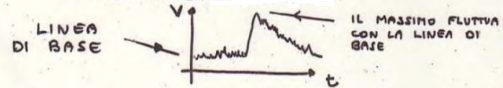
\includegraphics[scale=0.8]{./Immagini/Rumore.png}
\caption{Rumore sulla linea di base}
\label{fig:rumore}
\end{center}
\end{figure}
Altre cause del peggioramento della risoluzione possono essere trovate nella dipendenza dalla posizione della risposta del rivelatore e nella deriva temporale del fattore di calibrazione.
\subsubsection{Fluttuazioni nella generazione della carica}
Supponiamo di aver liberato $n$ portatori di carica, allora $Q = n \cdot q$ e $E = N \cdot \frac{Q}{C}$ per cui $E \propto n$,
poich\`e la ionizzazione \`e un processo statistica $n$ fluttua, le fluttuazioni di $n$ possono essere viste come un incertezza su $H$.\\
Cerchiamo di valutare quest'incertezza, il processo di ionizzazione \`e di tipo poissoniano:
\begin{equation}
P(n) = \frac{(N)^n \, e^{-N}}{n!}
\end{equation}
con $N$ numero di cariche mediamente liberate da una particella ad energia $E$ e $P(n)$ probabilit\`a di liberare $n$ cariche.
La varianza sar\`a $\sigma^2 = N$, se il numero di cariche liberate \`e sufficientemente elevato, la distribuzione pu\`o essere approssimata con una gaussiana.
Dato che $H = \frac{q \cdot n}{C}$ allora $\sigma_H = \frac{q}{C} \sigma_N = \frac{q}{C} \sqrt{N}$, per le gaussiane:
\begin{equation*}
\text{FWHM} = 2.35 \cdot \sigma_H 
\end{equation*}
mentre la risoluzione percentuale risulta:
\begin{equation*}
\frac{\text{FWHM}}{H_{max}} = \frac{2.35 \cdot \sigma_H}{H} = 2.35 \frac{1}{\sqrt{N}}
\end{equation*}
In realt\`a il processo non \`e puramente poissoniano, in quanto gli eventi non sono del tutto indipendenti, per cui vale:
\begin{equation*}
\sigma_{N}^2 = F \cdot N
\end{equation*}
con $F$ \textbf{fattore di Fano}.
\subsection{Risoluzione spaziale}
Si pu\`o ottenere della risoluzione spaziale usando rivelatori traccianti, rivelatori con elettrodi segmentati o matrici di rivelatori identici.
Si definisce \textbf{precisione spaziale} la precisione con la quale viene ricostruita la traccia lasciata dalla particella:
i punti della traccia possono essere interpolati linearmente per ottenere una traccia ben definita, la precisione viene calcolata come:
\begin{equation*}
\sigma^2 = \frac{\sum (x_{mis} - x_{interp}}{N-2}
\end{equation*}
$N-2$ \`e legato al fatto che 2 gradi di libert\`a vengono persi per via del fit lineare.\\
La \textbf{risoluzione spaziale} viene calcolata come la minima distanza tra due tracce risolte individualmente.
\subsection{Risoluzione temporale}
La \textbf{risoluzione temporale} \`e il minimo intervallo di tempo tra due eventi consecutivi che il rivelatore \`e in grado di distinguere,
corrisponde al \textbf{tempo morto} del rivelatore.
I fattori che incidono su questa caratteristica sono legati al metodo e fisica di rivelazione del dispositivo e alla strumentazione elettronica in lettura.
Se due eventi non possono essere risolti temporalmente allora pu\`o avvenire un \textit{pile-up}, questo pu\`o significare:
\begin{itemize}
\item un errato conteggio degli eventi
\item un errata valutazione dell'energia che pu\`o essere valutata come la somma delle due
\end{itemize}
\`E fondamentale riuscire a produrre delle correzioni a questo problema, prima \`e necessario distinguere tra due tipi di rivelatore: paralizzabile e non (figura~\ref{fig:tempoMorto}).
\begin{figure}[htbp]
\begin{center}
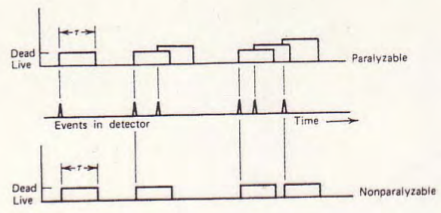
\includegraphics[scale=0.90]{./Immagini/TempoMorto.png}
\caption{Distinzione tra rivelatore paralizzabile e non.}
\label{fig:tempoMorto}
\end{center}
\end{figure}
Poniamo $n$ tasso di interazioni e $m$ tasso di rivelazioni, allora per un \textbf{rivelatore non paralizzabile} il tempo morto totale risulta
$\tau_{tot} = \tau \cdot m$, per cui il numero di interazioni reali avvenute durante questo lasso di tempo vale $n\cdot m \cdot \tau$.
Da ci\`o si deduce che in un rivelatore non paralizzabile il tasso di eventi persi vale $n \cdot (m\,\tau) = n - m$, in conclusione:
\begin{equation}\label{eq:rivnonpar}
n = \frac{m}{1-m\cdot \tau}
\end{equation}
Si osserva che nel caso di tassi $n$ molto elevati $m \approx \frac{1}{\tau}$.\\
Nel caso di un \textbf{rivelatore paralizzabile} la probabilit\`a che un intervallo sia lungo t \`e data dalla probabilit\`a che
in tale intervallo non avvenga alcun evento. 
Questa probabilit\`a \`e data dalla distribuzione di Poisson con $\lambda = n \cdot t$ e vale:
\begin{equation*}
P(0,t) dt = e^{-nt} dt
\end{equation*}
Normalizzando:
\begin{equation*}
P(0,t) dt  = n\,e^{-nt} dt
\end{equation*}
per cui la probabilit\`a che un intervallo di tempo morto sia pi\`u lungo di $\tau$ \`e:
\begin{equation*}
P(\tau) = \int_{\tau}^{\infty} P(t) \, dt = e^{-n \tau}
\end{equation*}
Per cui il tasso apparente $m$ risulta:
\begin{equation} \label{eq:rivpar}
m=n e^{-n\tau}
 \end{equation}
\subsubsection{Misura del tempo morto}
Una misura del tempo morto pu\`o essere ottenuta utilizzando una sorgente a vita media bassa, poniamo $n_b$ il tasso del fondo ambientale:
\begin{equation*}
n = n_0^{-\lambda t} + n_b
\end{equation*}
Se la sorgente ha vita media bassa allora $n_b \approx 0$:
\begin{equation*}
n = n_0^{-\lambda t}
\end{equation*}
Nel caso di un rivelatore paralizzabile da~\ref{eq:rivpar} si ha che:
\begin{equation*}
n = m \, e^{n\tau } = m \, \text{exp}(n_0 \, e^{-\lambda t})
\end{equation*}
introducendo questa espressione e applicando i logaritmi si ottiene:
\begin{equation} \label{eq:rivpartau}
\lambda t + \text{ln} m = - n_0 \tau e^{-\lambda t} + \text{ln} n_0
\end{equation}
Nel caso di un rivelatore non paralizzabile da~\ref{eq:rivnonpar} si ha:
\begin{equation} \label{eq:rivnonpartau}
m e^{\lambda t} = -n_0 \tau m + n_0
\end{equation}
Ponendo nelle equazioni~\ref{eq:rivpartau} e~\ref{eq:rivnonpartau} il lato sinistro come $y$ e $x = e^{\lambda \, t}$ 
dal coefficiente angolare \`e possibile ricavare $\tau$ e identificare il modello di rivelatore adatto.
\chapter{Scintillatori}
Gli scintillatori si basano sull'emissione luminosa da parte di atomi eccitati:
una particella ionizzante deposita la propria energia sul materiale causando una eccitazione atomica o molecolare e, in seguito,
emissione di radiazione luminosa.
Gli scintillatori hanno usi multipli:
\begin{itemize}
\item Spettroscopia $\gamma$
\item Calorimetria
\item Sistema T.O.F.
\item Sistema di trigger
\item Sistema di veto
\item Traccianti
\end{itemize} 
Possono essere divisi in due macrocategorie:
\begin{itemize}
\item Inorganici, caratterizzati da una buona resa in luce (e quindi una maggiore efficienza), ma anche pi\`u lenti
\item Organici, con una resa in luce minore, ma una maggiore velocit\`a
\end{itemize}
\section{Meccanismo di scintillazione}
\subsection{Scintillatori inorganici}
\begin{figure}[htb]
\begin{center}
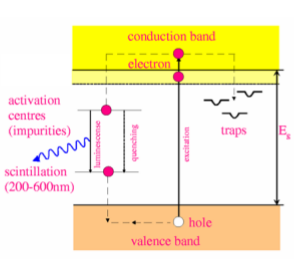
\includegraphics{./Immagini/LivelliEnergeticiScintillatore.png}
\caption{Livelli energetici in uno scintillatore inorganico}
\label{fig:livInorganico}
\end{center}
\end{figure}
La figura~\ref{fig:livInorganico} mostra il funzionamento di uno scintillatore inorganico.\\
In uno scintillatore organico per stimolare le attivazioni vengono introdotte delle impurezze, quando un elettrone viene portato
dalla banda di valenza a quella di conduzione entro qualche ns si ricombina con la lacuna emettendo radiazione.
Per via delle impurezze a volte accade che l'elettrone si vada a posizionare in un livello energetico dell'impurezza, questo
livello energetico ''trappola`` pu\`o richiedere tempi lunghi fino alle centinaia di ms per la diseccitazione. 
In questo caso avviene una fosforescenza.\\
Questi tipi di scintillatori hanno un elevato $Z$ e alta densit\`a, rendendoli adatti alla rivelazione di particelle cariche e raggi $\gamma$.
\subsection{Scintillatori organici}
\begin{figure}[htb]
\begin{center}
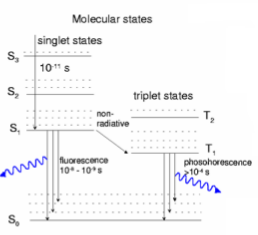
\includegraphics[scale=1.00]{./Immagini/LivelliEnergeticiScintillatoreOrganico.png}
\caption{Livelli energetici di uno scintillatore organico}
\label{fig:livOrganico}
\end{center}
\end{figure}
Gli scintillatori organici si basano sull'eccitazione di molecole di tipo organico, in particolare queste molecole sono caratterizzate
da orbitali molecolari di tipo $\pi$ tra le molecole di carbonio che possono essere stimolati per emettere luce nell'ultravioletto.\\
Posso avere scintillatori a monocristalli, liquidi o plastici a seconda dell'uso che si intende fare.\\
Il grande pregio di questo tipo di rivelatore sta nella velocit\`a di risposta che \`e nei ns.
Sono, inoltre, molto economici.
\section{Caratteristiche di uno scintillatore ideale}
\begin{enumerate}
\item Alta efficienza di scintillazione
\item Conversione lineare $S = E \cdot L$
\item Trasparenza 
\item Tempo di emissione breve
\item Buone propriet\`a ottiche e meccaniche. Buona maneggiabilit\`a.
\item Indice di rifrazione simile al vetro, per evitare riflessione totale.
\end{enumerate}
\subsection{Efficienza di scintillazione}
Uno scintillazione ideale dovrebbe avere un elevato $S$:
\begin{equation*}
S = \frac{L}{E} 
\end{equation*}
con $L$ energia luminosa e $E$ energia entrante.
Normalmente questo fattore \`e molto contenuto, nell'ordine del 10\%, per il NaI vale 12\% (il migliore).
Il resto dell'energia finisce in fononi e ionizzazione.\\
La \textbf{formula di Birks} (vale sono per gli scintillatori organici) afferma:
\begin{equation*}
\frac{dL}{dx} = \frac{S \frac{dE}{dx}}{1 + k_B \, \frac{dE}{dx}}
\end{equation*}
con $k_B$ costante di proporzionalit\`a di Birks.
Per le particelle $\alpha$ $\frac{dE}{dx}$ \`e molto grande per cui si ricava $\frac{dL}{dx} = \frac{S}{k_B}$, per gli elettroni
$\frac{dE}{dx}$ \`e piccolo per cui il termine al denominatore pu\`o essere approssimato a 1, ottenendo $L = S \cdot E$.\\
L'efficienza dipende dalla temperatura (fig~\ref{fig:traspInorganici}), dalle impurezze (per via del quenching) e si deteriora con il tempo.
\begin{figure}[htbp]
\begin{center}
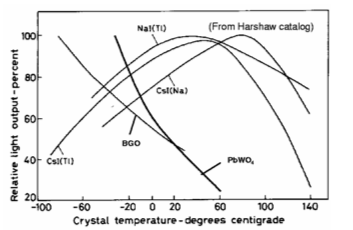
\includegraphics[scale=1]{./Immagini/TrasparenzaOrganici.png}
\caption{Andamento della trasparenza con la temperatura, esistono temperature ottimali.}
\label{fig:traspInorganici}
\end{center}
\end{figure}
\subsection{Linearit\`a}
La relazione $S = E \cdot L$ deve essere lineare, in particolare $S$ non dovrebbe dipendere dalla posizione dello scintillatore.
In generale $S$ dipende dalla particella, come si \`e visto dalla formula di Birks e per particelle che disperdono molta energia la relazione perde in linearit\`a:
per elettroni sufficientemente energetici (sopra il centinaio di keV) la relazione \`e lineare, per protoni o $\alpha$ non \`e lineare ad alte energie (si osservano
effetti di quenching tra molecole).
\subsection{Trasparenza}
\`E importante che lo spettro di assorbimento si sovrapponga il meno possibile con lo spettro di emissione, in modo da avere un materiale trasparente ai fotoni e
permettere ad essi di uscire dal materiale scintillante.
\subsection{Tempo di emissione}
Per avere un'elevata risoluzione temporale \`e necessario che la costante di tempo $\tau$ sia molto breve:
\begin{equation*}
I(t) = I_0 e^{-\frac{t}{\tau_0}} + I_1 e^{-\frac{t}{\tau_1}} - I_0 e^{-\frac{t}{\tau_p}}
\end{equation*}
con $\tau_0$ tempo di scintillazione, $\tau_1$ tempo di fosforescenza e fluorescenza ritardata e $\tau_p$ tempo per il popolamento dei livelli eccitati.
\subsection{Proprieta ottiche e meccaniche}
Per propriet\`a ottiche si intende che la geometria dello scintillatore deve essere tale da avere una buona raccolta di luce, per questo \`e necessario
che i cristalli abbiano buone propriet\`a meccaniche: essi devono essere, infatti, di dimensioni e forma variabili secondo le necessit\`a.\\
Per quanto riguarda la maneggevolezza alcuni cristalli sono igroscopici, ovvero assorbono l'umidit\`a dell'aria, per questo devono essere isolati e sotto vuoto, e possono
essere fragili.
\section{La raccolta della luce}
Quando uno scintillatore emette luce, essa viene diffusa in modo isotropico, per questo motivo \`e importante avere un buon meccanismo di raccolta della luce.
Per evitare che la luce esca dal cristallo senza andare sul fotocatodo si usa il meccanismo della riflessione totale:
\begin{equation*}
\text{sin} \, \theta_c = \frac{n_1}{n_0}
\end{equation*}
Questo permette di avere minori perdite alla superficie (l'efficienza \`e sul 80\%) tuttavia rende difficoltosa la trasmissione del segnale al fotocatodo.
Per questo sulla superficie rivolta verso il fotocatodo viene posto un materiale di accoppiamento, ovvero un materiale a indice di rifrazione intermedio, come
del grasso ottico o del silicone.
Siccome il fotocatodo lavora con campi elettrici e magnetici intensi \`e necessario porlo ad una certa distanza dal cristallo, pe questo
\`e necessario guidare la luce verso il fotocatodo mediante l'uso di \textbf{guide di luce}, fibre a geometria cilindrica che trasportano la radiazione luminosa.
\section{Il fotocatodo}
Il fotocatodo ha il ruolo di emettere fotoelettroni quando fotoni di sufficiente energia incidono su di esso.
Questo dispositivo non \`e sensibile a tutta la radiazione luminosa: 
per ottenere l'emissione di un fotoelettrone \`e necessario che il fotone incidente
abbia energia sufficiente a portare un elettrone dalla banda di valenza del materiale alla
banda di conduzione ed a farlo uscire dalla superficie del fotocatodo (generalmente $E_{\gamma} > 2$ eV).
Per questo motivo il fotocatodo \`e in grado di rivelare solo una certa porzione dello spettro
luminoso, in genere a partire dal giallo-verde, in base al materiale che lo compone. \\
Per costruire i fotocatodi si utilizzano dei semiconduttori drogati ad affinit\`a elettronica negativa, ad esempio GaP drogato di tipo p con zinco.\\
Quando un elettrone viene portato in banda di conduzione, esso inizia ad eccitare i fononi del cristallo,
disperdendo la propria energia e raggiungendo (generalmente entro 1 ps) il fondo della banda.
Una volta che si trova in questo stato, l'elettrone impiega un tempo nell'ordine dei 100 ps per ricombinarsi con una
lacuna, tornando in banda di valenza.
L'energia sul fondo della banda di conduzione non \`e sufficiente per permettere agli elettroni di fuggire dal fotocatodo:
tra il materiale ed il vuoto esiste, infatti, una barriera di potenziale (detta affinit\`a elettronica) che impedisce agli elettroni di lasciare il semiconduttore.
Gli unici elettroni ad avere energia sufficiente per superare la barriera sono quelli che
hanno eccitato pochi fononi, per cui gli elettroni possiedono un tempo di 1 ps per lasciare il fotocatodo.
Questo tempo \`e molto breve e pone seri limiti allo spessore del materiale, in quanto gli elettroni possono percorrere poco spazio.
Per aumentare l'efficienza dei fotocatodi, essi vengono contruiti in modo da avere un'affinit\`a elettronica negativa e permettere agli elettroni sul fondo della banda di conduzione di avere energia sufficiente per fuggire.
Questo effetto viene ottenuto deponendo uno strato monoatomico di un materiale elettropositivo (ad esempio il cesio) sulla superficie del dispositivo:
poich\'e gli elettroni del cesio sono poco legati, essi vengono attratti dalle lacune del semiconduttore, ionizzando lo strato ed abbassando l'affinit\`a elettronica.
\subsection{Fabbricazione dei fotocatodi}
Esistono 2 categorie di fotocatodi, quelli opachi, con uno spessore maggiore della profondit\`a di fuga degli elettroni e quelli semitrasparenti.
In quelli opachi gli elettroni vengono prelevati dallo stesso lato in cui la luce incide sul materiale, in quelli semitrasparenti avviene l'opposto, in quanto la luce
riesce a raggiungere l'altro estremo del materiale.\\
Ad ogni modo \`e fondamentale che i fotocatodi abbiano uno spessore uniforme, per avere un estrazione uniforme indipendentemente dalla regione colpita dalla radiazione.
Esistono fotocatodi bialcalini o multialcalini a seconda della risposta alla radiazione che si desidera ottenere.
\section{Il fotomoltiplicatore}
\begin{figure}[htbp]
\begin{center}
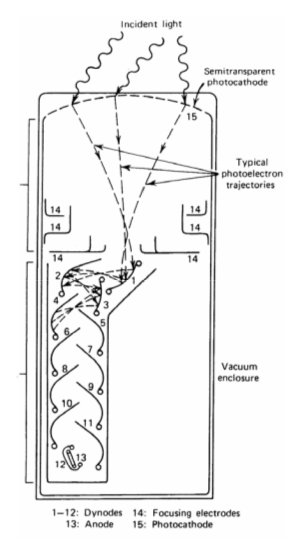
\includegraphics[scale=0.8]{./Immagini/Fotomoltiplicatore.png}
\caption{Schema di un fotomoltiplicatore}
\label{fig:fotomolt}
\end{center}
\end{figure}
Il rendimento quantico di un fotomoltiplicatore viene definito come:
\begin{equation*}
\text{Q.E.} = \frac{N_{pe}}{N_{fot}} \approx 20\% - 30\%
\end{equation*}
esso dipende dalla lunghezza d'onda del fotone incidente.
Un fotomoltiplicatore si basa sulla moltiplicazione di fotoelettroni attraverso stadi successivi chiamati \textbf{dinodi}.
Quando un fotoelettrone lascia il fotocatodo, esso viene accelerato da un potenziale verso i dinodi, l'urto con i dinodi libera della carica che
attraverso ulteriori urti viene moltiplicata e, infine, raccolta sull'anodo, producendo un segnale elettrico misurabile.
Tipicamente ogni urto con un dinodo porta ad un guadagno da 3 a 50 elettroni, il prodotto di tutti i guadagni da il guadagno globale.
Ad esempio 10 dinodi con guadagno $g=4$ moltiplicheranno di un fattore $G=4^{10}\approx 10^6$.\\
Di particolare importanza \`e il rumore termoionico dovuto ad emissioni termiche di elettroni da parte del fotocatodo:
a 300 K, $k_b T$ vale circa 25 meV, tuttavia per le code della distribuzione si ha che alcuni elettroni hanno un energia maggiore del lavoro di estrazione, 
causando falsi segnali.
Per questo motivo \`e necessario tenere il fotocatodo freddo, in genere per i semiconduttori si hanno dai 100 ai 10000 elettroni/cm$^2$ e s.\\
La \textbf{risoluzione energetica} \`e fortemente dominata dalla moltiplicazione al primo dinodo, dove gli elettroni sono pochi e 
$\frac{\sigma_E}{E} \propto \frac{1}{\sqrt{n}}$.
\subsection{I dinodi}
Supponiamo che un fotone liberi un elettrone e che esso sia accelerato da una differenza di potenziale di 100 V verso il primo dinodo.
Essendo il gap nell'ordine dei 2-3 eV, verranno eccitati circa 30 elettroni, di cui solo 4-5 usciranno dal dinodo per andare verso lo stadio successivo.
Aumentando il potenziale la quantit\`a di elettroni liberati cresce, tuttavia essi verranno liberati pi\`u in profondit\`a.
Per questo motivo esiste un valore ottimale per il potenziale di accelerazione.\\
In genere per i dinodi standard il valore di moltiplicazione \`e 5, per i materiali ad affinit\`a elettronica negativa si possono raggiungere fattori di moltiplicazione
pari a 20-30.
\section{Alimentazione del sistema a dinodi}
Chiaramente \`e necessario che la tensione dell'anodo sia maggiore di quella del fotocatodo, questo pu\`o essere ottenuto in due modi:
\begin{itemize}
\item fotocatodo a massa e anodo a tensione positiva
\item fotocatodo a tensione negativa e anodo a massa
\end{itemize}
Per alimentare i vari stadi di moltiplicazione \`e comodo usare un partitore resistivo (figura~\ref{fig:partitoreDinodi}).
\begin{figure}[htb]
\begin{center}
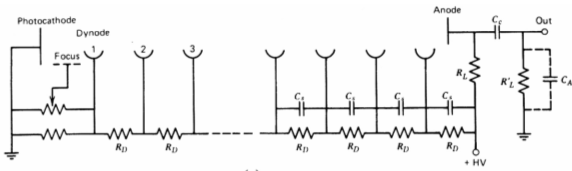
\includegraphics[scale=0.80]{./Immagini/PartitoreDinodi.png}
\caption{Esempio di partitore resistivo per i dinodi}
\label{fig:partitoreDinodi}
\end{center}
\end{figure}
Chiaramente un sistema di questo tipo porta ad avere delle correnti di fuga che per effetto Joule portano ad un aumento della temperatura del dispositivo.
Questa corrente, tuttavia, non pu\`o essere minimizzata troppo, in quanto deve essere maggiore della corrente di fotomoltiplicazione, in modo da mantenere
i potenziali tra i dinodi costanti.
Questo problema diventa rilevante negli ultimi stadi, dove il numero elevato di elettroni estratti porta a correnti di moltiplicazione intense.\\
Parlando quantitativamente si ha che in un tipico evento di scintillazione vengono liberati 1000 elettroni, un tipico fattore di moltiplicazione in un fototubo
\`e $10^6$, per cui si hanno $10^9$ elettroni nell'ultimo stadio di moltiplicazione.
Una tipica sorgente di laboratorio genera $10^5$ eventi ogni secondo, per un totale di $10^{14}\cdot 1.6 \cdot 10^{-19} = 16 \mu$A di corrente media.
Questa corrente media non provoca grandi riscaldamenti per effetto Joule, per cui una corrente di fuga di questo ordine non \`e tipicamente problematica;
tuttavia, questo ipotizza di avere un flusso continuo di elettroni, mentre nella realt\`a si hanno eventi impulsati di durata molto breve (nell'ordine del ns), per cui
la corrente massima diventa:
\begin{equation*}
i \asymp \frac{10^9 \cdot 10^{-19}}{10^{-9}} \asymp 100 \text{mA}
\end{equation*}
che \`e una quantit\`a notevole.
Per questo motivo ci si accontenta di usare una corrente nell'ordine della corrente media insieme a dei \textbf{condensatori di stabilizzazione}.
I condensatori di stabilizzazione vengono caricati dalla corrente di fuga nei momenti di quiete e servono a fornire la carica nella fase di fotomoltiplicazione.
Se i rate non sono troppo intensi il sistema \`e equivalente.
\section{Caratteristiche dei fototubi}
Le caratteristiche fondamentali sono:
\begin{enumerate}
\item Struttura, ogni fototubo ha una propria forma (circolare, esagonale,...)
\item Propriet\`a temporali, come tempo di risposta e risoluzione
\item Tensione e correnti massime, per determinare il guadagno massimo del dispositivo
\item Sensibilit\`a alla luce e alla potenza radiante (per usi in modo continuo)
\item Corrente di buio, ovvero la corrente che scorre nel dispositivo per catodo non illuminato
\item Linearit\`a del dispositivo, fortemente dipendente dalle fluttuazioni di tensione ai dinodi
\item Impulsi spuri e rumore associati ai fotomoltiplicatori
\item Disuniformit\`a nel fotocatodo, possono essere nella risposta, per via delle fluttuazioni di spessore, o nella raccolta al primo dinodo, 
che determina le fluttuazioni maggiori nella misurazione dell'energia.
\item Variazioni di guadagno in base al tasso di conteggi, per il motivo detto prima della compensazione della carica
\end{enumerate}
\section{Impulsi prodotti dal fototubo}
La legge di produzione dei fotoni \`e $I(t) = I_0$ exp$(-\lambda t)$ per cui la corrente di elettroni sar\`a
\begin{equation*}
 i(t) = i_0 \text{exp}(-\lambda t)
\end{equation*}
Da $\int_0^{\infty} i(t) dt$ si ricava
\begin{equation*}
i_0 = \lambda Q
\end{equation*} 
per cui $i(t) = \lambda Q$ exp$(\lambda t)$.\\
Il circuito di lettura del segnale pu\`o essere visto come un circuito RC, per cui la tensione sar\`a:
\begin{equation*}
V(t) = \frac{1}{\lambda - \theta} \frac{\lambda Q}{C} (e^{-\theta t} - e^{-\lambda t})
\end{equation*}
sovrapposizione degli effetti di resistenza e condensatore.\\
Se il tempo di produzione dei fotoni \`e molto inferiore del tempo di scarica RC del sistema, allora il segnale pu\`o essere approssimato come:
\begin{equation*}
V(t) \approx \frac{Q}{C}  (e^{-\theta t} - e^{-\lambda t})
\end{equation*}
Per cui il tempo caratteristico del fronte di salita sar\`a determinato da $\lambda$ mentre il tempo di discesa da $\theta$, il valore
massimo della tensione sar\`a $\frac{Q}{C}$.
Tipicamente per avere un segnale di questo tipo si utilizzano resistenze grandi e capacit\`a piccole, in modo da avere tempi lunghi di scarica e un 
valore di $\frac{Q}{C}$ grande.\\
Se il tempo di produzione dei fotoni \`e molto grande il segnale pu\`o essere approssimato come:
\begin{equation*}
V(t) \approx \frac{\lambda}{\theta}\frac{Q}{C} (-e^{-\theta t} + e^{-\lambda t}) 
\end{equation*}
Per cui, in modo opposto, i tempi di carica dipendono da RC, quelli di scarica da $\lambda$,
in questo modo dal decadimento del segnale \`e possibile ottenere informazioni sulla durata di produzione dei fotoni, per studi temporali.
Ad ogni modo a $\lambda$ e $\theta$ fissati, $V$ dipende linearmente da $Q$, per cui \`e possibile usare lo scintillatore per fare spettroscopia.
\section{Tempo di risposta e risoluzione temporale}
Un tipico fototubo a 14 dinodi ha una tensione totale di 2 kV, per cui la tensione tra una coppia di dinodi sar\`a di circa 150 V.
Supponendo che dopo un urto con un dinodo un elettrone abbia un energia di 0 eV, l'energia media di un elettrone in un fototubo sar\`a di 75 eV,
a cui corrisponde una velocit\`a di
\begin{equation*}
\beta^2  = 2 \bar{E}_k \approx \left(\frac{1}{60}\right)^2 
\end{equation*}
La lunghezza tipica di un fototubo \`e nella decina di cm, per cui i tempi di transito risultano nei 20 ns.\\
Le principali fluttuazioni di questo tempo sono date dalla distribuzione delle energie di uscita dei fotoelettroni dal fotocatodo (tra i 0 e i 2 eV),
quindi dalle fluttuazioni del tempo di transito dal fotocatodo al primo dinodo: esse sono nel decimo di ns ($0.2 - 0.3$ ns).
\section{Risoluzione energetica dello scintillatore}
Come si \`e detto prima una delle principali debolezze dello scintillatore \`e nella raccolta delle \textbf{cariche al primo dinodo}, dove si ha la maggiore fluttuazione
energetica in base ai fotoelettroni moltiplicati. 
Inoltre incidono sulla risoluzione: il \textbf{rumore elettronico}, le \textbf{disuniformit\`a del fotocatodo}, le \textbf{fluttuazioni nel guadagno del fotomoltiplicatore}
e la \textbf{non-linerarit\`a} della scintillazione.\\
La cariche prodotte dal fototubo sono il punto che incide maggiormente nella risoluzione, proviamo a fare un calcolo:
supponiamo che un fotone da 0.5 MeV incida su uno scintillatore con $S = 12\%$, questo significa che $L = 60$ keV.
Supponiamo che l'energia venga trasportata da fotoni a 3 eV, il numero totale di fotoni sar\`a 20000, per via per effetti di perdit\`a dell'informazione,
al fotocatodo ne arriveranno 15000. 
Un fotocatodo con efficienza quantica del 20\% produrr\`a 3000 elettroni; qui c`\`e la debolezza del sistema, infatti la produzione di elettroni \`e soggetta a questa
fluttuazione:
\begin{equation*}
\frac{\sigma_E}{E}  = \frac{\sigma_N}{N} = \frac{1}{\sqrt{3000}} \approx 1.8\%
\end{equation*}
Ovvero una FWHM di $2.35 \cdot 1.8 = 4.3 \%$.\\
La risoluzione dipende quindi da $\frac{1}{\sqrt{E}}$, in realt\`a sperimentalmente si vede che:
\begin{equation*}
R = \frac{(\alpha + \beta E)^{\frac{1}{2}}}{E}
\end{equation*}
con $\alpha$ e $\beta$ parametri sperimentali.\\
Altre cause di perdit\`a di risoluzione possono venire da \textbf{impurit\`a del cristallo}, da non uniformit\`a nella raccolta e conversione della luce,
nella non-linearit\`a della risposta legata alla distribuzione del numero di elettroni liberati ad energia fissata.
Un altro fattore \`e dato dalla perdit\`a di fotoni lungo il trasferimento verso il fotocatodo.\\
\textbf{Tipicamente la risoluzione viene quotata usando sorgenti a 662 keV o 1333 keV}.
\section{Rumore e impulsi spuri}
Rumore termoionico, fotoni ritardati dal cristallo e fotoni provenienti dai dinodi possono causare l'emissione di impulsi spuri.
Questi impulsi sono facilmente riconoscibili, in quanto dovuti a poche particelle, quindi a bassa energia:
filtrando gli impulsi piccoli posso, quindi, eliminarli.
Per ridurre questo problema posso ridurre la superficie del fotocatodo (riduce l'eff. termoionico), usare correnti di buio pi\`u piccole (per avere temperature minori),
Un'altra soluzione \`e raffreddare il fotocatodo, ma questo comporta la presenza di condensa e un aumento di radiazione uscente dal catodo che, per via del numero
elevato di elettroni, pu\`o comportare un'eccessiva distorsione del campo elettrico.\\
Altre sorgenti di impulsi spuri sono:
\begin{itemize}
\item Radioattivit\`a naturale
\item Radiazioni cosmiche
\item Gas residuo ionizzato, se la presenza diventa eccessiva \`e necessario cambiare il fototubo
\end{itemize}
\chapter{Spettroscopia $\gamma$}
A differenza delle particelle cariche, i fotoni possiedono diversi modi di interagire con la materia, noi non siamo in grado di rivelarli direttamente,
ci\`o che riveliamo \`e l'effetto prodotto sugli elettroni del materiale.
Per questo motivo un buon spettrometro $\gamma$ deve avere un'alta efficienza di conversione fotone-elettrone e deve essere in grado di rivelare efficientemente
tali particelle.
Un buon assorbimento di $e^{\pm}$ si ha con solidi di 1 cm di spessore.\\
Studiamo come reagisce il rivelatore ai tre effetti principali.
\section{Effetto fotoelettrico}
Nel caso di effetto fotoelettrico viene liberato un elettrone di energia $E = E_{\gamma} - E_b$, oltre a raggi X a cascata o elettroni Auger.
Se gli elettroni e i raggi X, tutti questi effetti vengono registrati dal rivelatore che, in conclusione, fornisce l'energia originaria del fotone.
Lo spettro quindi \`e dato da un picco detto anche \textbf{fotopicco}.
\section{Effetto Compton}
\`E il fenomeno prevalente nelle energie comprese tra 100 keV e 5 MeV in base al materiale.
L'energia ceduta agli elettroni dipende dall'angolo di scattering e va da un valore quasi nullo, per angolo nullo a
\begin{equation*}
E_{e}^{MAX} = h \nu \left(\frac{2\alpha}{1 + 2 \alpha} \right)
\end{equation*}
per un angolo di 180 gradi di scattering.\\
Per questo motivo lo spettro prodotto da effetto Compton \`e quello in figura~\ref{fig:spettroCompton} nel caso non venga assorbito il fotone
\begin{figure}[htbp]
\begin{center}
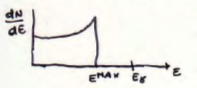
\includegraphics[scale=1]{./Immagini/SpettroCompton.png}
\caption{Spettro prodotto da un effetto Compton}
\label{fig:spettroCompton}
\end{center}
\end{figure}
\section{Produzione di coppie}
\`E il fenomeno dominante per alte energie, la coppia generata rilascia energia cinetica nel materiale e successivamente osserviamo l'annicilazione del positrone con
un elettrone.
Supponendo che tutta l'energia cinetica venga misurata posso osservare 3 picchi diversi a seconda dei fotoni da 511 keV assorbiti (figura~\ref{fig:spettroCoppia}.
\begin{figure}[htbp]
\begin{center}
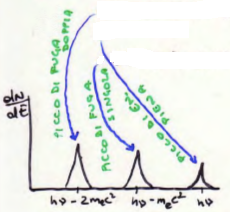
\includegraphics[scale=1]{./Immagini/SpettroCoppia.png}
\caption{Spettro prodotto dalla produzione di coppie}
\label{fig:spettroCoppia}
\end{center}
\end{figure}
Nel caso entrambi i fotoni da 511 keV vengano misurati allora osserviamo il \textbf{picco di energia piena}, tuttavia pu\`o accadere che uno dei due fotoni (o entrambi)
fuggano dal rivelatore, in questo caso osserviamo il \textbf{picco di fuga singola o doppia}.
Posso anche osservare casi intermedi, come degli effetti Compton e una successiva fuga.
\section{Funzione di risposta degli spettrometri $\gamma$}
\subsection{Caso del rivelatore piccolo}
Un rivelatore piccolo \`e un rivelatore sufficientemente grande da assorbire tutta l'energia cinetica degli elettroni, tuttavia di dimensioni inferiori al libero cammino
medio dei fotoni (che quindi non vengono, per la maggior parte, rivelati).
Lo spettro prodotto da un rivelatore di questo tipo \`e dato dal continuo del Compton, dal picco prodotto dall'effetto fotoelettrico e dal picco di doppia fuga.
\subsection{Caso del rivelatore grande}
Un rivelatore grande dovrebbe avere dimensioni nelle decine di cm, in questo caso tutti gli effetti e i fotoni secondari vengono rivelati, producendo solo 
picchi di energia piena e fotopicchi.
\subsection{Caso del rivelatore intermedio}
\`E il tipico caso di un rivelatore reale.
Posso avere picchi di energia piena insieme fughe di fotoni e scattering Compton multipli.
In questo caso la funzione di risposta del dispositivo viene simulata con metodi MonteCarlo.
Parametri importanti sono il rapporto tra il numero di picchi ad energia piena e il numero di eventi totali, il rapporto tra la fuga doppia e l'energia piena e
quello tra la fuga singola e l'energia piena.\\
La funzione di risposta di questi rivelatori ha delle complicazioni legate a:
\begin{itemize}
\item \textbf{Fuga di elettroni secondari}, che diventano importanti se il fotone \`e molto energetico o se il rivelatore \`e piccolo. Per via delle fughe l'energia misurata
	dal rivelatore sara inferiore rispetto a quella reale, peggiorando il rapporto energia piena/eventi totali.
\item \textbf{Fuga di fotoni da bremsstrahlung}, che diventa importante per elettroni molto energetici. L'energia irradiata in questo modo cresce come $Z^2$, anche in questo
	caso il continuo subisce un abbassamento di energia, oltre ad una distorsione nella forma.
\item \textbf{Fuga di raggi X caratteristici}, questo fenomeno diventa importante per fotoni ad energia minore (per via delle emissioni a cascata del fotoelettrico) e nei rivelatori con superfici
	molto pi\`u grandi rispetto al volume.
	Questo effetto produce dei picchi di fuga evidenti, in quanto i raggi X emessi hanno frequenze ben definite dai livelli energetici atomici.
\item \textbf{Radiazione secondaria prodotta vicino alla sorgente}, come la produzione di fotoni di annichilazione nell'ambiente in seguito ad un decadimento $\beta^+$.
	In questo caso viene osservato un picco a 511 keV (o a 1022 keV se il rivelatore \`e a pozzetto).
	Un altro effetto dovuto all'interazione con l'ambiente \`e la produzione di bremsstrahlung nei decadimenti $\beta^-$: in questo caso il continuo subisce un abbassamento in energia.
\item \textbf{Effetti dovuti a materiali esterni}, la radiazione prodotta dalla sorgente pu\`o interagire con l'ambiente e successivamente entrare nel rivelatore.
	Ad esempio un fotone potrebbe fare dello scattering Compton con l'ambiente e successivamente entrare nel dispositivo, in questo caso vedr\`o un aumento degli eventi nella
	regione a bassa energia. Un'altra possibilit\`a \`e un annichilazione con l'ambiente esterno, oppure la produzione di raggi X nell'ambiente esterno.
\item \textbf{Effetti dovuti alla somma di impulsi}, avviene nel caso di rate troppo intensi o nel caso di coincidenze, in questo caso il rivelatore non risolve
	temporalmente gli eventi e considera come un unico evento degli eventi distinti (\textit{pile-up}).
	In questo caso il rivelatore misurer\`a la somma delle energie e il conteggio degli eventi risulter\`a inevitabilmente falsato.
\end{itemize}
\begin{figure}[htbp]
\begin{center}
	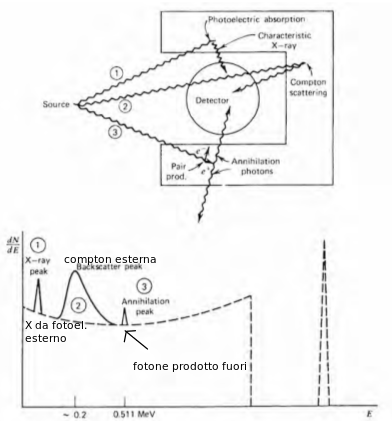
\includegraphics[scale=1]{./Immagini/EffettiGamma.png}
\caption{Possibili interazioni con l'ambiente che disturbano la misura}
\end{center}
\end{figure}
\section{Utilizzo di scintillatori come spettrometri $\gamma$}
La funzione di risposta degli scintillatori dipende dal tipo di cristallo usato, ad esempio il NaI ha un'ottima risoluzione e sezione d'urto
per effetto fotoelettrico, mentre il BGO (Bismuto-Germanio-Ossigeno) ha una sezione d'urto per fotoelettrico migliore (per cui ho meno picchi di fuga), 
ma una risoluzione peggiore in quanto ha un basso fattore di conversione energia-luce.\\
\begin{figure}[htbp]
\begin{center}
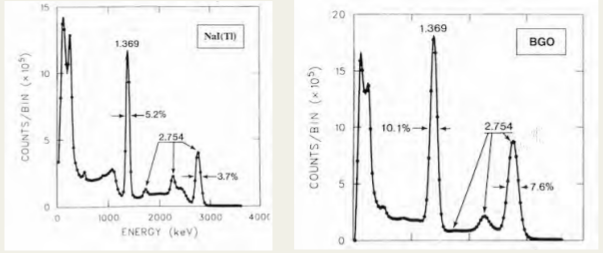
\includegraphics[scale=0.7]{./Immagini/ConfrontoRisposta.png}
\caption{Confronto delle funzioni di risposta dei due scintillatori.}
\end{center}
\end{figure}
La risoluzione \`e fondamentale per riconoscere picchi in quanto risoluzioni troppo basse potrebbero nascondere i picchi nel fondo.
\subsection{Risposta ai fotoni ad alta energia}
Quando l'energia dei fotoni aumenta (2-20 MeV), la sezione d'urto della produzione di coppie cresce.
Questo significa che verr\`a prodotta una coppia elettrone-positrone ad alta energia, quindi con una sezione d'urto per
bremsstrahlung maggiore.
Questo implica una maggiore perdit\`a alle superfici, per questo motivo all'aumentare dell'energia il picco di energia piena inizia a diminuire.
Inoltre, aumentando l'energia aumenta il numero di fotoelettroni che vengono prodotti nello scintillatore, poich\`e
FWHM $\propto N$ i picchi di energia piena, fuga singola e fuga doppia si allargano (figura~\ref{fig:confrontoAlteEnergie}).
\begin{figure}[htbp]
\begin{center}
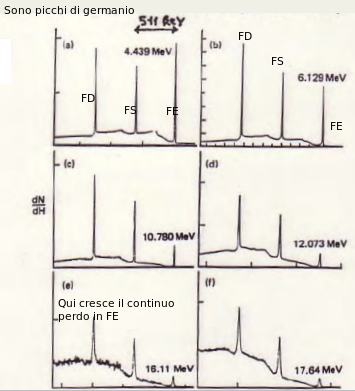
\includegraphics[scale=1]{./Immagini/ConfrontoAlteEnergie.png}
\caption{Spettro prodotto da germanio all'aumentare dell'energia}
\label{fig:confrontoAlteEnergie}
\end{center}
\end{figure}
\subsection{Linearit\`a della misura}
La relazione $L = S \cdot E$ deve essere il pi\`u possibile lineare, in quanto misuro con punti discreti, quindi devo
avere meno errori legati alla discretizzazione di una funzione continua.
La linearit\`a dipende dal tipo di particella e dall'energia: per elettroni la relazione ha una non-linearit\`a piuttosto ridotta;
per i fotoni, poich\`e la sequenza di interazioni che esso fa \`e diversa per ogni fotone che viene rivelato, esiste una maggiore
variabilit\`a, quindi le fluttuazioni sono maggiori, tuttavia comunque mantiene una certa linearit\`a per via del fatto che viene
misurato mediante interazioni con elettroni.
\begin{figure}[htbp]
\begin{center}
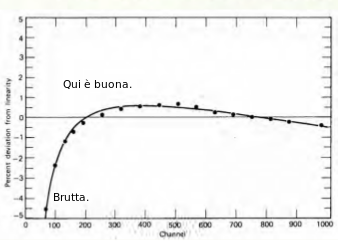
\includegraphics[scale=1.00]{./Immagini/LinearitaScintillatore.png}
\caption{Percentuale di deviazione dalla linearit\`a per uno scintillatore. Esiste un range dove essa \`e rispettata.}
\end{center}
\end{figure}
\subsection{Calibrazione in energia dei rivelatori}
Per calibrare i rivelatori si usano delle sorgenti ad energie note, in generale si cerca di usare dei $\gamma$ con energie ben spaziate
su tutto il range energetico di interesse.
I raggi $\gamma$ sono noti con una precisione energetica di $10^{-5}$, per questo \`e importante utilizzare sorgenti note con quella
precisione, per questo motivo esistono delle sorgenti standard di calibrazione:
\begin{itemize}
\item K$_{\alpha}$(W) (tungsteno) a 5.9 keV
\item $^{198}$Au a 412 keV
\item $^{60}$Co a 1333 keV
\end{itemize}
\textbf{Non si possono usare i fotoni di annichilazione} in quanto il decadimento non avviene sempre a riposo.\\
Inoltre se ho una fuga singola o doppia in una regione ben calibrata, posso usarla per controllare la correttezza della calibrazione,
lo stesso vale nel caso dell'emissione in cascata di fotoni.\\
La curva di calibrazione viene ottenuta interpolando i punti con una funzione polinomiale del tipo
\begin{equation*}
E_i = \sum_{n=0}^N a_n C_i^n
\end{equation*}
con $N \approx 4-5$ utilizzando il metodo dei minimi quadrati.\\
Sono state osservate dipendenze dalla direzione di incidenza della radiazione della risposta, per questo motivo \`e necessario calibrare
tenendo conto del lato che verr\`a esposto alla radiazione. 
Queste variazioni sono nell'ordine dei 100 eV, per questo motivo diventano importanti per misure molto precise;
questo accade perch\`e il campo elettrico degli elettroni influisce sulla raccolta dei fotoni.
\subsection{Convenzioni sulle efficienze nella spettroscopia $\gamma$}
Alcuni rapporti sono molto diffusi nella descrizione delle efficienze dei rivelatori:
\begin{itemize}
\item \textbf{Rapporto picco-Compton}, viene definita sul decadimento del $^{137}$Cs  a 662 keV come:
\begin{equation*}
R_{pc} = \frac{\text{Conteggi/canale al canale del massimo}}{\text{Conteggi/canale medi nella regione tra 358 e 382 keV}}
\end{equation*}
oppure sul decadimento del $^{60}$Co a 1333 keV:
\begin{equation*}
R_{pc} = \frac{\text{Conteggi/canale al canale del massimo}}{\text{Conteggi/canale medi nella regione tra 1040 e 1096 keV}}
\end{equation*}
Gli intervalli di energia sono stati scelti in quanto in quella regione non \`e presente radiazione naturale, ma solamente Compton.
Questo parametro serve a dare una misura combinata della FWHM con la fotofrazione $R_{ph}$:
\begin{equation*}
R_{ph} = \frac{\text{Area del picco ad energia piena}}{\text{Area totale dello spettro}}
\end{equation*}
$R_{pc}$ viene peggiorato dallo scattering Compton con l'ambiente.
A parit\`a di fotofrazione si osserva che $R_{pc} \propto \frac{1}{\text{FWHM}}$ e, a parit\`a di FWHM, $R_{pc} \propto R_{ph}$ (\textbf{perch\`e?}).
\item \textbf{Efficienza assoluta del picco ad energia piena} $\epsilon_{ap}$
\item \textbf{Efficienza intrinseca del picco ad energia piena} $\epsilon_{ip}$, tipicamente viene quotato per $^60$Co a 1333 keV
\item \textbf{Volume attivo}, ad alte energie $\epsilon_{ip} \propto V_{att}$
\item \textbf{Efficienza relativa}, a volte l'efficienza viene quotata rispetto all'efficienza di un rivelatore a NaI di $3''\times 3''$ 
con sorgente di $^{60}$Co posta a 25 cm di distanza con fotoni a 1333 keV, questa efficienza vale $\epsilon_{ap} = 1.2 \cdot 10^{-3}$
\item \textbf{Regola del pollice}, poich\`e l'efficienza ha una dipendenza dal volume, a volte viene data per unit\`a di volume, ad esempio per il germanio (rivelatore HPGe) vale:
\begin{equation*}
\epsilon_{rel}^{Ge} \approx \frac{V[\text{cm}^3]}{5}\%
\end{equation*}
Per cui un germanio al 100\% ha un volume di 500 cm$^3$.
\end{itemize}
\chapter{Rivelatori a gas}
\section{Principio di funzionamento}
In un rivelatore a gas \`e formato da una camera piena di materiale gassoso posto tra due elettrodi a diverso potenziale:
quando una particella carica (ionizzante) incide sulla camera, libera coppie di elettroni e ioni; 
queste cariche migrano verso gli elettrodi stabilendo una corrente che \`e proporzionale all'energia deposta nella camera.
Se supponiamo di avere liberato $N$ coppie in seguito alla deposizione di un'energia $E$, allora si pu\`o definire:
\begin{equation*}
W = \frac{E}{N}
\end{equation*}
ovvero l'energia media necessaria per liberare una coppia elettrone-ione.
Questa quantit\`a \`e in genere maggiore dell'energia di legame degli elettroni periferici (25-35 eV), in quanto tiene conto di quell'energia che
viene spesa in eccitazioni atomiche senza ionizzazione.
Gli elettroni prodotti in seguito ad un evento sono in grado di produrre ulteriore ionizzazione, chiamata ionizzazione secondaria, che verr\`a, in
ultima analisi, considerata.\\
Il parametro $W$ \`e un parametro con una blanda dipendenza da tipo di particella e dall'energia deposta,
mentre ha una dipendenza un po' pi\`u pronunciata dal tipo di gas (fig.~\ref{fig:energiaIonizzazioneGas}).
\begin{figure}[htbp]
\begin{center}
	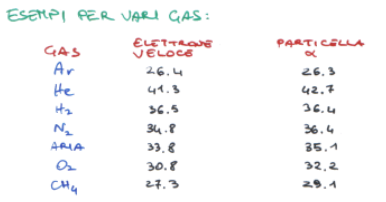
\includegraphics[scale=1]{./Immagini/EnergiaIonizzazioneGas.png}
\caption{Energia di ionizzazione per alcuni gas}
\label{fig:energiaIonizzazioneGas}
\end{center}
\end{figure}
Le fluttuazioni sul numero di coppie prodotte sono di tipo poissoniano:
\begin{equation*}
\sigma_N^2 =F \cdot N
\end{equation*}
con $F$ fattore di Fano, esso \`e minore di 1 nei gas.
\section{Processi all'interno di un rivelatore a gas}
\subsection{Diffusione}
Gli ioni e gli elettroni prodotti all'interno di un gas si diffondono per moto termico; il tipico libero cammino medio per uno ione \`e dai 
$10^{-6}$ ai $10^{-8}$ m.
La diffusione termica degli elettroni \`e di tipo gaussiano con una larghezza che dipende dal tempo secondo la legge:
\begin{equation*}
\sigma = \sqrt{2D\, t}
\end{equation*}
Il coefficiente $D$ di diffusione pu\`o essere determinato nei casi semplici dalla teoria cinetica dei gas, altrimenti tramite modelli di trasporto complessi.
\subsection{Il trasferimento di carica}
Supponiamo di avere due specie X e Y di gas miscelate, quando produco ionizzazione su X posso dar luogo ad una serie di processi detti di trasferimento di carica:
\begin{itemize}
\item L'elettrone che viene liberato viene catturato da Y, di conseguenza ho una coppia (X$^+$, Y$^{-}$)
\item L'atomo ionizzato X$^+$ sottrae carica a un atomo non ionizzato Y, di conseguenza ho una coppia (Y$^{-}$, e$^-$)
\end{itemize}
\subsection{Ricombinazione}
\`E il processo per cui due specie ionizzate X$^-$ e Y$^+$ si neutralizzano formando una specie XY.
Vale la relazione:
\begin{equation*}
\frac{dn^+}{dt} = \frac{dn^-}{dt} = - \alpha \, n^+ \, n^-
\end{equation*}
con $\alpha$ coefficiente di ricombinazione.\\
Esistono due tipi di ricombinazione:
\begin{itemize}
\item \textbf{Ricombinazione colonnare}, avviene immediatamente lungo la traccia della particella ed \`e fortemente dipendente dalla densit\`a di ionizzazione prodotta dalla particella.
Ad esempio le particelle $\alpha$ potranno dar luogo ad un elevata ricombinazione colonnare.
\item \textbf{Ricombinazione volumetrica}, avviene in un secondo momento lontano dalla traccia della particella per la propagazione
delle cariche pi\`u mobili come gli elettroni. Avvenendo dopo un certo tasso di tempo e lontano dalla traccia, la ricombinazione pu\`o avvenire tra ionizzazioni
dovute a tracce differenti, per cui \`e fortemente dipendente dal rate di particelle
\end{itemize}
Per contrastare la ricombinazione volumetrica \`e importante sottoporre il volume ad una differenza di potenziale elevata, in modo da estrarre 
rapidamente ed efficacemente le cariche.
\section{La mobilit\`a e la migrazione delle cariche}
Supponiamo di sottoporre le cariche ad un campo elettrico \textbf{E}, esse migreranno a seconda della carica verso i rispettivi elettrodi.
In generale le collisioni faranno si che esister\`a una velocit\`a media, detta \textbf{velocit\`a di deriva}, tale velocit\`a dipende dal campo
elettrico e dalla pressione secondo la relazione:
\begin{equation*}
v = \mu \frac{\mathbf{E}}{p}
\end{equation*}
con $\mu$ coefficiente di mobilit\`a delle cariche.
Questo coefficiente per gli ioni vale nei $10^{-4}$, portando ad avere diffusioni lente;
per gli elettroni \`e 1000 volte pi\`u  grande (massa 1000 volte pi\`u piccola) portando i tempi per raggiungere gli elettrodi nei $\mu$s.
Il coefficiente \`e costante in ampii range di pressione e campo elettrico per gli ioni, mentre per gli elettroni lo \`e solo per un 
range ristretto di pressione e campo, per via della saturazione.\\
Un'ultima osservazione va fatta per quanto riguarda la diffusione termica: campi pi\`u intensi porteranno ad avere energie e diffusioni maggiori negli elettroni,
per cui si avr\`a una maggiore diffusione in direzione perpendicolare.
Questo non \`e un problema per la raccolta delle cariche, tuttavia disperde gli elettroni (nel mm), facendo perdere risoluzione spaziale.
\section{Le camere a ionizzazione}
\begin{figure}[htbp]
\begin{center}
	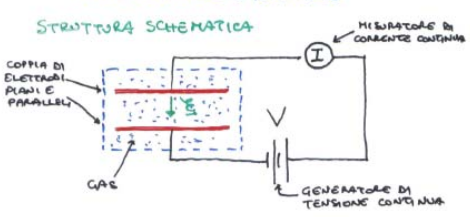
\includegraphics[scale=1]{./Immagini/CameraIonizzazione.png}
\caption{Struttura schematica di una camera a ionizzazione}
\label{fig:cameraIonizzazione}
\end{center}
\end{figure}
\`E un rivelatore che funziona in modalit\`a integrata, in quanto permette di misurare il flusso di radiazione ionizzante.
Supponiamo di avere un flusso di radiazione incidente, esso potr\`a dare luogo ai tre fenomeni: ricombinazione, diffusione fuori dalla camera o verso gli elettrodi;
l'ultimo tipo di evento \`e quello che produce una misura, per contrastare gli altri due \`e necessario aumentare la tensione ai capi della camera.
All'aumentare della tensione si osserva, infatti, un aumento della corrente, fino al raggiungimento di un plateau (fig.~\ref{fig:saturazione}) dovuto alla raccolta completa delle cariche,
in queste condizioni di parla di saturazione del rivelatore e sono le condizioni ottimali di lavoro.
\begin{figure}[htbp]
\begin{center}
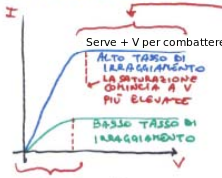
\includegraphics[scale=1]{./Immagini/Saturazione.png}
\caption{Curva tensione-corrente in una camera a ionizzazione, si nota la saturazione}
\label{fig:saturazione}
\end{center}
\end{figure}
Vediamo i fattori che influiscono sulla corrente di saturazione.\\
Il \textbf{tipo di particella} \`e importante, particelle cariche pesanti causano una maggiore ricombinazione colonnare, per cui portano pi\`u in alto il valore
minimo della tensione di saturazione.\\
Un maggiore \textbf{tasso di irraggiamento} implica una maggiore ricombinazione volumetrica, portando in alto la tensione minima.\\
Nel caso vengano usate camere ad aria,\textbf{ l'umidit\`a }\`e un fattore che influisce sulla ricombinazione volumetrica, aumentandola, per questo maggiori umidit\`a
alzano la tensione minima.\\
A causa del moto di deriva delle cariche, lungo gli elettrodi si forma un accumulo di carica che tende a schermarli e a rendere pi\`u difficile la raccolta delle cariche.
Si pu\`o immaginare che si formi un potenziale opposto che genera una corrente di contrasto, \`e possibile trovare la variazione relativa attraverso:
\begin{equation*}
\frac{\Delta I}{I} = \epsilon \frac{k_b T}{e\cdot V}
\end{equation*}
con T temperatura ed $\epsilon$ il rapporto tra l'energia media della particella sotto l'effetto del campo elettrico ed in sua assenza.
Questo rapporto vale circa 1 per gli ioni, ma vale alcune centinaia per gli elettroni.
Per gli elettroni l'energia media raggiunge un plateau all'aumentare della tensione, per questo motivo \`e possibile contrastare questa variazione
di corrente opponendo campi elettrici pi\`u intensi, quindi tensioni maggiori.\\
Per tensioni sufficientemente alte, la ricombinazione volumetrica pu\`o diventare trascurabile, tuttavia questo non accade per la colonnare;
per questo motivo la corrente misurata sar\`a sempre minore della corrente reale di saturazione.
Una stima di quanta corrente si sta perdendo pu\`o essere ottenuto costruendo una curva 1/V - 1/I, interpolandola ed estrapolando il punto a 1/V = 0, ovvero
V infinita (fig~\ref{fig:iPersa}).
\begin{figure}[htbp]
\begin{center}
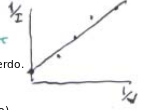
\includegraphics[scale=1]{./Immagini/IPersa.png}
\caption{Stima della corrente di saturazione}
\label{fig:iPersa}
\end{center}
\end{figure}
\section{Funzionamento in modo impulsivo delle camere a ionizzazione}
Il moto delle cariche all'interno della camera induce una corrente ai capi degli elettrodi, questa variazione viene percepita
da un sistema RC che raggiunge una tensione massima quando tutta la carica viene raccolta.
Il tempo caratteristico del circuito determina il tipo di carica raccolta: RC nei $\mu$s saranno sensibili solamente alla raccolta degli elettroni,
RC nei ms saranno sensibili anche alle particelle cariche.
Chiaramente la scelta di RC determina il tasso che il rivelatore \`e in grado di misurare, un RC nei $mu$s sar\`a in grado di rivelare e misurare
a tassi maggiori, tuttavia produrr\`a segnali pi\`u piccoli.
\subsection{Sviluppo del segnale nel tempo}
\begin{figure}[htbp]
\begin{center}
	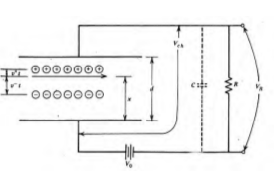
\includegraphics[scale=1]{./Immagini/CircuitoCameraIonizzazione.png}
\end{center}
\end{figure}
Per ottenere lo sviluppo del segnale nel tempo ricorriamo alla conservazione dell'energia, ponendo $V_0$ la tensione iniziale e $V_{ch}$ quella rimanente si ha:
\begin{equation*}
\frac{1}{2} C V_0^2 = n_0 e E v^+ t - n_0 e E v^- t + \frac{1}{2}C V_{ch}^2
\end{equation*}
Portando a sinistra i termini legati al condensatore e dato che $E=-V_{ch}/d$ con $d$ distanza tra gli elettrodi su pu\`o scrivere:
\begin{equation*}
\frac{1}{2} C (V_0+V_{ch})(V_0-V_{ch}) = n_0 e \left(\frac{V_{ch}}{d}\right) t (v^+ - v^-)
\end{equation*}
Dato che $V_{ch}\approx V_0$, $V_0+V_{ch}\approx 2 V_0$ e $V_0 - V_{ch} = V_R$, ovvero la tensione sulla resistenza possiamo scrivere:
\begin{equation}\label{eq:VRCamera}
V_R = \frac{n_0 e (v^+-v^-)}{d\,C}t
\end{equation}
Da cui si pu\`o vedere che la porzione iniziale del segnale ha andamento lineare dipendente dal numero di coppie liberate.
Dalla relazione~\ref{eq:VRCamera} si possono osservare alcune cose:
\begin{itemize}
\item Il moto delle cariche positive ha indotto un potenziale $\frac{n_0 e v^+}{d\,C}t$, lo stesso vale per le negative. 
Questo potenziale pu\`o essere visto come una carica indotta $\frac{n_0 e v^+}{d}t$ ai capi della capacit\`a.
\item Quando la raccolta delle cariche si \`e conclusa $v^- t$ vale $-x$ (\`e opposto al campo) e $v^+ t$ vale $d-x$, per cui si ha:
\begin{equation*}
V_R^{MAX} = \frac{n_0 e}{C}
\end{equation*}
\end{itemize}
\section{Le camere proporzionali}
Supponiamo che una particella da 1 MeV ionizzi il gas contenuto in una camera a ionizzazione, se l'energia media di ionizzazione \`e 35 eV e il condensatore
ha una capacit\`a di 100 pF allora l'ampiezza massima del segnale generato sar\`a:
\begin{equation*}
V_{MAX} = \frac{E\,e}{W \, C} \sim 10 \mu\,\text{V}
\end{equation*}
Il segnale \`e piuttosto piccolo, per questo motivo \`e necessario amplificando cercando di utilizzare la ionizzazione secondaria:
le camere proporzionali si basano su questo principio, le cariche primarie liberate vengono accelerate da un campo che fornisce loro energia sufficiente
a produrre ionizzazione a cascata, come in una sorta di fotomoltiplicatore.
La quantit\`a di ionizzazione prodotta risulta dipendente dalla ionizzazione primaria, quindi dall'energia iniziale della particella, e il segnale
molto pi\`u forte rispetto a quelle prodotto da un rivelatore basato unicamente sulla ionizzazione primaria.\\
Una geometria molto utilizzata in questi rivelatori \`e quella cilindrica: in questi rivelatori il campo elettrico scala come il reciproco del raggio;
per l'aria, se esso supera il valore soglia di $10^6$ V/m allora si possono osservare moltiplicazioni di ionizzazione.
Per un rivelatore dove il campo \`e costante la moltiplicazione \`e esponenziale:
\begin{equation*}
n(x) = n(0) e^{\alpha x}
\end{equation*}
con $x$ spazio percorso e $\alpha$ coefficiente di Townsend.
Questo coefficiente dipende dal campo con l'andamento riportato in figura~\ref{fig:townsend}, per cui per un rivelatore a geometria cilindrica
la moltiplicazione \`e pi\`u che esponenziale.
\begin{figure}[htbp]
\begin{center}
	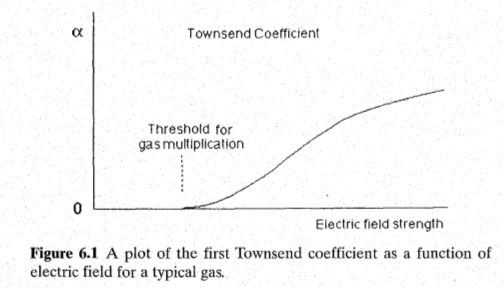
\includegraphics[scale=0.8]{./Immagini/Townsend.png}
\caption{Coefficiente di Townsend}
\label{fig:townsend}
\end{center}
\end{figure}
\subsection{Problemi delle camere proporzionali}
Uno dei problemi fondamentali nelle camere proporzionali sta nella scelta del gas: poich\`e gli elettroni possono ionizzare, eccitare o essere assorbiti a seconda
della molecola con cui interagiscono, la composizione del gas \`e fondamentale.
Ad esempio un gas elettronegativo come l'ossigeno pu\`o essere un problema, per via della sua tendenza ad attrarre elettroni; la presenza di molecole
pu\`o portare ad eccitazioni e diseccitazioni non radiative (mediante stati vibrazionali eccitati).\\
In genere vengono usati gas nobili, come l'Argon, che dissipano l'energia principalmente per ionizzazione; questi, tuttavia, hanno il problema
della diseccitazione, poich\`e essa pu\`o passare unicamente attraverso emissione di fotoni (non ho molecole che si eccitano vibrazionalmente) questi possono
ionizzare gli elettrodi, generando ulteriori scariche a valanga.
Queste scariche possono allungare la durata degli impulsi e il tempo morto del dispositivo, per questo spesso si accompagna questi gas con dei gas
quenchanti che spengono la valanga eccitandosi vibrazionalmente.
Un esempio di gas quenchante \`e il metano che assorbe nella fascia dei 10 eV.
\section{Fluttuazioni statistiche nelle camere proporzionali}
Nelle camere proporzionali abbiamo due principali cause di fluttuazioni statistiche:
\begin{itemize}
\item Fluttuazione nel numero di elettroni primari liberati
\item Fluttuazione nella moltiplicazione del singolo elettrone primario
\end{itemize}
Se supponiamo che le due fluttuazioni siano indipendenti, allora \`e possibile trovare la fluttuazione relativa complessiva sommando gli errori relativi in quadratura;
ponendo $\bar{A}$ la media dei fattori di moltiplicazione di un singolo elettrone si pu\`o scrivere:
\begin{equation*}
\left(\frac{\sigma_{Q}}{Q}\right)^2 = \left(\frac{\sigma_{n_0}}{n_0}\right)^2 +  \left(\frac{\sigma_{\bar{A}}}{\bar{A}}\right)^2
\end{equation*}
La varianza del fattore medio di moltiplicazione vale:
\begin{equation*}
\sigma^2_{\bar{A}} = \frac{\sum_i^{n_0} \sigma^2_A}{n_0^2} = \frac{\sigma^2_A}{n_0}
\end{equation*}
con $\sigma_A$ varianza del fattore di moltiplicazione di singolo elettrone.
Si pu\`o quindi scrivere
\begin{equation*}
\left(\frac{\sigma_{Q}}{Q}\right)^2 = \left(\frac{\sigma_{n_0}}{n_0}\right)^2 + \frac{1}{n_0} \left(\frac{\sigma_{A}}{\bar{A}}\right)^2
\end{equation*}
Il primo termine \`e gi\`a stato trattato nelle camere a ionizzazione, esso vale:
\begin{equation*}
\left(\frac{\sigma_{n_0}}{n_0}\right)^2 = \frac{F}{n_0}
\end{equation*}
Per quanto riguarda il secondo termine, nel caso di bassi campi elettrici \`e possibile ipotizzare che la probabilit\`a di ionizzazione di un elettrone non dipenda dalla sua storia;
se $A>100$ \`e possibile scrivere la probabilit\`a di avere un determinato $A$ al termine di un amplificazione come:
\begin{equation*}
P(A) = \frac{e^{-A}{\bar{A}}}{\bar{A}}
\end{equation*} 
per cui:
\begin{equation*}
\left(\frac{\sigma{A}}{A}\right)^2 = 1
\end{equation*}
Se il campo \`e intenso l'ipotesi di indipendenza dalla storia salta ed \`e necessario considerare un modello pi\`u complesso che porta ad affermare:
\begin{equation*}
\left(\frac{\sigma_A}{A}\right)^2 = \frac{1}{\bar{A}} + b
\end{equation*}
con $b = (1+\theta^2)^{-1}\approx 0.5$ e $\theta$ \`e un parametro che dipende dalla frazione di elettroni con energia superiore a quella di ionizzazione.
\subsection{Sviluppo del segnale}
In una camera proporzionale esistono due tempi caratteristici: il tempo di deriva, che indica il tempo impiegato dagli elettroni a raggiungere la zona
di moltiplicazione (ovvero la regione prossima all'anodo), e il tempo di moltiplicazione, ovvero il tempo impiegato dagli elettroni per effettuare la loro moltiplicazione a cascata.
Il moto delle coppie primarie \`e trascurabile ai fini della forma del segnale, in quanto producono segnali molto piccoli, per questo si pu\`o
dire che i segnali prodotti dalla camera hanno un ritardo nell'ordine del $\mu$s rispetto all'evento, per via del drift delle cariche.
Il tempo di moltiplicazione \`e molto inferiore rispetto a quello di deriva, per cui il tempo di ritardo pu\`o essere assunto pari al tempo di drift.\\
Dato che il segnale viene prodotto vicino all'anodo, il fronte di salita del segnale viene determinato sopratutto dal moto degli ioni positivi:
essi sono immersi in campi intensi che li portano ad avere un'alta velocit\`a di deriva verso il catodo.
Per questo motivo il fronte di salita \`e inizialmente molto veloce, successivamente diventa lento, in quanto gli ioni entrano nella zona a campo debole in cui
sono lenti.\\
Mostriamo che il segnale \`e fortemente dipendente dal moto degli ioni, chiamiamo $E$ l'energia e $\epsilon$ il campo, iniziamo
con il calcolare tempo necessario affinche uno ione raggiunga il catodo.
Si pu\`o approssimare che gli ioni vengano prodotti a ridosso dell'anodo, quindi a raggio $a$, la velocit\`a dello ione vale:
\begin{equation*}
v^+ = \mu \frac{\epsilon}{p} = \frac{\mu}{p} \frac{V_0}{r \, \text{ln}(b/a)}
\end{equation*}
Risolvendo l'equazione differenziale per separazione delle variabili:
\begin{equation*}
v^+(r) = \frac{dr}{dt}
\end{equation*}
si ottiene:
\begin{equation*}
r(t) = \sqrt{2 \frac{\mu}{p} \frac{V_0}{\text{ln}(b/a)} t + a^2}
\end{equation*}
per cui il tempo per raggiungere $b$ vale:
\begin{equation*}
t^+ =\frac{(b^2 - a^2) p \, \text{ln}(b/a)}{2 \mu V_0}
\end{equation*}
Inserendo dati tipici si ottiene che questo tempo vale nelle centinaia di $\mu$s;
studiando l'andamento temporale dell'energia si ottiene, tuttavia, che la maggior parte del segnale si sviluppa in breve tempo:
\begin{equation*}
\frac{1}{2} C \, V_0^2 - \frac{1}{2} C \, V_{ch}^2 = \Delta E
\end{equation*}
in modo simile a quanto fatto prima, si trova che $V_R = V_0 - V_{ch}$ vale:
\begin{equation*}
V_R(t) = \frac{\Delta E(t)}{C V_0}
\end{equation*}
Calcoliamo $\Delta E(t)$:
\begin{equation*}
\frac{dE}{dx} = Q \epsilon = Q \frac{V_0}{r \, \text{ln}(b/a)}
\end{equation*}
per cui:
\begin{equation*}
\Delta E(t) = \frac{Q \, V_0}{ \, \text{ln}(b/a)} \int_a^{r(t)} \frac{1}{r} \, dr  =  \frac{Q \,V_0}{ \text{ln}(b/a)} \text{ln}\left(\frac{r(t)}{a}\right)
\end{equation*}
Usando $r(t)$ trovato predecentemente si trova:
\begin{equation*}
V_R(t) =\frac{ \Delta E(t)}{C \, V_0} = \frac{Q}{C} \frac{1}{\text{ln}(b/a)} \text{ln} \left(\frac{2\mu V_0}{a^2 p \text{ln}(b/a)}t+1\right)^{\frac{1}{2}}
\end{equation*}
Il tempo affinche si raggiunga mezza ampiezza vale:
\begin{equation*}
t = \frac{a}{a+b} t^+
\end{equation*}
ed \`e nei $\mu$s.\\
Questi conti sono validi nell'ipotesi di elettroni moltiplicati in un punto fisso, altrimenti si osserva uno spreading dei tempi.\\
Tipicamente i tempi del RC non sono tali da permettere una raccolta completa delle cariche, per questo si ha il problema del deficit balistico.
Infine gli elettroni contribuiscono nel \% all'ampiezza del segnale, in quanto percorrono poco spazio nella camera.
\section{Contatori Geiger-M\"uller}
\begin{figure}[htbp]
\begin{center}
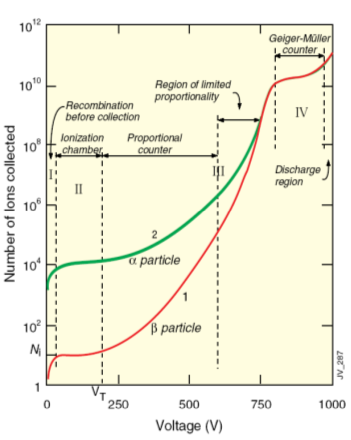
\includegraphics[scale=1]{./Immagini/RegioniGas.png}
\caption{Regioni di lavoro di un rivelatore a gas}
\label{fig:regioniGas}
\end{center}
\end{figure}
Aumentando la tensione ai capi di una camera a gas si pu\`o aumentare ulteriormente la moltiplicazione degli elettroni, in particolare si pu\`o raggiungere
una regione detta di saturazione, dove si satura la camera e ogni evento produce la medesima ionizzazione.
Questa regione \`e quella in cui operano i rivelatori di Geiger-M\"uller: questi dispositivi producono impulsi medesimi indipendentemente dalla ionizzazione
iniziale (quindi dall'energia).
Questi rivelatori non sono, quindi, adatti per misure di spettroscopia, tuttavia possono essere utilizzati come contatori a bassi rate.
L'elevato fattore moltiplicativo dei contatori Geiger ($\sim 10^{10}$) produce segnali nei volt che possono essere usati per alimentare un altoparlante, da qui
il click tipico di questi dispositivi.
La cascata in questi dispositivi \`e fortemente determinata dalla diseccitazioni dei gas, infatti esse producono fotoni nell'ultravioletto in grado
di produrre scariche secondarie in regioni remote del gas (dato che ha bassa probabilit\`a di assorbire il fotone) generando ulteriori
valanghe e fotoni UV (fig.~\ref{fig:valangaGM}).
Per questo motivo nei GM non \`e possibile determinare il punto di interazione della particella incidente.
\begin{figure}[htbp]
\begin{center}
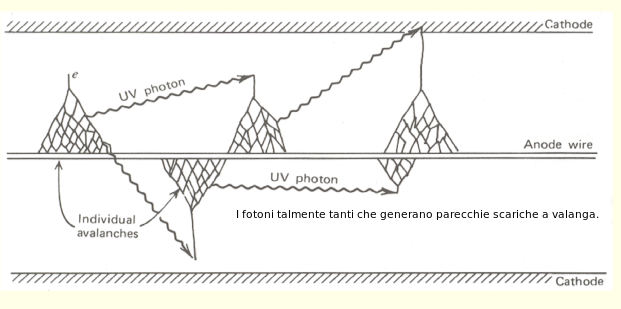
\includegraphics[scale=0.7]{./Immagini/ValangaGM.png}
\caption{Scarica in un contatore GM}
\label{fig:valangaGM}
\end{center}
\end{figure}
Il gas usato nei rivelatori \`e spesso un gas nobile, ma \`e possibile utilizzare anche l'aria.\\
La scarica prodotta nei GM \`e talmente violenta che \`e necessario introdurre dei meccanismi di spegnimento della moltiplicazione,
spesso si procede con un interruzione dell'alimentazione dopo un certo tempo. 
Questa interruzione porta ad avere tempi morti piuttosto elevati, per questo i GM non possono essere utilizzati in caso di alti rate di interazione.\\
Per quanto concerne i segnali, i fronti di salita dei GM sono pi\`u lenti di quelli delle camere proporzionali, per via delle valanghe lontane,
in genere sono nei $\mu$s. 
I fronti di discesa sono molto pi\`u lenti, si usano formature con tempi inferiori a 100 $\mu$s.
Il tempo morto in questi dispositivi \`e nei 100 $\mu$s, in quanto \`e necessario assicurarsi che non siano presenti ulteriori scariche libere
che possano generare scariche all'accensione del campo elettrico.
Inoltre le cariche positive libere riducono il campo elettrico, impedendo la formazione di nuove cascate, influendo sul tempo morto.
\chapter{Rivelatori a semiconduttore}
L'utilizzo di camere a ionizzazione a stato solido con semiconduttori pu\`o semplificare notevolmente la struttura di un rivelatore:
l'elevata densit\`a di portatori di carica permette, infatti, di ottenere rivelatori di dimensioni ridotte (sono sufficienti 300 $\mu$m di Si), inoltre,
grazie alla bassa energia di ionizzazione e alla presenza di portatori di carica positivi e negativi, \`e possibile ottenere segnali sufficientemente
ampii senza ricorrere alla moltiplicazione.
Per utilizzare questi rivelatori \`e necessario che le cariche abbiano una vita media elevata e che la loro mobilit\`a sia sufficiente, pur mantenendo
una corrente di buio ridotta.
Queste caratteristiche sono presenti nel silicio, germanio e GaAs, sebbene i primi due a temperatura ambiente abbiano una corrente di buio troppo elevata.
\section{Semiconduttori intrinseci}
In un semiconduttore intrinseco il numero di portatori di carica in banda di conduzione pu\`o essere determinato attraverso:
\begin{equation*}
n^2 = N_c N_v e^{\frac{E_g}{k_B T}}
\end{equation*}
con $N_c$ numero di stati ai margini della banda di conduzione e $N_v$ in banda di valenza.
Posto $n$ il numero di portatori di carica negativi e $p$ numero di quelli positivi (lacune) vale
che $n=p$ e che $np=n^2$.
In un silicio a temperatura ambiente $n_i \sim 10^{10}$ e in un germanio $\sim 10^{13}$.\\
Per quanto riguarda la resistivit\`a di questi materiali, la velocit\`a delle cariche \`e data dalla relazione:
\begin{equation*}
v = \mu_{e,h} \, E
\end{equation*}
La mobilit\`a delle lacune \`e inferiore, ma dello stesso ordine di grandezza, rispetto a quella degli elettroni;
in generale la resistivit\`a pu\`o essere definita come:
\begin{equation*}
\rho = \frac{1}{q(\mu_n n + \mu_h p)}
\end{equation*}
Nel Si o Ge intrinseco, il numero di portatori di carica liberi per agitazione termica \`e troppo pi\`u grande rispetto a quelli prodotti
dalla ionizzazione, per questo non sono utilizzabili nella forma pura ed \`e necessario ricorrere alle giunzioni di materiali drogati.
\section{Semiconduttori estrinseci o drogati}
Introducendo delle impurezze nel cristallo semiconduttore si effettua l'operazione di drogaggio; mediante il drogaggio del materiale si riescono ad ottenere conducibilit\`a maggiori.
Esistono due tipi di drogaggio:
\begin{itemize}
\item tipo p, si introduce un materiale con un elettrone di valenza in meno e si introduce uno stato intermedio spostato verso la banda di valenza;
in questo modo si favorisce la presenza di lacune nel materiale
\item tipo n, si introduce un materiale con un elettrone di valenza in pi\`u e si introduce uno stato intermedio spostato verso la banda di conduzione;
in questo modo si favorisce l'elettrone eccedente ad entrare nella banda di conduzione
\end{itemize}
Introducendo le impurezze, le energie di ionizzazione vanno nei meV, rendendo il materiale un buon conduttore a temperatura ambiente.\
Chiamando $N_D$ il numero di donori (impurezze tipo n) e $N_A$ il numero di accettori (tipo p) se esse sono numerose si pu\`o affermare
che $n \approx N_D$ (in un tipo n) oppure $p \approx N_A$ (in un tipo p).
Inoltre il numero di portatori di carica di segno opposto potr\`a essere calcolato come:
\begin{equation*}
p \;(n) = \frac{n_i^2}{n \; (p)} \approx \frac{n_i^2}{N_D\;(N_A)}
\end{equation*}
In queste condizioni di drogaggio si parla di \textbf{semiconduttori estrinseci};
se $N_A \asymp N_D$ si parla di materiali compensati, se $N_{A,D} \ge 10^{19} - 10^{20}$ cm$^{-3}$ si parla di materiali pesantemente drogati
in quanto si \`e raggiunto il livello di conducibilit\`a dei metalli.
\section{Rivelatori basati su i semiconduttori}
\`E possibile immaginare un rivelatore che si occupi di raccogliere le coppie elettrone-lacuna prodotte in un cristallo semiconduttore in seguito
alla ionizzazione prodotta da una particella.
In un semiconduttore l'energia media per produrre una coppia lacuna-elettrone \`e nell'ordine dei 3 eV (simile al gap di energia tra le bande),
circa 10 volte inferiore a quello nei gas: questo si ripercuote sulla risoluzione, che migliora notevolmente.
Una stima brutale del miglioramento pu\`o essere fatta in approssimazione di risoluzione poissoniana:
poich\`e, a parit\`a di energia, in un semiconduttore si producono 10 volte pi\`u cariche rispetto ad un gas, allora il rapporto tra le risoluzioni
percentuali ($\propto \frac{1}{\sqrt{N}}$) vale:
\begin{equation*}
\frac{R_{SEMI}}{R_{GAS}} = \frac{\sqrt{N}}{\sqrt{10 N}} \approx \frac{1}{3}
\end{equation*}
per cui la risoluzione migliora di un fattore $\frac{1}{3}$. 
In realt\`a, il miglioramento \`e ancora maggiore per via del fattore di Fano.\\
La configurazione pi\`u semplice attuabile porterebbe a introdurre del silicio puro tra due elettrodi, ma purtroppo l'elevata conducibilit\`a
del silicio porta ad avere correnti di buio troppo grandi rispetto alle correnti prodotte dagli eventi;
per questo motivo \`e necessario ricorrere alle giunzioni tra materiali drogati.
\section{La giunzione p-n}
Consideriamo due semiconduttori drogati uno di tipo p e uno di tipo n.
Da un lato si ha una sovrabbondanza di lacune, dall'altra una sovrabbondanza di elettroni;
quando i due semiconduttori vengono messi a contatto, si forma una corrente detta di diffusione dovuta alla ricombinazione delle lacune con gli elettroni.
Lungo la giunzione si forma un accumulo di carica: lungo il lato p gli elettroni giunti a compensarsi con le lacune causano un accumulo di carica
negativa, dall'altro lato rimane un accumulo di carica positiva.
A questo punto si instaura una seconda corrente, legata alla differenza di potenziale associata alla distribuzione di carica, questa corrente
si compensa con quella di diffusione (sono opposte) dando vita alla situazione di equilibrio.
All'equilibrio (figura~\ref{fig:equilibrioPN}) sono presenti 3 regioni, una di tipo p, una di tipo n ed in mezzo una regione dove sono unicamente presenti i portatori di carica intrinseci.
Quest'ultima regione viene detta di svuotamento.
\begin{figure}[htbp]
\begin{center}
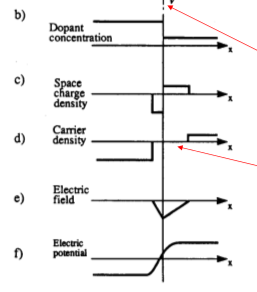
\includegraphics[scale=1]{./Immagini/EquilibrioPN.png}
\caption{Condizione di equilibrio in una giunzione PN}
\label{fig:equilibrioPN}
\end{center}
\end{figure}
Quando viene applicata una differenza di potenziale concorde con quella della regione di svuotamento, la regione si allarga, la corrente di diffusione
diminuisce, mentre quella di generazione (dovuta alla differenza di potenziale alla giunzione) rimane costante.
Come risultato si ottiene un'aumento della corrente di fuga $\propto e^{\frac{qV}{k_B T}}$.
\subsection{Dimensioni della regione di svuotamento}
Supponiamo di aver usato materiali drogati n e p in modo diverso, all'equilibrio la dimensione della regione di svuotamento nelle zone sar\`a asimmetrica.
Se poniamo $N_A$ e $N_D$ la densit\`a lineare di accettori e donori, all'equilibrio vale:
\begin{equation}\label{eq:consCaricaSemicond}
N_A \cdot a = N_D \cdot b
\end{equation}
La densit\`a di carica lineare sar\`a:
\begin{equation*}
\rho (x) = 
\begin{cases}
-e N_A \; \; $se $-a<x<0\\
e N_D \; \; $se $0<x<b
\end{cases}
\end{equation*}
L'equazione di Poisson afferma:
\begin{equation*}
\frac{d^2 \varphi}{dx^2} = \frac{-\rho(x)}{\varepsilon}
\end{equation*}
Integrando una volta la distribuzione di carica si pu\`o ottenere l'opposto del campo elettrico:
\begin{equation*}
-E (x) = 
\begin{cases}
-\frac{e N_A x}{\varepsilon} + c_1 \; \; $se $-a<x<0\\
\frac{e N_D x}{\varepsilon} + c_2 \; \; $se $0<x<b
\end{cases}
\end{equation*}
Imponendo le condizioni al contorno $E(-a)=E(b)=0$ si ottiene:
\begin{equation*}
-E (x) = 
\begin{cases}
-\frac{e N_A (x+a)}{\varepsilon}  \; \; $se $-a<x<0\\
\frac{e N_D (x-b)}{\varepsilon}  \; \; $se $0<x<b
\end{cases}
\end{equation*}
La differenza di potenziale pu\`o essere calcolata tramite:
\begin{equation*}
\Delta V = \left| \int_{-a}^{b} E(x) dx \right| = \frac{e}{2 \varepsilon}(N_A a^2 + N_D b^2)
\end{equation*}
da~\ref{eq:consCaricaSemicond}:
\begin{equation*}
N_D = \frac{N_A \, a}{b}
\end{equation*}
per cui:
\begin{equation*}
\Delta V = \frac{e \, N_A \, a}{2 \varepsilon}(a + b)
\end{equation*}
Se il semiconduttore drogato p debolmente $a \gg b$ e $a \approx d$, con $d$ larghezza della regione di svuotamento, e:
\begin{equation*}
\Delta V = \frac{e \, N_A \, d^2}{2 \varepsilon}
\end{equation*}
da cui si ottiene:
\begin{equation*}
d = \sqrt{\frac{2 \Delta V \, \varepsilon}{e \, N_A}}
\end{equation*}
Essendo:
\begin{equation*}
\rho = \frac{1}{e \mu N}
\end{equation*}
con $N$ numero di portatori di carica maggioritari, si pu\`o anche scrivere:
\begin{equation*}
d = \sqrt{2 \mu \rho \Delta V \, \varepsilon} \approx 0.53 \cdot \sqrt{\Delta V \, \rho}
\end{equation*}
La capacit\`a della giunzione pu\`o essere calcolata come:
\begin{equation*}
C = \frac{\varepsilon}{d} = \sqrt{\frac{e \, N_A \, \varepsilon}{2 \Delta V }}
\end{equation*}
Chiamando $V_b$ il potenziale presente ai capi della regione di svuotamento in assenza di potenziali esterni allora:
\begin{equation*}
\Delta V = V_b + V
\end{equation*}
Aumentando $V$ \`e possibile allargare la regione fino a coprire l'intero semiconduttore; per fare questo, \`e fondamentale unire
un materiale molto drogato con uno poco drogato (altamente intrinseco), in questo modo la regione svuotata risulta priva di portatori
di carica liberi e sensibile alle particelle ionizzanti in quanto all'interno \`e presente un campo in grado di raccogliere le cariche prodotte.
\`E fondamentale un'elevata purezza del materiale, per evitare la presenza di centri di ricombinazione (fermano le lacune) e di intrappolamento (fermano gli elettroni).
\section{Rivelatori al silicio}
\begin{figure}[htbp]
\begin{center}
\includegraphics[scale=0.50]{./Immagini/SchemaRivelatoreSilicio.png}
\caption{Schema di un rivelatore al silicio}
\label{fig:schemaRivela49JG8toreSilicio}
\end{center}
\end{figure}
Il silicio \`e molto utilizzato in quanto \`e disponibile a basso costo; il rivelatore \`e formato da una zona fortemente drogata n, che limita
la regione svuotata e funge da contatto ohmico, e da una zona debolmente drogata p, che serve a formare la giunzione.
Dell'ossido di silicio viene formato sulla superfice per passivare il dispositivo ed infine vengono depositati dei sottili contatti di alluminio
(viene scelto l'alluminio perch\`e \`e un materiale con il quale viene bene).
In genere le dimensioni vengono scelte tra i 300 e i 1000 $\mu$m.\\
La carica indotta sugli elettrodi vale:
\begin{equation*}
q(t) \propto \left(1-\text{exp}\left(-\frac{t}{\varepsilon \rho}\right)\right)
\end{equation*}
Il tempo di raccolta del 85\% delle cariche vale:
\begin{equation*}
\tau_e = 2 \rho \varepsilon = 10 \text{ ns}
\end{equation*}
La temperatura operazionale di questi rivelatori pu\`o essere quella ambiente o anche 77 K (azoto liquido) per avere correnti di buio minori;
esistono pi\`u tipi:
\begin{itemize}
\item A barriera superficiale, usati per la spettroscopia $\alpha$ (spessori nel mm)
\item A diffusione, usati per la spettroscopia $\beta$ (spessori nel mm)
\item A deriva di litio, usati per la spettroscopia di X o $\gamma$ a bassa energia (spessori nella decina di mm)
\item Planari passivati, per misure di posizione nella fisica delle alte energie (spessori nel centinaio di $\mu$m)
\end{itemize}
\subsection{Rivelatori a barriera superficiale}
In un rivelatore a barriera superficiale si parte da un silicio non molto drogato n e vi si deposita chimicamente un materiale con un'elevata densit\`a
di trappole per elettroni (difetti).
Questo materiale si comporta come un drogato p fortemente e genera una regione di svuotamento ampia, pur avendo uno strato morto molto sottile; infine sopra questo materiale viene depositato un elettrodo in oro.
Il pregio principale di questa tecnica \`e l'utilizzo di strati morti sottili che assorbono pochissima energia delle $\alpha$ incidenti,
ma proprio per via di questo strato sono sensibili alla luce ambientale (l'energia dei fotoni visibili \`e superiore rispetto a quella del gap), quindi
devono lavorare in condizioni di buio. 
Spesso per la spettroscopia $\alpha$ si lavora in vuoto, di conseguenza la camera a vuoto ha una luminosit\`a trascurabile.\\
La spettroscopia $\alpha$ ottenuta con questi dispositivi ha risoluzioni energetiche nell'ordine dei 10 keV, con un limite statistico a 3 keV.
\subsection{Rivelatori a diffusione}
Un'altra tecnica per fabbricare questi rivelatori consiste nel prendere un wafer drogato debolmente di tipo p ed esponendo una superficie
a vapori di un drogante di tipo n (ad esempio il fosforo): i vapori si diffondono all'interno del wafer (da 0.1 a 2 $\mu$m) portandolo da un
drogaggio di tipo p a uno di tipo n forte.
A questo punto \`e presente uno strato n e uno p, per cui si forma la regione di svuotamento; il problema principale di questa tecnica risiede
nello spessore eccessivo di strato morto, ci\`o rende il dispositivo poco adatto all'impiego nella spettroscopia $\alpha$, ma buono per l'impiego
in spettroscopia $\beta$.\\
Lo strato morto del dispositivo risulta comunque valutabile studiando l'energia persa in funzione dell'angolo di incidenza.
\section{Rivelatori HPGe}
La bassa energia di gap del germanio rende inadatto l'uso a temperatura ambiente, tuttavia a basse temperature (77 K) esso risulta utilizzabile
per effettuare spettroscopia.
Grazie all'elevata purezza raggiungibile con i cristalli di germanio \`e possibile realizzare rivelatori grandi decine di cm$^3$, inoltre
lo $Z=32$ del Ge per la spettroscopia $\gamma$ ad alta risoluzione.
Vengono ottenute grandi regioni di svuotamento attraverso una giunzione p-i-n.
\begin{figure}[htbp]
\begin{center}
\includegraphics[scale=1]{./Immagini/SchemaHPGe.png}
\caption{Schema di un HPGe, il PRE in questi dispositivi sta nella camera a vuoto, per ridurre al minimo la capacit\`a dei cavi}
\label{fig:schemaHPGe}
\end{center}
\end{figure}
\chapter{Rivelatori per neutroni lenti}
Si parla di neutroni lenti quando si ha a che fare con neutroni con un energia inferiore a 0.5 eV, detta anche \textit{cadmium cutoff}, in quanto
una reazione importante del cadmio si posiziona a quell'energia.
Quando si ha a che fare con i neutroni lenti spesso si eseguono operazioni di rivelazione piuttosto che di spettroscopia, in quanto le reazioni
che permettono di misurare direttamente l'energia del neutrone non hanno una sezione d'urto grande.
Vediamo le reazioni utilizzate.
\section{Reazioni nucleari con neutroni a bassa energia}
Le reazioni che vengono utilizzare nella rivelazione di neutroni sono a sezione d'urto elevata (almeno nel barn) in modo da avere rivelatori
di dimensioni ridotte.
Questo aspetto  \`e importante in quanto vengono utilizzati anche rivelatori a gas.
Sono, inoltre, utilizzati materiali ad elevata abbondanza isotopica o con arricchimento a basso costo, in modo da avere quantit\`a elevate di materiale
a basso costo.\\
Le reazioni che vengono utilizzate coinvolgono spesso fotoni che devo essere in grado di discriminare bene, in modo da distinguerli dal fondo e rivelare
in modo efficace i neutroni.
Sempre per questo scopo, vengono utilizzate quelle reazioni che hanno un Q-valore elevato ($Q=(m_i^{TOT}-m_f^{TOT})c^2$) in modo da avere fotoni ad energia
elevata e distinguerli pi\`u facilmente dal fondo (anche con semplici metodi basati sull'ampiezza); esse devono essere fortemente esotermiche
per svincolarci dall'energia del neutrone incidente (in quanto essa \`e bassa) e non avere energia di attivazione.
I prodotti di reazione sono spesso fotoni, particelle cariche pesanti, pezzi di fissione o altri neutroni, si cerca di utilizzare
quelle reazioni che producono particelle a range piccolo, in modo da avere dimensioni del rivelatore ridotte e misurare completamente l'energia
associata.\\
Se queste richieste sono rispettate, il risultato di una rivelazione di neutroni consiste in un picco posizionato al Q-valore della reazione
(fig.~\ref{fig:piccoNeutroni}).
\begin{figure}[htbp]
\begin{center}
	\includegraphics[scale=1]{./Immagini/PiccoNeutroni.png}
\caption{Picco dovuto alla rivelazione di neutroni lenti}
\label{fig:piccoNeutroni}
\end{center}
\end{figure}
\subsection{La cattura neutronica}
\`E la reazione di maggiore interesse, un neutrone lento, se passa sufficiente tempo vicino al nucleo, viene catturato formando un nuovo nucleo eccitato:
\begin{equation*}
\text{n} + ^A\text{X} \to ^{A+1}\text{X}^*
\end{equation*}
I tempi di vita dello stato eccitato possono essere variabili, se essi sono brevi il decadimento dar\`a luogo ad un nucleo diverso con emissione di particelle
$\alpha$ o protoni, altrimenti si parler\`a di stato metastabile e decader\`a nel ground state con emissione di fotoni.
La sezione d'urto di questo processo dipende fortemente dalla struttura interna del nucleo: esse possono andare da pochi millibarn a migliaia di barn,
la dipendenza della sezione d'urto \`e $\sigma_C \propto \frac{1}{v_n}$, per cui neutroni pi\`u lenti possono essere catturati pi\`u facilmente.\\
Una reazione molto importante \`e quella di formazione del deutone (ovvero il nucleo del deuterio):
\begin{equation*}
\text{n}+\text{p} \to \text{d} + \gamma
\end{equation*}
La sezione d'urto del processo risulta:
\begin{equation*}
\sigma_C = \frac{6.2 \cdot 10^4 \, \text{barn}}{v \, \text{(cm/s)}}
\end{equation*}
\subsection{La fissione}
In seguito alla cattura, un nucleo si scinde in due nuclei di massa comparabile pi\`u qualche neutrone.
La sezione d'urto per questo processo \`e di qualche centinaio di barn per neutroni termici.
\section{Reazioni importanti}
\subsection{Cattura del $^{10}$B}
La reazione \`e
\begin{equation*}
\text{n} + ^{10}\text{B} \to ^7\text{Li} + \alpha
\end{equation*}
Nel 94\% dei casi, il litio prodotto \`e nello stato eccitato e decade in $10^{-13}$ s nel g.s. con emissione di un fotone.
La reazione non dipende dall'energia del neutrone, quindi non pu\`o essere usata per effettuare spettroscopia.
L'energia dei due corpi \`e ben nota: poich\`e \`e noto il Q-valore e il neutrone \`e lento, si pu\`o approssimare tutto come un decadimento back-to-back
ed \`e possibile calcolare l'energia dei singoli corpi (nell'ordine del MeV).
La sezione d'urto del processo \`e circa di 4000 barn per n. termici, poi scala senza strutture con la velocit\`a.
\subsection{La cattura del $^{6}$Li}
\begin{equation*}
\text{n} + ^{6} \text{Li} \to ^3 \text{He} + \alpha
\end{equation*}
La sezione d'urto per n. termici \`e circa 1000 barn, poi scala come l'inverso della velocit\`a fino a 200 KeV dove c'\`e una risonanza.
\subsection{La cattura $^{3}$He}
\begin{equation*}
\text{n} + ^{6}\text{He} \to ^2\text{H} + \text{p}
\end{equation*}
La sezione d'urto \`e circa 5000 barn, poi scala, il rivelatore \`e costoso in quanto $^3$He non \`e molto abbondante, il Q-valore \`e circa 800 keV.
\subsection{Cattura radiativa del $^{157}$Gd}
Il gadolinio \`e un materiale ad altissima sezione d'urto di cattura ($\approx 255000$ barn), questo permette di poter costruire
rivelatori di neutroni molto sottili mantenendo una buona efficienza di rivelazione.
In seguito alla cattura il gadolinio emette fotoni o elettroni di conversione, l'elettrone pi\`u emesso \`e a 72 keV con un branching ratio del 39\%.
Questo elettrone pu\`o essere utilizzato per localizzare l'interazione, utilizzando ad esempio un film fotografico che registri la posizione di interazione.\\
Un'altra tecnica prevede l'uso di scintillatori con una piccola frazione (0.5\%) di Gd per rivelare i neutroni, il problema di questa tecnica sta nel
distinguere l'evento dal fondo.
\section{Rivelatori basati sul boro-10}
\subsection{Tubo proporzionale a BF$_3$}
Un rivelatore possibile \`e basato sulla camera proporzionale riempita con BF$_3$, dove si utilizza boro-10;
il gas opera ad una pressione di 0.5-1 atm e l'abbondanza del boro pu\`o essere portata al 100\% ottenendo ottime efficienze.
Lo spettro atteso dal rivelatore risulta quindi formato da due picchi (fig.~\ref{fig:spettroAttesoBF3}) dovuti ai due possibili decadimenti del boro,
inoltre ci si aspetta che le aree siano in un rapporto di 93:6.
\begin{figure}[htbp]
\begin{center}
\includegraphics[scale=1]{./Immagini/SpettroAttesoBF3.png}
\caption{Spettro atteso in un tubo BF$_3$}
\label{fig:spettroAttesoBF3}
\end{center}
\end{figure}
Sperimentalmente viene osservato uno spettro come in fig.~\ref{fig:spettroSperimentaleBF3}.
\begin{figure}[htbp]
\begin{center}
\includegraphics[scale=1]{./Immagini/SpettroSperimentaleBF3.png}
\caption{Spettro osservato sperimentalmente in un rivelatore BF$_3$}
\label{fig:spettroSperimentaleBF3}
\end{center}
\end{figure}
Il motivo di questo spettro \`e dovuto al fatto che posso avere fughe di radiazione che non vengono misurate (effetto parete), dando luogo
al continuo; in particolare posso avere una fuga di sola $\alpha$ o una fuga di solo litio, ma non di entrambi, in quanto essendo emessi
back-to-back, se una particella viene prodotta vicina alla parete ed esce, l'altra andando in verso opposto verr\`a completamente misurata.\\
I rivelatori sono costruiti con anodi di dimensioni delle decine di $\mu$m e tensioni operative di 2-3 kV;
l'anodo pu\`o essere problematico per la sua capacit\`a di catturare neutroni, per questo vengono utilizzati anodi in alluminio, in quanto hanno
sezioni d'urto piccole.
Un problema in questi rivelatori \`e dato dagli impulsi spuri, essi possono essere generati da shock meccanici o fluttuazioni della corrente di fuga; inoltre hanno il problema dell'invecchiamento legato alla deposizione su anodo e catodo di residui da dissociazione molecolare.\\
Spesso ai neutroni sono associati dei fotoni, la loro discriminazione \`e facile a bassi rate, in quanto essi producono elettroni che liberano poca energia nei gas.
Questo diventa un problema ad alti rate, in quanto effetti di pile-up aumentano l'energia apparente e rendono pi\`u difficile la discriminazione;
l'invecchiamento pu\`o rendere difficile la discriminazione, per questo a volte si procede con una purificazione del tubo, per renderlo pi\`u resistente.\\
Per quanto riguarda l'efficienza, supponendo che il flusso incida contro il tubo in modo assiale, l'efficienza risulta:
\begin{equation*}
\epsilon(E) = 1 - e^{-\Sigma_a(E)\,L}
\end{equation*}
dove $\Sigma_a(E)$ \`e la sezione d'urto macroscopica ad energia E.
Valori tipici sono del 90\% per neutroni termici e del 3.8\% per neutroni a 100 eV.
\subsection{Rivelatori rivestiti con boro}
\`E possibile utilizzare una tradizionale camera proporzionale e successivamente rivestirne le pareti interne con boro per aggiungere la capacit\`a di
rivelazione dei neutroni; con questa tecnica si ottengono rivelatori pi\`u resistenti (il BF$_3$ non \`e il gas ideale per una camera proporzionale) ad alti rate di fotoni.
Il problema di questi rivelatori sta nello spettro: poich\`e i prodotti di reazione sono back-to-back, una delle due particelle non verr\`a rivelata
mentre l'energia della seconda verr\`a misurata in base all'energia che essa ha depositato nello strato morto di boro.
\begin{figure}[htbp]
\begin{center}
\includegraphics[scale=1]{./Immagini/SpettroRivestimentoBoro.png}
\caption{Spettro in un rivelatore con rivestimento al boro.}
\end{center}
\end{figure}
Poich\`e l'energia media depositata \`e inferiore, la discriminazione dei fotoni \`e pi\`u difficile.
\subsection{Scintillatori caricati con boro}
Nei tubi proporzionali c'\`e un grosso spread nel risetime rendendoli inutilizzabili per applicazioni T.O.F., un'alternativa sta nell'utilizzo di
scintillatori sottili caricati con boro.
Il problema di questi dispositivi sta nella difficolta di discriminare il fondo $\gamma$, gli elettroni secondari, infatti, depositano tutta la loro energia
e, inoltre, gli scintillatori organici rispondono con meno luce alle particelle pesanti cariche.
\section{Altri tipi di rivelatori}
\subsection{Rivelatori al litio}
Uno scintillatore tipico \`e il LiI, simile al NaI, la luminosit\`a \`e del 35\% rispetto allo scintillatore al sodio.
I tempi tipici di produzione della luce sono nei 300 ns e per spessori nell'ordine del cm l'efficienza \`e quasi pari a 1, per neutroni lenti.
Lo spettro prodotto \`e un picco di energia piena a 4.78 MeV, corrispondente ad un picco prodotto da elettroni a 4.1 MeV.
Essendo il rendimento in luce da particelle cariche pesanti simile a quello dovuto ad elettroni, la discriminazione del fondo gamma \`e difficile in questi dispositivi;
inoltre essi sono igroscopici.
\subsection{Contatori proporzionali ad elio-3}
I prodotti del decadimento dell'elio-3 hanno un Q-valore non molto grande e un range grande, per questo ci sono problemi legati all'effetto parete che
rendono difficile la discriminazione dai $\gamma$.
Questi dispositivi hanno un counting plateau stretto e una pressione di esercizio maggiore del bar, rendendoli pi\`u efficienti dei rivelatori BF$_3$. 
\chapter{Rivelatori per neutroni veloci}
La rivelazione dei neutroni veloci avviene principalmente attraverso la reazione dello scattering elastico, il materiale migliore risulta
l'idrogeno che assorbe la maggior parte dell'energia con il rinculo.
Se le energie sono sopra il keV \`e possibile utilizzare questo meccanisco per eseguire spettroscopia di neutroni.
\section{Conteggio di neutroni veloci}
Per effettuare il solo conteggio di neutroni veloci \`e possibile utilizzare le tecniche dei neutroni lenti moderando prima i neutroni veloci.
Un materiale come il PET o la paraffina ad alto contenuto di idrogeno viene posto attorno al rivelatore (LiI), i neutroni scatterano e rallentano
nel moderatore, successivamente vengono rivelati attraverso la cattura nel rivelatore.
In questi rivelatori \`e fondamentale scegliere il corretto spessore del moderatore: se lo spessore \`e troppo grande allora i neutroni rischiano
di venire assorbiti nel moderatore, se \`e troppo piccolo allora il rischio \`e di avere neutroni troppo energetici che non vengono catturati.
Lo spessore corretto viene determinando per quale spessore si osserva il massimo del tasso di conteggi.
\begin{figure}[htbp]
\begin{center}
\includegraphics[scale=1]{./Immagini/Moderatori.png}
\caption{Andamento della funzione di risposta dei rivelatori al variare dello spessore dei rivelatori}
\label{fig:moderatori}
\end{center}
\end{figure}
\subsection{Il dosimetro sferico}
Una geometria molto usata \`e quella sferica.
Sperimentalmente si \`e visto che utilizzando uno spessore di PET di 12 pollici, la funzione di risposta del dispositivo in base all'energia dei neutroni aveva una buona somiglianza
alla dose equivalente rilasciata da neutroni in un tessuto biologico.
Questa coincidenza \`e stata utilizzata per produrre dosimetri sferici per la misura delle dosi assorbite in quanto il numero di neutroni \`e correlabile
alla dose assorbita avendo i giusti fattori di peso ad ogni energia.
\begin{figure}[htbp]
\begin{center}
\includegraphics[scale=1]{./Immagini/DoseNeutroni.png}
\caption{Paragone tra dose assorbita e probabilit\`a di assorbimento di un neutrone}
\label{fig:doseNeutroni}
\end{center}
\end{figure}
In questi dosimetri la discriminazione dal fondo $\gamma$ \`e anche facile da effettuare: il Q-valore della reazione \`e elevato, quindi, anche in presenza
di fondi $\gamma$ abbastanza intensi, non si hanno problemi.
\subsection{Contatori a risposta piatta}
Un rivelatore a risposta piatta \`e un rivelatore dove l'efficienza non dipende dall'energia.
\subsubsection{Il contatore lungo}
Un possibile rivelatore a risposta piatta \`e il contatore lungo.
\begin{figure}[htbp]
\begin{center}
\includegraphics[scale=1]{./Immagini/ContatoreLungo.png}
\caption{Disegno di un contatore lungo}
\label{fig:contatoreLungo}
\end{center}
\end{figure}
Questo rivelatore \`e a geometria cilindrica: i neutroni devono incidere su di esso dalla faccia a destra nella figura~\ref{fig:contatoreLungo}, mentre
gli altri vengono bloccati dal moderatore.
Il rivelatore \`e formato da un rivelatore a BF$_3$ di forma cilindrica posto al centro di un moderatore;
parallelamente al tubo rivelatore sono presenti dei fori per permettere una diversa penetrazione all'interno del rivelatore ai neutroni.
In questo modo \`e possibile rivelare sia neutroni veloci che lenti, i primi potranno essere rivelati se percorreranno molta paraffina,
i secondi se incideranno il rivelatore sulla faccia frontale oppure penetrando nei fori.
Grazie al BF$_3$ il rivelatore permette di distinguere bene i $\gamma$, tuttavia possiede il problema dell'efficienza, essa vale infatti circa
lo 0.25\%.
Per ridurre questo problema \`e possibile sacrificare la capacit\`a di discriminare $\gamma$ utilizzando tubi a $^3$He, portando l'efficienza
al 11.5\%.
\subsubsection{Alternative}
Altre alternative provengono da scintillatori NaI in una sfera di moderatore, oppure scintillatori liquidi o plastici con contenuto di H.
Questi scintillatori rivelano il $\gamma$ prodotto dalla cattura del neutrone da parte dell'idrogeno contenuto nel moderatore (2.2 MeV),
per questo motivo la loro risposta \`e piatta.
\section{Rivelatori basati su reazioni indotte da neutroni veloci}
Una possibile tecnica di spettroscopia pu\`o essere basata sull'utilizzo delle reazioni attivate direttamente dai neutroni veloci.
Tralasciando la diffusione elastica, la cattura di neutroni veloci pu\`o dare informazioni sull'energia, infatti se un neutrone
di energia $E$ viene catturato, verr\`a liberata un energia di $Q+E$;
ad esempio, la cattura del litio-6 ha un Q-valore di 4.78 MeV, per cui neutroni nell'ordine del 100 keV possono essere rivelati
e misurati in energia sottraendo all'energia misurata il Q-valore.
Queste reazioni hanno il problema di avere una sezione d'urto piccolissima, per cui si hanno efficienze molto ridotte.\\
Le reazioni principalmente utilizzate sono quelle del litio-6 e dell'elio-3.
\subsection{Reazioni e rivelatori del litio-6}
La sezione d'urto del litio-6 ha una risonanza a 250 keV, inoltre se il neutrone \`e troppo energetico (sopra i 2.5 MeV) si presenta un 
processo endotermico concorrente che domina, $^6$Li(n,n'd)$^4$He (Q-v=-1.4 MeV), dove viene liberato un neutrone.
Per questo motivo lo spettro atteso dal litio \`e formato da un picco a $Q+E$ dovuto ai neutroni, un continuo dovuto al processo concorrente (il decadimento
\`e a tre corpi), \`e un picco a $Q$ dovuto a neutroni termici che sono sempre presenti nell'ambiente.\\
Un rivelatore basato sul litio \`e uno scintillatore a LiI, esso ha per\`o problemi di non linearit\`a per particelle $\alpha$ e H a temperatura ambiente
per cui la sua FWHM \`e del 40\%.
Si possono ottenere miglioramenti utilizzando il rivelatore a temperature basse, ad esempio con l'azoto liquido si pu\`o portare il rivelatore
ad avere una FWHM del 20\%.\\
Un altro tipo di rivelatore \`e quello basato sui vetri al litio, per via della sua elevata risoluzione temporale, viene utilizzato per effettuare
T.O.F. di fasci di neutroni. 
La scintillazione prodotta dal vetro \`e, tuttavia, piuttosto ridotta, infatti il vetro ha un quenching factor del 25\% per le particelle
prodotte dal decadimento, rendendo difficile la discriminazione dal fondo $\gamma$ (4 MeV vengono visti come un $\gamma$ da un 1 MeV).\\
Un altra possibilit\`a \`e data da fibre scintillanti al litio, poich\`e le $\alpha$ hanno un range di 7 $\mu$m, l'idrogeno di 40 $\mu$m e gli elettroni
di 1 mm, utilizzando fibre del diametro di 100 $\mu$m si pu\`o ottenere una facile discriminazione dal fondo gamma.\\
Utilizzando un sandwich di rivelatori al silicio con in mezzo litio, si pu\`o costruire un rivelatore basato sulla misura della doppia coincidenza.
Se il neutrone non \`e troppo veloce l'approssimazione di radiazione b2b \`e ancora valida e si osservano coincidenze;
se l'energia cresce, tuttavia, le coincidenze iniziano a mancare in quanto la radiazione sar\`a pi\`u proiettata in direzione di un rivelatore.
\subsection{Reazioni e rivelatori con l'elio-3}
Le reazioni predominanti dell'elio fino a 10 MeV sono quelle di cattura e scattering elastico; in particolare la prima cala con l'energia, mentre
la seconda domina sopra i 100 keV.
Lo spettro atteso \`e quindi formato da un picco a $E+Q$, un picco a $Q$ per i neutroni termici, un continuo dovuto allo scattering elastico
con massimo a 0.75$E_n$ (massima energia cedibile all'elio-3), un continuo dovuto ad effetto parete ed impulsi spuri.\\
Un rivelatore utilizzabile nella spettroscopia con l'elio \`e la camera proporzionale.
L'elio che viene utilizzato viene sottoposto ad alta pressione e viene aggiunto del Kr per ridurre l'effetto parete.
Il grande vantaggio di questi rivelatori sta nella possibilit\`a di poter effettuare del PSD.
Quando un nucleo di elio rincula, esso dissipa rapidamente e in un range molto ristretto la propria energia, per questo motivo
gli elettroni prodotti verranno moltiplicati e arriveranno all'anodo in tempi molto simili, generando impulsi veloci.
Allo stesso modo si pu\`o dedurre che impulsi distorti dall'effetto parete avranno rise time molto alti.
Questa distinzione permette di scartare gli impulsi non di interesse (scartando purtroppo anche qualche evento dovuto ai protoni da cattura, circa il 50\%).
Con questa tecnica \`e anche possibile scartare e discriminare gli eventi dovuti a $\gamma$.\\
Un'alternativa \`e la camera a ionizzazione, dove \`e possibile raggiungere un'ottima risoluzione energetica, 20 keV su 1 MeV, a costo di tempi pi\`u lenti.\\
Mescolando l'elio con una piccola frazione nel \% di xenon \`e possibile costruire scintillatori con una buona resa in luce, ottimi per applicazioni
temporali, ma pessime per applicazioni energetiche.\\
\`E possibile impiegare l'elio per uno spettrometro a sandwich, ottenendo efficienze migliori per via della sezione d'urto maggiore;
il problema principale sta nel Q-valore basso che rende difficile la distinzione dal fondo $\gamma$.
\section{Spettroscopia attraverso la diffusione di neutroni}
Per le alte energie \`e possibile effettuare la spettroscopia mediante la reazione di scattering elastico di neutroni sui nuclei.
Per utilizzare questa reazione \`e necessario che i nuclei siano a riposo e di massa comparabile a quella del neutrone, per quanto
riguarda la discriminazione, le tecniche di RTD permettono di distinguere abbastanza bene il fondo $\gamma$.
I neutroni termici sono trascurabili, a parte per la reazione di cattura.
L'energia di diffusione di un nucleo risulta:
\begin{equation*}
E_r=\frac{4A}{(1+A)^2}\, \text{cos}^2\theta E_n
\end{equation*}
in particolare per nuclei che rinculano a $\pi$/2 essa vale 0, per collisioni head-on vale:
\begin{equation*}
E_r=\frac{4A}{(1+A)^2}E_n
\end{equation*}
in particolare per diffusioni contro protoni vale esattamente $E_n$.\\
La probabilit\`a di diffusione a basse energie (sotto i 10 MeV) \`e uniforme per tutti gli angoli e per l'idrogeno vale:
\begin{equation*}
P(E_r)=\frac{1}{E_n}
\end{equation*}
per cui l'energia media di diffusione risulta $E_n/2$.\\
L'efficienza dei rivelatori pu\`o essere calcolata come:
\begin{equation*}
\epsilon= 1 - e^{-N\,\sigma_s\,x} = 1 - e^{-\Sigma_s \, x}
\end{equation*}
mentre empiricamente per il range tra 0.3 e 3 MeV vale la formula empirica:
\begin{equation*}
\sigma_s^{H} = \frac{4.83}{\sqrt{E}} - 0.578 \, \text{barn}
\end{equation*}
\section{Scintillatori per rinculo di protoni}
Utilizzando lo scattering elastico \`e possibile realizzare scintillatori basati sul rinculo di protoni.
Dato che i protoni sono particelle pesanti possiedono un range ridotto, permettendo un completo assorbimento della loro energia;
inoltre questi scintillatori possono essere di qualsiasi tipo, organici, inorganici, liquidi.
L'unico compromesso che \`e necessario trovare \`e quello tra efficienza e FWHM:
la prima aumenta con il volume (e cala con l'energia), mentre la seconda peggiora con il volume, a causa di raccolte peggiori della luce,
aumenti del fondo $\gamma$ (pile-up) e scattering multipli che distorcono la funzione di risposta.
\subsection{Effetti che distorcono lo spettro}
Alcuni effetti possono distorcere lo spettro:
\begin{itemize}
\item La \textbf{risposta dello scintillatore non \`e lineare}, infatti:
\begin{equation*}
H = k \, E^{3/2} \;\;\; \Rightarrow E = k' \, H^{2/3}
\end{equation*}
per cui si ha che lo spettro differenziale invece di essere costante risulta:
\begin{equation*}
\frac{dN}{dE}=\frac{dN}{dH}\frac{dH}{dE} = \alpha \, H^{-1/3}
\end{equation*}
\item Posso avere \textbf{fughe} di protoni che spostano verso il basso l'energia
\item Posso avere \textbf{scattering multipli} che causano una maggior deposizione di energia e uno spostamento verso l'alto dello spettro
\item Posso avere \textbf{scattering su C} che sottrae energia al neutrone (fino al 28\%)
Poich\`e il carbonio ha una resa in luce inferiore l'evento non viene visto, tuttavia se il neutrone scattera contro un protone allora si osserva
una misura distorta in energia
\item Anche con questi effetti mi aspetterei di avere un'energia massima con un \textit{cut-off} brusco; questo non accade per via della \textbf{risoluzione}
dello scintillatore che ammorbidisce il gradino
\item Ad alte energie ho \textbf{reazioni endotermiche del carbonio} in competizione; poich\`e esse emettono particelle cariche pesanti non producono molta luce,
quindi non sono eccessivamente fastidiose
\end{itemize}
\begin{figure}[htbp]
\begin{center}
\includegraphics[scale=0.75]{./Immagini/DistorsioniNeutroni.png}
\caption{Alcune distorsioni dello spettro}
\label{fig:distorsioniNeutroni}
\end{center}
\end{figure}
\subsection{Efficienza contro soglia di bias}
In ogni scintillatore \`e necessario imporre delle soglie di discriminazione per fare in modo di evitare di contaminare lo spettro
con impulsi spuri e rumore.
Dato che nella spettroscopia per rinculo lo spettro parte da energia nulla, imporre soglie di bias elimina inevitabilmente parte utile dello spettro;
per questo motivo \`e necessario trovare un compromesso tra soglia di bias ed efficienza.
L'efficienza a soglia nulla viene detta \textbf{efficienza a zero bias}, in generale a parit\`a di soglia l'efficienza cala per energie pi\`u basse.
\subsection{Calibrazione con raggi $\gamma$}
La calibrazione con raggi $\gamma$ pu\`o essere effettuata tenendo bene a mente che la resa in luce degli elettroni \`e maggiore di quella delle
particelle cariche pesanti, per questo si parla di MeVee, ovvero MeV Electron Equivalent.
Per questo motivo una volta effettuata la calibrazione con i fotoni \`e necessario passare dal fattore di quenching per estenderla alle altre particelle.
Dato che si utilizzando rivelatori organici i nuclei sono a basso Z, per cui la sezione d'urto dell'effetto fotoelettrico non \`e molto elevata:
in pratica domina l'effetto Compton, per cui la calibrazione pu\`o essere effettuata unicamente utilizzando la spalla Compton.
Per via della scarsa risoluzione dello scintillatore, individuare questa spalla pu\`o essere molto complicato, per questo la calibrazione \`e molto delicata.
\subsection{Uso del PSD per distinguere i $\gamma$}
Gli impulsi generati da $\gamma$ hanno un fronte di salita molto pi\`u veloce di quelli generati da protoni, per questo motivo \`e possibile effettuare
con buona efficacia la PSD per discriminare i $\gamma$ in arrivo sul rivelatore.
Questo permette di effettuare una spettroscopia $\gamma$ in parallelo a quella dei neutroni;
una volta misurato lo spettro sar\`a, tuttavia, necessario ricorrere a tecniche di deconvoluzione in quanto sono assenti i fotopicchi, poich\`e lo Z \`e basso.
\subsection{Contatori proporzionali}
\`E possibile realizzare contatori proporzionali utilizzando dei gas come H, CH$^4$ o He.
Questi dispositivi hanno un'efficienza piuttosto ridotta (nel 1\%), sono pi\`u difficili da maneggiare e gestire (sono gassosi e ad esempio l'idrogeno \`e esplosivo)
e sono soggetti all'effetto parete, tuttavia hanno una probabilit\`a di scattering multiplo piuttosto ridotta e la discriminazione dai $\gamma$ risulta pi\`u semplice.
La discriminazione del fondo $\gamma$ pu\`o essere effettuata studiando le ampiezza (gli elettroni depositano meno energia e tendono a fuggire)
e effettuando del RTD, in quanto i nuclei rinculanti depositano tutta l'energia localmente, generando impulsi veloci.\\
La scelta dei gas ha diverse conseguenze:
\begin{itemize}
\item utilizzare l'idrogeno \`e ottimo per misurare tutta l'energia, tuttavia ha problemi legati al fatto che va usato a bassa densit\`a per cui ha uno scarso potere frenante
\item utilizzare il metano da problemi legati allo scattering su carbonio, che pu\`o sottrarre fino al 28\% dell'energia)
\item utilizzare l'elio da luogo ad uno spettro non a box, in quanto la sezione d'urto differenziale non \`e isotropa
\end{itemize}
La geometria tipicamente utilizzata \`e quella cilindrica, le disuniformit\`a del campo in prossimit\`a dell'anodo possono generare problemi nello spettro
e posso avere fughe di protoni. 
Quest'ultimo problema pu\`o essere risolto introducendo un catodo a griglia con contatori esterni: quando un protone viene rilevato come in fuga
viene prodotto un impulso collegato ad un modulo di anticoincidenza.
In questo modo gli impulsi parziali per effetto parete possono essere scartati.\\
La calibrazione di questi dispositivi non pu\`o essere effettuata mediante $\gamma$, in quanto gli elettroni non depositano energia.
Per questo motivo si pu\`o introdurre del elio-3 per farlo reagire con i neutroni termici ed effettuare la calibrazione con il Q-valore, tuttavia
questa tecnica ha dei problemi legati al fatto che una delle particelle prodotte non \`e un protone.
L'alternativa \`e l'introduzione di $^{37}$Ar che emette raggi X a 2.82 keV, ma che non \`e ottima in quanto lavora con elettroni.\\
La risposta del rivelatore \`e lineare per rinculi sopra i 10 keV, sotto questa energia si presentano delle non linearit\`a.
\subsection{Telescopi per rinculo di protoni}
In un telescopio per rinculo l'energia del neutrone viene misurata studiando l'energia e l'angolo di diffusione dei protoni.
Per farlo i neutroni vengono collimati su un diffusore ricco di idrogeno; un rivelatore misura l'energia dei protoni diffusi ad un determinato angolo
e invertendo la relazione
\begin{equation*}
E_p = E_n \, \text{cos}^2\theta
\end{equation*}
viene ricavata l'energia del neutrone incidente.
Questa tecnica possiede una serie di problematiche:
\begin{itemize}
\item poich\`e i protoni disperdono facilmente molta energia, \`e necessario che il bersaglio sia sottile (si usano film)
\item il dispositivo deve funzionare in condizioni di vuoto
\item devo stare attento a distinguere il fondo dai protoni, per questo motivo vengono usati solitamente due rivelatori in cascata e si lavora
sulle doppie coincidenze.
Il primo misura una frazione di energia, il secondo la rimanente; dalla frazione depositata nel primo rivelatore, attraverso la formula di Bethe-Bloch, \`e
possibile determinare il tipo di particella che ha depositato l'energia, distinguendo protoni da, per esempio, particelle $\alpha$.
\end{itemize}
L'efficienza di questi dispositivi \`e bassissima, nell'ordine del $10^{-5}$, tuttavia ha il vantaggio di essere calcolabile, in quanto sono note
le sezioni d'urto; essa pu\`o essere migliorata aumentando lo spessore del film e utilizzandolo come rivelatore (ad esempio a scintillazione) per
spettroscopia.
In questo modo si recupera l'informazione sull'energia persa dal protone nel diffusore.
\subsection{Spettromento con gate da cattura}
Supponiamo di costruire uno scintillatore organico grande: quando un neutrone incider\`a su di esso, avverranno una serie di scattering di moderazione
ed infine una cattura. 
Gli scattering avvengono nel tempo di 100 ns, dando luogo ad un unico impulso di scintillazione, mentre la cattura avviene dopo circa 10 $\mu$s.
Per questo motivo si pu\`o pensare di misurare la scintillazione per ottenere l'energia del neutrone incidente, distinguendo l'evento dal
fondo mediante un gate sull'energia di cattura.
La cattura dell'idrogeno risulta insidiosa, in quanto libera $\gamma$ che, nella maggior parte dei casi, fuggono; per questo motivo si arricchisce
lo scintillatore con boro-10, che libera particelle cariche pesanti. 
La valutazione delle coincidenze casuali pu\`o essere fatta senza troppi problemi, purch\`e non siano troppe; in caso di alti rate, questo
non pu\`o essere fatto in quanto le coincidenze sommergono gli eventi reali.\\
L'efficienza di questo tipo di rivelatori \`e nell'ordine del 10\% per neutroni da 1 MeV, fino a 1\% per neutroni da 14 MeV, ma ha il problema
della risoluzione energetica (\`e uno scintillatore) e dello scattering inelastico sul carbonio per energie oltre i 5-6 MeV.\\
Rivelatori alternativi sono liquidi con boro o una combinazione di plastici e vetro con litio-6.
Questi dispositivi permettono di fare PSD per distinguere i $\gamma$ nel primo o per distinguere impulsi da scattering da impulsi da cattura nel secondo.
\chapter{Bolometri}
In fisica delle particelle, il bolometro \`e un dispositivo in grado di rivelare particelle mediante misure di calore;
esso viene spesso usato per la misura ad alta risoluzione di eventi rari.
In questi dispositivi l'informazione sull'energia viene portata dai fononi del reticolo cristallino: quando una particella
incide sul bolometro, la sua energia viene convertita in calore che viene misurato.
\section{Struttura di base di un bolometro}
La struttura di base di un bolometro \`e in figura~\ref{fig:strutturaBolometro}, in particolare in prima approssimazione
si pu\`o pensare il bolometro come un dispositivo formato da un assorbitore di capacit\`a termica C ed un sensore di sensibilit\`a A accoppiati
ad un bagno termico a temperatura $T_0$ mediante un conduttore di conducibilit\`a G.
Inoltre, in prima approssimazione, si pu\`o pensare che il sensore e l'assorbitore siano accoppiati da una conducibilit\`a termica elevata tale
per cui sono costantemente in equilibrio termico.
\begin{figure}[htbp]
\begin{center}
\includegraphics[scale=1]{./Immagini/StrutturaBolometro.png}
\caption{Struttura di base di un bolometro}
\label{fig:strutturaBolometro}
\end{center}
\end{figure}
Supponiamo che una particella di energia $E$ incida sull'assorbitore: interagendo con esso, vi deposita tutta l'energia che dopo un tempo nell'ordine
dei ns diventa calore.
\`E possibile, quindi, associare un aumento di temperatura proporzionale all'energia secondo:
\begin{equation*}
\Delta T = \frac{Q}{C_T}
\end{equation*}
Nei bolometri si cerca di avere $C_T$ minori possibili, in modo da avere aumenti di temperatura grandi e facilmente misurabili;
un termometro si occupa di misurare tali variazioni e produce un segnale elettrico che sia proporzionale.
Il calore fluisce, mediante G, verso il bagno termico che riporta l'assorbitore alla temperatura iniziale dopo un certo tempo $\tau=C/G$; il bagno termico deve avere una capacit\`a
termica elevata, per fare in modo di non variare troppo la propria temperatura assorbendo il calore.
\section{Evoluzione di un segnale di un bolometro}
Il bolometro pu\`o essere visto in modo semplificato come il circuito elettrico in figura~\ref{fig:circuitoBolometro}:
in seguito al passaggio della particella, un flusso di calore $P_{in}$ entra nel circuito RC con $R=G^{-1}$ e $C=C_T$; ai capi della capacit\`a
\`e presente una differenza di temperatura che viene misurata dal termometro.
\begin{figure}[htbp]
\begin{center}
\includegraphics[scale=0.50]{./Immagini/CircuitoBolometro.png}
\caption{Rappresentazione circuitale di un bolometro}
\label{fig:circuitoBolometro}
\end{center}
\end{figure}
Il flusso di calore ha lo stesso ruolo della corrente elettrica: 
\begin{equation*}
P_{in} = \delta(T)E = G(T_1 - T_0) + C \frac{dT_1}{dt}
\end{equation*}
dove si introduce una delta di Dirac approssimando che tale energia venga prodotta istantaneamente.
Risolvendo si trova:
\begin{equation*}
T_1 = \frac{E}{C}e^{-t/\tau} + T_0
\end{equation*}
con $\tau=C/G$, come in un RC.\\
\section{Fononi in un bolometro}
Quando una particella deposita energia nel bolometro, vengono eccitati i fononi atermici, essi dopo poco tempo vengono termalizzati tramite diffusioni
nel reticolo cristallino.
\begin{figure}[htbp]
\begin{center}
\includegraphics[scale=0.45]{./Immagini/SpettroFononi.png}
\caption{Andamento temporale dello spettro dei fononi in un cristallo}
\label{fig:spettroFononi}
\end{center}
\end{figure}
La figura~\ref{fig:spettroFononi} mostra l'andamento dello spettro, le prime due fasi avvengono in tempi nei $\mu$s, la misurazione di tale spettro
porta a misure a bassa risoluzione di energia, di posizione con buona risoluzione spaziale e del tipo di radiazione.
Le altre due fasi avvengono in tempo tra i $\mu$s e i s e permettono di ottenere misure ad alta risoluzione di energia e tipo di particella.
\section{Risoluzione energetica nei bolometri}
Alle temperatura di lavoro dei bolometri, i fononi termici hanno energie nei $\mu$eV, permettendo di ottenere ottime risoluzioni energetiche.
Il numero di fotoni vale:
\begin{equation*}
N \propto \frac{C(T)}{k_B}
\end{equation*}
per cui:
\begin{equation*}
\Delta E = \Delta N <E>  = \sqrt{\frac{C(T)}{k_B}}\, k_B T = \frac{C(T) k_B T^2} \sim 10 \text{eV a 1 MeV}
\end{equation*}
Essa non dipende dall'energia incidente, bensi dalla capacit\`a e pi\`u che quadraticamente dalla temperatura.\\
Nella realt\`a sulla risoluzione incidono altri fattori che contribuiscono a peggiorarla, ad esempio nell'esperimento CUORE la risoluzione \`e
di 5 keV, con noise a 500 eV.
Effetti che incidono sulla risoluzione sono imperfezioni del cristallo, scintillazioni, effetti di superficie e conduttanze termiche parassite che disperdono calore.\\
I microbolometri riescono a misurare keV con la precisione dei mev.
\section{L'assorbitore}
L'assorbitore determina il processo fisico che verr\`a studiato nel bolometro.
Esso viene scelto in base alle particelle che voglio rivelare, \`e possibile scegliere il materiale in modo che sia esso stesso sorgente dell'evento che
voglio studiare. 
La scelta del materiale ha ampie libert\`a, \`e possibile utilizzare materiali scintillanti, liquidi, semiconduttori...
Il materiale viene tipicamente scelto con una capacit\`a termica molto piccola; il sensore pu\`o essere all'interno (rivelatore monolitico)
o all'esterno (rivelatore composito).
I macrobolometri hanno capacit\`a termiche pi\`u grandi con masse nei g e dimensioni nei cm, i microbolometri hanno masse nei mg e dimensioni nei
$\mu$m.\\
La capacit\`a termica deve essere piccola per avere variazioni misurabili di temperatura e ottime risoluzioni energetiche.
Tipicamente si cerca di usare dielettrici e diamagnetici, in quanto i gradi di libert\`a dovuti ai campi aumentano la capacit\`a.
Alla fine per\`o siccome la capacit\`a diminuisce con la temperatura al cubo, basta che un materiale sia abbastanza freddo per fungere da bolometro,
da qui la grande libert\`a di scelta nel materiale.
\section{Il sensore}
I sensori misurano l'energia, il tipo di particella, la posizione e il momento; questi dispositivi hanno una qualche
propriet\`a fisica dipendente dalla temperatura, misurandone la variazione si ricava la temperatura del bolometro.
\subsection{Semiconductor Thermistors}
Sono chip di silicio e germanio drogati, la loro resistivit\`a dipende dalla temperatura secondo
\begin{equation*}
\rho(T) = \rho_0 e^{-t/T_0}
\end{equation*}
con $\rho_0$ e $T_0$ dipendenti dal drogaggio.
La sensibilit\`a logaritmica del dispositivo \`e definita come:
\begin{equation*}
A = \frac{d\text{log}(R(T))}{d\text{log}(T)} = 1 - 10
\end{equation*}
La resistenza viene misurata mediante un partitore resistivo.
Il punto pi\`u interessante di lavoro \`e la regione di feedback elettrotermico (figura~\ref{fig:feedbackElettrotermico}), in questa
zona la resistenza \`e estremamente sensibile alle variazioni di temperatura.
\begin{figure}[htbp]
\begin{center}
\includegraphics[scale=1]{./Immagini/FeedbackElettrotermico.png}
\caption{Curva di lavoro di un ST}
\label{fig:feedbackElettrotermico}
\end{center}
\end{figure}
Generalmente il germanio viene drogato mediante l'impiantazione di neutroni, questo permette di avere un piccola capacit\`a termica per via dell'elevata
intrinsecit\`a del cristallo.
Il silicio \`e pi\`u semplice da produrre ed \`e ampiamente utilizzato, ha una sensibilit\`a inferiore e viene utilizzato nei microbolometri.\\
Questi termometri hanno il vantaggio di avere un utilizzo semplice, un'alta impedenza (permette elettronica non spinta) e hanno un 
buon range dinamico. 
Il problema \`e che sono soggetti a microfonismo e hanno volumi non trascurabili (si pu\`o perdere energia all'interno).
Questi dispositivi sono insensibili ai fononi atermici.
\subsection{Transition Edge Sensors (TES)}
I TES utilizzano semiconduttori intorno alla temperatura di transizione, in queste condizioni, infatti, la dipendenza della resistenza dalla temperatura \`e fortissima,
per cui i dispositivi che misurano tale resistenza sono estremamente sensibili alle variazioni di temperatura (nel mK) (fig.~\ref{fig:TES}).
\begin{figure}[htbp]
\begin{center}
\includegraphics[scale=1]{./Immagini/TES.png}
\caption{Transizione in un superconduttore}
\label{fig:TES}
\end{center}
\end{figure}
Sul bolometro viene depositato un film ($\sim 100$ nm) di superconduttore che misura i fononi che termalizzano al suo interno.
Questi dispositivi hanno una sensibilit\`a logaritmica intorno a 1000, inoltre la loro risposta \`e estremamente veloce, permettendo di
misurare i fononi atermici.
I principali difetti di questi termometri sono legati al range dinamico stretto e alla loro bassa impedenza, che richiede elettronica
dedicata.
\subsection{Altri termometri}
\begin{itemize}
\item \textbf{Magnetic Micro Calorimeters}, sfruttano la dipendenza dalla temperatura della magnetizzazione
\item \textbf{Microwave Kinetic Inductance Detectors}, lavorano sulla variazione di induttanza
\item \textbf{Superconductive Tunnel Junctions}, misurano la corrente generata per effetto tunnel dalla rottura di coppie di Cooper
\end{itemize}
\section{Il bagno termico}
I bolometri devono funzionare a bassa temperatura per ottenere la massima risoluzione energetica e ampiezza del segnale, per questo
sono collegati a bagni termici che si occupano di mantenerli a bassa temperatura.
Tipicamente questi dispositivi lavorano a temperature nei 100 mK (per i microbolometri) o 10 mK per i macrobolometri, in particolare
questi ultimi lavorano a temperature pi\`u basse perch\`e hanno capacit\`a termiche maggiori rispetto ai micro.
I segnali prodotti nei bolometri sono nell'ordine dei 10 - 100 $\mu$K, per cui \`e necessario che si abbiano temperature stabili fino a $10^{-5} \mu$K,
il sistema che toglie il calore deve essere, quindi, efficiente e stabile.
Nei bolometri si utilizzano criostati con \textbf{unit\`a a diluizione}.\\
I criostati sono dispositivi formati da volumi a schemi concentrici (a cipolla), tra un volume e l'altro \`e presente del vuoto che minimizza
la convezione e la conduzione. 
Gli strati sono a temperature gradualmente decrescenti, per minimizzare l'irraggiamento, mentre nella parte interna \`e presente una regione
che attivemente rimuove il calore, nel caso del bolometro l'unit\`a a diluizione, l'unica che \`e in grado di poter portare oggetti a temperature
nei mK.
\subsection{L'unit\`a a diluizione}
L'unit\`a a diluizione \`e formata da una miscela di $^3\text{He}$ e $^4$He, quando si portano le temperature ad un punto sufficientemente basso (meno di 1 K)
l'elio si divide in due fasi, una concentrata e una diluita: nella fase diluita l'elio-3 (fermione) si scioglie all'interno dell'elio-4 (bosone che diventa superfluido).
A basse temperature l'elio-3 va in fase concentrata (simile ad un liquido) e l'elio-4 diventa superfluido, a temperature pi\`u alte l'elio-3 passa
alla fase diluita (simile ad un gas) e si discioglie nell'elio-4.
Questo processo \`e simile ad un evaporazione, dunque ha un proprio calore latente in quanto endotermico, per questo \`e in grado di portare via calore.\\
Nella pratica questo avviene pompando la miscela in un volume suddiviso in due regioni, la mixing chamber e lo still (fig.~\ref{fig:unitaDiluizione}).
Nello still l'elio-3 viene pompato via e continua ad evaporare per via della pressione di vapore saturo bassissima, l'evaporazione
induce il passaggio dalla fase concentrata alla diluita all'interno della mixing chamber, che refrigera.
L'elio-3 pompato via viene fatto ricondensare e reinserito nella mixing chamber, tenendo attivo il ciclo.
\begin{figure}[htbp]
\begin{center}
\includegraphics[scale=0.50]{./Immagini/UnitaDiluizione.png}
\caption{Funzionamento schematico di un'unit\`a a diluizione}
\label{fig:unitaDiluizione}
\end{center}
\end{figure}
L'elio \`e l'unico gas utilizzabile per questo processo, in quanto \`e ancora gassoso alle temperature di operazione.\\
Un piatto di rame collega il bolometro alla mixing chamber, in particolare tra il piatto e il bolometro \`e presente del teflon per fornire un
minimo di isolamento (per misurare il segnale che altrimenti sparirebbe subito).
\section{Confronto con gli altri rivelatori}
Il grande vantaggio dei bolometri \`e nell'elevatissima risoluzione, nella flessibilit\`a nella scelta dei materiali e della massa, inoltre non hanno
strati morti che assorbono energia.
Gli svantaggi sono nella difficile costruzione e impiego, nel tempo lento di risposta e nella sensibilit\`a al fondo ambientale.
\section{Impiego}
I bolometri sono impiegati nello studio di fenomeni rari (neutrini, in pratica). 
Essi sono stati utilizzati per studiare i decadimenti doppio beta con neutrino e ora sono impiegati nella ricerca del decadimento doppio beta senza neutrini.
Vengono anche impiegati per lo studio di decadimenti beta singoli, per lo studio della massa dei neutrini.

\end{document}